\documentclass[12pt]{book}
%%%%%%%%%% Packages language %%%%%%%%%%
\usepackage[utf8]{inputenc}
\usepackage{listings}   % inline code
\usepackage[sort&compress]{natbib}     % bib
\usepackage{verbatim}   % comments
\usepackage{url}        % cite url
\usepackage{epigraph}   % fucks sake
%%%%%%%%%%%%% MATHS %%%%%%%%%%%%%%%%%%%%
\usepackage{amsmath} 
\usepackage{mathtools}
\usepackage{bm}
\usepackage{physics}    % oh yeah
\usepackage{dsfont}
\usepackage{amssymb} 
\usepackage{blkarray}   % Array labelling
\usepackage{qcircuit}   % awesome circuits
\usepackage{gensymb}    % for \degree symbol
\usepackage{amsmath}

\usepackage{amsmath,tikz}
\usetikzlibrary{tikzmark}
%%%%%%%%% Figures %%%%%%%%%%%%%%%%%%%%%%%
\usepackage{graphicx} 
\usepackage{caption}    % subfigures
\usepackage{scrextend} 
\usepackage{subcaption} % sub figs again
\usepackage{float}      % images
\usepackage{hyperref}   % colourful refs
\usepackage{color}      %???
\usepackage{geometry}   % margins and spacing
\usepackage{multicol}   % Andres 
\usepackage{multirow}   % Andres
\usepackage{wrapfig}    % Oli
\usepackage[skins]{tcolorbox} % Andres
\usepackage{xcolor}     % for Jakes textcolor
\usepackage{tabulary}   % I neeeeeeeeeeed it.
\usepackage[chapter]{minted}     % lslisting is not working for asm.
                        % Agnus dei qui tollis pecata mundi, miserere mei.
                        % Agnus dei qui tollis pecata mundi, miserere mei.
                        % Agnus dei qui tollis pecata mundi, miserere mei.
                        % (Lamb of God who takes away the sins of the world,
                        % have mercy on me)

\newenvironment{code}{\captionsetup{type=listing}}{}    % use code listing for captions & page breaks
%\SetupFloatingEnvironment{listing}{name=Source Code}
%%%%%%%%%%%% Table stuff %%%%%%%%%%%%%%%
\usepackage{fourier}    %? ??
\usepackage{array}      % ????
\usepackage{makecell} 
\usepackage[noblocks,affil-it]{authblk} % Andres
\usepackage{afterpage}
\usepackage{pdflscape}
\usepackage{rotating}
\usepackage{siunitx}
%%%%%%%%%% Abbreviations Packages %%%%%%%
\usepackage{nomencl} % Andres
\makenomenclature % Andres

%%%%%%%%%%%%%% I'll delete this in due time
\begin{comment}
%% This code creates the groups
% -----------------------------------------
\usepackage{etoolbox}
\renewcommand\nomgroup[1]{%
  \item[\bfseries
  \ifstrequal{#1}{A}{Background}{%
  \ifstrequal{#1}{B}{Quantum Software}{%
  \ifstrequal{#1}{C}{NISQ}{}}}%
]}
\renewcommand{\nomname}{Abbreviations}
\end{comment}
%%%%%%%%%%%%%%%%%%%%%%%%%%%%%%%%%%%%%%%%%%%%%

\makeatletter
\renewcommand{\boxed}[1]{\text{\fboxsep=.2em\fbox{\m@th$\displaystyle#1$}}}
\makeatother
%%%%%%%%%%%%
%\begin{comment}
%% This code creates the groups
% -----------------------------------------
\usepackage{etoolbox}
\renewcommand\nomgroup[1]{%
  \item[\bfseries
  \ifstrequal{#1}{A}{Chapter 1: Background}{%
  \ifstrequal{#1}{B}{Chapter 2: Quantum Software}{%
  \ifstrequal{#1}{C}{Chapter 3: Algorithms}{%
  \ifstrequal{#1}{D}{Chapter 4: NISQ Algorithms}{%
  \ifstrequal{#1}{E}{Chapter 5: FTLSQ Algorithms}{%
  \ifstrequal{#1}{F}{Chapter 6: Implementations}{%
  \ifstrequal{#1}{G}{Chapter 7: Architecture}{}}}}}}}%
]}
\renewcommand{\nomname}{Abbreviations}
%\end{comment}
%%%%%%%%%%%%%%%%%%%%%%%%%%%%%%%%%%%%%%%%

%%%%%%%%%% colours %%%%%%%%%%%%%%%
\definecolor{codegreen}{rgb}{0,0.6,0}
\definecolor{codegray}{rgb}{0.5,0.5,0.5}
\definecolor{codepurple}{rgb}{0.58,0,0.82}
\definecolor{backcolour}{rgb}{0.95,0.95,0.92}
\definecolor{mygray}{gray}{0.95}
\definecolor{lightgreen}{RGB}{237, 255, 224}

\definecolor{bg}{rgb}{0.92,0.92,0.92}
\definecolor{bgdark}{HTML}{282828} % from https://github.com/kevinsawicki/monokai

%%%%%%%%%% inline code %%%%%%%%%%%%%
% for BETTER INLINE CODE
% run
% pygmentize -L styles 
% for a list of styles
% https://www.overleaf.com/articles/programming-languages-and-styles-supported-by-the-minted-package/ffpgyjcnsrdb.pdf
%\usemintedstyle{autumn}
\setminted{ 
    fontsize=\footnotesize,
    bgcolor=bg,
    breaklines,
    %mathescape,
    linenos,
    numbersep=5pt,
    xleftmargin=0pt,
}
\providecommand*{\listingautorefname}{Listing}

%\usemintedstyle{mystyle}
%%%%%%%%%%%%%%%%%%%%%%%%
\lstdefinestyle{mystyle}{
    backgroundcolor=\color{bg},   
    commentstyle=\color{codegreen},
    keywordstyle=\color{blue},
    numberstyle=\tiny\color{codegray},
    stringstyle=\color{codepurple},
    basicstyle=\footnotesize,
    breakatwhitespace=false,         
    breaklines=true,                 
    captionpos=b,                    
    keepspaces=true,                 
    numbers=left,                    
    numbersep=5pt,                  
    showspaces=false,                
    showstringspaces=false,
    showtabs=false,                  
    tabsize=2,
    xleftmargin=2em, % this line added by Andres
    framexleftmargin=1.5em % This line added by Andres
 } 
%%%%%%%%%%%%%%%%%%%%%%
\lstset{style=mystyle}

% For inline assembly 
\lstdefinelanguage{Asm}
{
    morekeywords={BRA,CLR,BTG,BSET,BCLR,BTSC,QBTX,QBTY,CNOT,MOV},
    % l is for line comment
    morecomment=[l]{;},
    % space is \ space
    % s is for start and end delimiter
    morestring=[s]{\#}{\ },
    morestring=[s][\color{orange}]{Q}{\ },
    morestring=[s][\color{orange}]{CNOT}{\ }             
}

% For inline assembly 
\lstdefinelanguage{AsmGas}
{
    morekeywords={pushq, movq, movl, call, popq, ret, push, pop, mov, retq, callq, xor, and, hlt},
    % l is for line comment
    morecomment=[l]{;},
    % space is \ space
    % s is for start and end delimiter
    morestring=[s][\color{purple}]{.}{\ },
    morestring=[l][\color{cyan}]{\%}
}

% For inline assembly 
\lstdefinelanguage{Asmx86}
{
    morekeywords={BRA,CLR,BTG,BSET,BCLR,BTSC,QBTX,QBTY,CNOT,mov,movl,int},
    % l is for line comment
    morecomment=[l][\color{purple}]{\#},
    % space is \ space
    % s is for start and end delimiter
    %morestring=[s]{\#}{\ },
    morestring=[s][\color{green}]{\$}{\,},
    morestring=[s][\color{green}]{\$0x8}{0},
    morestring=[s][\color{red}]{\%}{x},
    morestring=[s][\color{orange}]{Q}{\ },
    morestring=[s][\color{orange}]{CNOT}{\ }             
}
%%%%%%%%%%%%%%%%%%%%%%%%%%%%%%%%
% for C#
\lstdefinelanguage{Csharp}
{
    morekeywords={using,namespace,class,static,public,private,void,string,int,double,try,catch,return,var,new,for,foreach,while,continue,if,else,in},
    morecomment=[l]{//}, 
    % l is for line comment
    morecomment=[s]{/*}{*/}, 
    % s is for start and end delimiter
    morestring=[b]{"} 
}
%%%%%%%%%%%%%%%%%%%%%%%

\def\mylexer{mintedQsharp.py:QSharpLexer -x}

% for Q#
\lstdefinelanguage{Qsharp}
{
    morekeywords={namespace,open,operation,body,Qubit,Pauli,Range,Int,Double,String,Result,Bool,let,set,mutable,true,false,One,Zero,PaulI,PauliX,PauliY,PauliZ,H,X,M,Y,Z,I,if,for,in,Controlled,Adjoint,return,adjoint,auto,controlled},
    morecomment=[l]{//},
    % l is for line comment
    morestring=[b]{"} 
}

%% use this 
%\lstinputlisting[language=Python, firstline=37, lastline=45]{code/source_filename.py}
%\lstinputlisting[language=Python, linerange={1-5,6-9}]{code/source_filename.py}

%%%%%%%%%%%%%%%%%%%%%%%%%%%%%%%%%%%%%
%Make the footnote rule extend over the full length of the footnote
\renewcommand{\footnoterule}{%
  \kern -3pt
  \hrule width \textwidth height 1pt
  \kern 2pt}

%%%%%%%%%%%%% hyperlink %%%%%%%%%%%%%%
\hypersetup{colorlinks=true,
            citecolor=green, 
            %citecolor=purple, % changed by Andres
            %citecolor=purple,
            linkcolor=blue,}
\renewcommand{\equationautorefname}{Eq.}
\renewcommand{\figureautorefname}{Fig.}
\renewcommand{\chapterautorefname}{Chapter} %C not c
\renewcommand{\lstautorefname}{Code}
\renewcommand{\lstautorefname}{code}
%%%%%%%%%%%%% File paths %%%%%%%%%%%%%%
\graphicspath{{figures/}}
\newgeometry{left=0.8in,right=0.8in,top=1in,bottom=1in} 

%%%%%%%%%%%%%%%%
\begin{document}

% Are we gonna add UoB and CDT logos?

% Please add here your title proposal
\title{\bf Quantum Meta-Programming with templates, by Dummies, for Dummies, with a weak focus on Poisson Bullets, loosely in the style of a book (Deprecated since August 2018). \\ {\large The {\LARGE GRANDEST} of Cohort Grand Challenges}}

% A concise quantum programming guide for the quantum software enthusiast

%%%%%%%%%%%%%%%%%%%%%%
\author[ ]{Jake Biele}
\author[ ]{Andrés Ducuara}
\author[ ]{Jonathan Frazer}
\author[ ]{Huili Hou}
\author[ ]{Friederike Jöhlinger}
\author[ ]{Ankur Khurana}
\author[ ]{Lana Mineh}
\author[ ]{David Payne}
\author[ ]{Ben Sayers}
\author[ ]{John Scott}
\author[ ]{Dominic Sulway}
\author[ ]{Oliver Thomas}

\affil[ ]{ {\small Quantum Engineering Centre for Doctoral Training \protect \\ H. H. Wills Physics Laboratory and Department of Electrical \& Electronic Engineering, University of Bristol, BS8 1FD, UK}}
%%%%%%%%%%%%%%%%%%%%%%%%%%%%%%%
\begin{comment} % commented out by _
\author[ ]{J. Biele}
\author[ ]{A. Ducuara}
\author[ ]{J. Frasure}
\author[ ]{H. Hou}
\author[ ]{F. Jöhlinger}
\author[ ]{A. Khurana}
\author[ ]{L. Mineh}
\author[ ]{D. Payne}
\author[ ]{B. Sayers}
\author[ ]{J. Scott}
\author[ ]{D. Sulway}
\author[ ]{O. Thomas}

\affil[ ]{ {\small Quantum Engineering Technology Labs, H. H. Wills Physics Laboratory and \\ Department of Electrical \& Electronic Engineering, University of Bristol, BS8 1FD, UK}}
\end{comment}
%%%%%%%%%%%%%
\date{\today}
\maketitle

%%%%%%%%%%%%%%%%%%%%%%%%%%%%%%%
\tableofcontents

% temp commenting out to speed up document compilation.
%%%%%%%%%%%%%%%%%%%%%%%%%%%%%%%

\chapter*{Preface}
\addcontentsline{toc}{chapter}{Preface}

% Won't someone write me?

Quantum programming, as you might expect, requires understanding of both quantum theory and programming. we have designed this guide to cover from the basics of quantum theory and programming, to the implementation of quantum programs in already existing quantum computers. Whether you are an experienced programmer with little or no experience with quantum, a quantum theoretician with little or no experience with programming, or an enthusiast willing to get into the field of quantum computing, we believe that you might find something useful out of this guide.\\ 
% This guide will help filling knowledge gaps in the emergent field of quantum software engineering. 
%  (and quantum video games!)

\noindent
We are living in the so-called second quantum revolution and quantum computing is leading the way. The construction of quantum computers in the last few years has led to an explosion in the development of quantum software, and so is the need for quantum programming guides. In this guide we provide a self contained introduction to both quantum theory and programming, an overview of current quantum programming languages/libraries, example programs and exercises implemented in different quantum languages/libraries, so that you acquire the fundamentals to start writing your own quantum programs.\\
% \footnote{With solutions at the end of the guide Yayy!}

\noindent
We are the fourth cohort of the Quantum Engineering Centre for Doctoral Training (QE-CDT) at the University of Bristol, and this guide is the outcome of our quantum grand challenge on quantum programming. We are addressing the subject in the way that we would have liked to learn about it, with tips and tricks that we have found along this journey, that the future quantum software engineers might find useful.\\

\noindent
Quantum regards!\\

\noindent
QE-CDT Cohort 4\\

\noindent
September, 2018

% please dont delete yet xd
\begin{comment}

%%%%%%%%%%%%%%%%%%%%%%%%%%%%%%%
\subsection{Some Quotes that we can use throughout the guide}

This one from \cite{WZ2017}

\emph{Third, scientists need to establish a quantum programming community to nurture an ecosystem of software. This community must be interdisciplinary, inclusive and focused on applications.}\\

This one from \cite{QSmanifesto}

\emph{One of the challenges the quantum computing field currently faces is a shortage of people that have been trained to write and develop quantum software.}\\

This one from \cite{QSmanifesto}

\emph{Just as classical computers are meaningless pieces of hardware without appropriate software, quantum computers need quantum software to function.}\\


“So do not take the lecture too seriously, feeling that you really have to understand in terms of some model what I am going to describe, but just relax and enjoy it.” (Feynman [Fey65])\\


From \cite{Preskill2012}\\

Attaining quantum supremacy and exploring its consequences will be among the great challenges facing 21st century science, and our imaginations are poorly equipped to envision the scientific rewards of manipulating highly entangled quantum states, or the potential benefits of advanced quantum technologies. As we rise to the call of the entanglement frontier, we should expect the unexpected.\\

\cite{Preskill2018} \\

The history of classical computing teaches us that when hardware becomes available that stimulates and accelerates the development of new algorithms.\\

The truly transformative quantum technologies of the future are probably going to have to be fault tolerant, and because of the very hefty overhead cost of quantum error correction, the era of fault-tolerant quantum computing may still be rather distant.\\

All quantumists should appreciate that our field can fulfill its potential only through sustained, inspired effort over decades. If we pay that price, the ultimate rewards will more than vindicate our efforts.\\

\end{comment}

\section{Things to be careful with and TODO list}

\begin{itemize}
\item Python 3!
\item Check same spelling of pyQuil, Project Q, Qiskit and Q\#
\item Check Use of Active voice
\item Please use autoref instead of ref alone
\item no adjoints!
\item reversible NOT unitary 
\item move all sections to be consisten sizes. NO SECTION*{} only subsection
\end{itemize}



%%%%%%%%%%%%%%%%%%%%%%%%%%%%%%%%
\chapter{Structure of this guide}
\addcontentsline{toc}{chapter}{Structure of this guide}
%%%%%%%%%%%%%%%%%%%%%%%%%%%%%%%%

Depending on your background, you might want to approach our guide differently. Here we describe three recommended paths depending on your background, but feel free to explore our guide as you wish!

%%%%%%%%%%%%%%%%%%%%%%%%%%%%%%%%%%%%%%%%%
\subsection{Profile 1: The programmer}

You can start from Chapter 1, if things are getting difficult you might want to refresh your mind on linear algebra and vector spaces in \autoref{Advancedtopics}, and then come back to \autoref{Background}. From here you can easily follow chapter two which uses mostly Python.

%%%%%%%%%%%%%%%%%%%%%%%%%%%%%%%%%%%%%
\subsection{Profile 2: The quantum theoretician}

Depending on you programming experience, you might want to check our mini tutorial in python \autoref{pythontutorial}. Then you can address \autoref{QPL}, simple programs implemented in different languages.

%%%%%%%%%%%%%%%%%%%%%%%%%%%%%%%%%%%%%%%%%
\subsection{Profile 3: The Enthusiast}

We recommend first a fast course on quantum mechanics. \autoref{Advancedtopics} then \autoref{Background}. Then our basics for programming, %\autoref{pythontutorial}
. After this, you can comfortably go to \autoref{QPL}.

\vspace{1cm}

\noindent
If you wanna explore more on Q theory references. Describing these references \cite{nielsen_chuang_2010}, \cite{Preskill}, \cite{Watrous}

\noindent
If you wanna explore more on programming references. Python course \cite{PythonCourse} what else here?


%%%%%%%%%%%%%%%%%%%%%%%%%%%%%%%%%%
% Chapter 1: QM Background
%%%%%%%%%%%%%%%%%%%%%%%%%%
\nomenclature[01]{Q\textsuperscript{TM}}{Quantum} % xD

%%%%%%%%%%%%%%%%%%%%%%%%%%%%%%%%
% Chapter 2: Intro to Q Software 
%%%%%%%%%%%%%%%%%%%%%%%%%%%%%%%%
\nomenclature[B,01]{QVM}{Quantum Virtual Machine}
\nomenclature[B,02]{QPU}{Quantum Processing Unit}
\nomenclature[B,03]{CPU}{(Classical) Central Processing Unit}
\nomenclature[B,04]{API}{Application Programming Interface}
\nomenclature[B,05]{QUIL}{Quantum Instruction Language}
\nomenclature[B,06]{QDK}{Quantum Development Kit}
\nomenclature[B,07]{QISKit}{Quantum Information Science Kit}
\nomenclature[B,08]{QASM}{Quantum Assembly Language}

%%%%%%%%%%%%%%%%%%%%%%%%%
% Chapter 3: Q Algorithms
%%%%%%%%%%%%%%%%%%%%%%%%%
\nomenclature[C,01]{QFT}{Quantum Fourier Transform}

%%%%%%%%%%%%%%%%%%%%%%%%%%%%
% Chapter 4: NISQ Algorithms 
%%%%%%%%%%%%%%%%%%%%%%%%%%%%
\nomenclature[D,06]{NISQ}{Noisy Intermediate-Scale Quantum}
\nomenclature[D,07]{FTLSQ}{Fault-Tolerant Large-Scale Quantum} % xD?
\nomenclature[D,08]{QUBO}{Quadratic Unconstrained Binary Optimisation}
\nomenclature[D,09]{QAOA}{Quantum Approximate Optimisation Algorithm}
\nomenclature[D,10]{VQE}{Variational Quantum Eigensolver}
\nomenclature[D,11]{QSDP}{Quantum Semidefinite Programming}

%%%%%%%%%%%%%%%%%%%%%%%%%%%%%%%%%
% Chapter 5: Long-Term algorithms
%%%%%%%%%%%%%%%%%%%%%%%%%%%%%%%%%


%%%%%%%%%%%%%%%%%%%%%%%%%%%%
% Chapter 6: Implementations
%%%%%%%%%%%%%%%%%%%%%%%%%%%%
\nomenclature[F,01]{SC}{Superconducting}
\nomenclature[F,02]{LOQC}{Linear Optical Quantum Computing}
\nomenclature[F,03]{CV}{Continuous Variables}

%%%%%%%%%%%%%%%%%%%%%%%%%%%%
% Chapter 7: Implementations
%%%%%%%%%%%%%%%%%%%%%%%%%%%%
\nomenclature[G,01]{QLANG\textsuperscript{TM}}{Quantum CLANG} % xD




\printnomenclature

%%%%% change linespacing between paragraphs
\setlength{\parskip}{0.5em}

%%%%%%%%%%%%%%%%%%%%%%%%%%%%%%%%%%
\chapter*{Introduction}
\addcontentsline{toc}{chapter}{Introduction}

%\epigraph{[Quantum computation] does not merely make computer science
%a branch of physics. \\ It also makes part of experimental physics into a %branch of computer science.}{\\ David Deutsch \\ Quantum theory, the %Church-Turing principle, and the universal quantum computer}

Quantum mechanics is one of the most well-tested theories in existence. It is also one of the most unintuitive, revealing aspects of nature at nanoscopic scales which are entirely incompatible of our a human's experience of the world. \\

There are two main facets which differentiate quantum from classical theory. The first, from which the field derives its name, is the quantisation of properties of a particle such as charge, angular momentum, and energy. This feature has already changed the world substantially over the course of the last 70 years. In addition to technologies such as the laser and magnetic resonant imaging (MRI) \cite{ioplasers, odaibo2012quantumMRI}, perhaps the greatest impact has been made through the manipulation of semiconductors. Since the invention of the first transistor in 1947 \cite{Bardeen1948}, semiconductor technology has laid the groundwork for scalable computing, bringing us into the the current information age. \\

The development of this technology comes at a critical time in the conventional silicon industry. The famous `Moore's law', hypothesised in its current form in 1975, stated that the number of transistors per square inch would double every two years. This rule of thumb models the exponential scaling which computing power has followed since its conception incredibly well, as seen in \autoref{fig:Moore's_Law}. This was driven predominantly by the cost and power consumption per transistor going down as feature sizes decreased \cite{MooresLawEconomist}.  However, now increasingly small feature sizes have resulted in energy efficiencies and profitability are starting to plateau, while technical issues continue to increase. Some of these issues are in part due to quantum effects such as `tunnelling', where an electron is able to access regions in space where, classically, it would be have insufficient energy to reach.   \\

\begin{figure}[!ht]
	\centering
	\includegraphics[width = \linewidth]{Moores_Law.png}
	\caption{Chart showing Moore's law, with a logarithmic increase in transistor 	count on each chip from 1970-2016.}
	\label{fig:Moore's_Law}
\end{figure}

In fact, this feature is already used in so-called quantum annealers such as those built by D-Wave \cite{D-Wave}. These machines use tunneling to find optimal solutions to a range of optimisation problems, where  This example of tunnelling is related to the so-called `wave-particle duality' which is the second key feature of quantum mechanics. The distinction between waves and particles, whose behaviour is well established in classical physics, becomes blurred. Every object in the universe, depending on their energy and confinement, will display both of these aspects to some degree. \\

The tantalising promise of quantum computing is hidden in this property. Particles such as electrons, which have comprised the backbone of electricity and classical information for the past century, have the ability to behave in a wave-like manner: they could contain not just the binary bit choices of 0 or 1,  but one of an infinite number of continuous values, called `qubits'. The ability to investigate the effect of a process on both 0 and 1 bits simultaneously means that quantum computers have the ability to scale exponentially (instead of polynomially) with the resources  that are put in. This scaling is crucial. Currently for computationally difficult tasks (problems in science, AI and more) supercomputers must be used, which take up massive amounts of space and are costly to build and run. The current state of the art is shown in  \autoref{fig:Summit}. If instead our computational scaling was exponential instead of polynomial we could perform the same task with many fewer qubits than bits - as the problem becomes more exaggerated \footnote{A classic example of the power of exponential scaling is given by the legend of a vizier who presented a gift to his King. The king asked what he wanted in return, and the vizier replied that he wanted rice. Precisely, he wanted one grain of rice on the first square of the chessboard, two grains of rice on the second, four grains on the third, and so on, doubling on each square. This bankrupts the king, who has to find $2^{63}$ grains of rice for the last square alone. This is $\sim 100$ times greater than the \emph{current} global annual food production. (At $\sim 10^{12}$kg \cite{Globalfoodproduction})}. Combined with entanglement to allow our qubits to influence each other in these states, we can harness a form of parallelism that results from the wave-like nature of controlled particles.  \\

While in general it is doubtful that a quantum computer will be universally  `faster' than a classical computer, and is much harder to engineer, there is significant potential to outperform conventional computers at certain tasks. While the amount of information processing in a conventional computer scales linearly with the number of bits, a quantum computer scales exponentially with the number of qubits for these tasks. Thus adding a single extra qubit could double the computing power. These are discussed, along with the quantum algorithms used to implement them, in \autoref{Algorithmsandapplications}. At the point when quantum computers are able to outperform classical supercomputers at a task, the so-called `quantum supremacy' \cite{Preskill2012} will have been achieved. \\

% are we mentioning that we can simulate around 50-qubit Q computer with classical computers?

% Further references on Q supremacy. First time defined \cite{Preskill2012}, recently proposed algorithm \cite{QKitchenSinks2018}, theoretical work on the amount of qubits needed for it \cite{Harrow2018}, the article suggesting supremacy with Boson sampling is far away \cite{BSsupremacy2017}.

These tasks range from aiding the fields of medicine, chemistry and materials with applications including creating more powerful simulations\footnote{This application - the simulation of large, complex many body systems - was in fact one of the very first motivators for the development of quantum computers, most famously by Richard Feynman \cite{Feynman1982simulating}.}\cite{Georgescu2014Sim}; providing potential speedups for AI and machine learning \cite{Biamonte2017QML}; assisting with modelling complex logistics problems; and improving financial models \cite{Schaden2002quantumfinance}.\\

However, achieving this potential does not come without significant engineering difficulties. Readout or detection of the information in the qubit destroys the information contained within, resulting in us reverting to the classical bit values with an some probabilities. These probabilities  are a fundamental (and irremovable) part of quantum theory, providing the link between \ldots Furthermore, the technology is still very young and undeveloped. Algorithms exist for many of the applications above, but there may be many more as yet undiscovered. Academic institutions, large corporations (including Google \cite{googleqai, bristlecone}, IBM, \cite{ibmqweb} and Intel \cite{intelqcomp}) and small start-ups, sucha as Rigetti, \cite{rigettihome}, alike have invested heavily in hardware. There are a wide range of platforms and architectures, including but not limited to superconducting qubits \cite{bristlecone}, ion traps \cite{steane1997ionTrap}, quantum dots \cite{loss1998quantumdots}, spin qubits in silicon \cite{intelSCspinqubits}, and silicon poisson bullets \cite{RudolphSiliconPhotonicsQC}. \\

\begin{figure}
    \centering
    \includegraphics[width=\linewidth]{figures/SummitSC.jpg}
    \caption{The summit supercomputer, currently set to be the worlds fastest supercomputer, taking up the area of two tennis courts. \cite{SummitSC}}
    \label{fig:Summit}
\end{figure}

One crucial area that remains comparatively underdeveloped is software. It will be crucial to provide the missing link between theoretical algorithm and their implementation on a quantum computer. Ideally `quantum programming' should adopt many of the features as its classical counterpart: it should be usable by any person without understanding the details of the hardware being used, while allowing access to the fundamental workings of the computer. However, all programming languages will have to trade off these two features to some degree. Finally it is required to translate the input of the user into a set of instructions that the computer can follow efficiently. This step is called compilation and is crucial to the ability to use computers.

On the other hand, several attempts to  \cite{AlamosIBM2018, Xanadu2018, DK2018, DKBlog, RL2018, JW2018}. However, these documents have often focused on one or two languages. In this guide, we intend to keep a broad overview of the current state of the languages out there. In particular, in the manner of conventional programming guides, we provide many worked examples and problems to aid newcomers to the field. 

%%%%%%%%%%%%%%%
\begin{comment}

There are alraedy several quantum programming languages in place, in this guide we are going to address pyquil by, QISKit by IBM, project Q and Q\#

also citing benchmarking \cite{JW2018}. Our guide is similar to \cite{RL2018} as in we are going to be comparing specific algorithm with different languages, the differences are this and that also all code in jupyter notebooks.

More resources for each programming language

Forest more Resources. pyQUIL other guides and resources. There are already programming guides addressing the use of pyQuil \cite{DK2018} and his blog \cite{DKBlog}.

QISKit more resoruces  \cite{IBM2018}.  \cite{RL2018}. 

Project Q more resources  \cite{RL2018}. 

Q\# more resources (ADD REFERENCES FOR OTHER GUIDES HERE)

REFERENCES for further languages compile this which we briefly describe at the end. \cite{Xanadu2018} \cite{IonQ}

\end{comment}
%%%%%%%%%%%%%


Over the next few years and decades quantum computing is likely to become a reality, eventually becoming accessible to people from a range of disciplines via cloud services. It will be crucial when this becomes the case that people are able to understand how to use these machines in order to harness their applicability to the areas of mathematics, computer science, chemistry and finance. This guide is designed to be an introduction to the science of quantum computers and the current state of the field. Initially we explain in more depth how quantum computers work and their differences to classical computers in \autoref{TheBasics}. Since in the short-term, quantum computers are likely to be noisy, error-prone and limited in scale, we discuss how they can be used in this regime in \autoref{Shortqcomp}. \\

Once the engineering of quantum computers have been improved, then a host of more impressive applications can be demonstrated, which are considered in \autoref{Algorithmsandapplications}. We examine the programming languages that will be able to interface between the algorithms and the quantum computer in \autoref{Programmingquantumcomputer}, and hardware-specific implementations and architectures in \autoref{Implementations}. \\

A more complete description of quantum mechanics is given in \autoref{Advancedtopics} for any interested party. 


%%%%%%%%%%%%%%%%%%%%%%%%%%%%%%%%%%%%%%%
\chapter{Quantum theory background}
\label{chpt:background}

%\addcontentsline{toc}{chapter}{\color{green}Background}

% can we have a quote by Feynman pls????
%\epigraph{\textit{No fair! You changed the outcome by measuring it!}}{Hubert Farnsworth}


\epigraph{I think I can safely say that nobody understands quantum mechanics}{\textit{Richard Feynman, The Character of Physical Law}}

\section{The Qubit}\label{TheBasics}

In this section we will introduce quantum mechanics and its basic unit of information, the qubit. In general a qubit is the name given to well defined two level systems that are governed by the laws of quantum physics. Any system that obeys the mathematical description of a qubit given in this chapter can in principle be used to perform quantum computation. The set of physical systems that fall into this category is diverse meaning there are many competing physical platforms being developed that are capable of quantum computation. The theory of quantum mechanics is mathematically described using linear algebra and so we advice that the reader should first review basic linear algebra concepts, such as basis vectors, matrices and tensor products, before continuing with this chapter.

In classical computing the fundamental unit of information is the familiar bit. Every bit is a binary number 0 or 1 that we use to represent false or true, or combine together to encode any information we wish. In quantum information theory, the fundamental unit of information is the qubit. The qubit, much like the bit, is a description of the state of a system. In the case of the bit, the system being described is a classical two level system, such as the transistor. This is also the case for the qubit, except now, the dynamics are dominated by quantum physics instead of classical physics, resulting in fundamentally different behaviour. To understand the differences in behaviour this brings about, we will first introduce the notions of quantum measurement and superposition.

Quantum mechanics is a measurement based theory in which we use our observations of a system to describe the state of that system in a mathematically precise way. In this regard, we describe the state of a qubit by measuring its value and noting down the outcome. This is the same as in the classical case expect now, the same state can give different measurement outcomes upon repeated measurement. As a result of this, the state description must capture the probabilistic nature of the measurement outcomes if it is to fully represent the qubit. Since the qubit is a two level system, the possible outcomes are binary valued '0' or '1', but crucially, if we prepare a qubit in the same state multiple times its value might not be consistent upon measurement. A qubit that gives non-consistent measurement outcomes is said to be in a \textit{superposition}.  Formally, we describe the qubit $\psi$ by its state $\ket{\psi}$. The notation $\ket{...}$ for the state of a system is standard in the field and was invented by one of the fore-fathers of Quantum physics, Paul Dirac. For a more in depth introduction to Dirac notation please see \autoref{chpt:advancedtopics} or \textit{p13} of \cite{nielsen_chuang_2010}.

Given a qubit, $\ket{\psi}$, that when measured always gives the outcome 0, we say that $\psi$ is in the basis state $\ket{0}$:\\

\begin{equation}
    \ket{\psi}=\ket{0}\equiv\begin{pmatrix}  1\\ 0 \end{pmatrix}
\end{equation}

This state is not in a superposition and will always give '0' upon measurement. The states $\ket{0}$ and $\ket{1}$ are known as basis state and are used in linear combinations to formally describe superposition state. This terminology comes from linear algebra in which basis vectors are used to represent arbitrary vectors in a vector space. In the same way, basis states are used to form arbitrary superposition states of a qubit. Given a second qubit $\ket{\phi}$, now in a superposition of basis states $\ket{0}$ and $\ket{1}$, we say that:

\begin{equation}\label{qubit}
    \ket{\phi}=\alpha\ket{0}+\beta\ket{1}\equiv\alpha \begin{pmatrix}  1\\ 0 \end{pmatrix} + \beta \begin{pmatrix} 0\\ 1 \end{pmatrix}
\end{equation}

The parameters $\alpha$ and $\beta$ preceding the basis state, known as amplitudes, are related to the probabilities of obtaining the corresponding values 0 or 1. More precisely, the probability of getting the state $\ket{0}$ is $\abs{\alpha}^{2}$ and the probability of getting the state $\ket{1}$ is $\abs{\beta}^{2}$. To continue drawing parallels with vector formalism, each basis state can be thought of as an orthonormal basis vector spanning the space of possible superpositions. Crucially, each basis state is independent of all others i.e. the inner product between $\ket{0}$ and $\ket{1}$ is 0.


In general, $\alpha$ and $\beta$ can take complex values and so to ensure that the probabilities are real we take the absolute value squared \cite{nielsen_chuang_2010} \textit{p80}. It is also the case that the probabilities sum to 1 since we must always get '0' or '1' upon measurement. The significance of having complex valued amplitudes is discussed briefly in \autoref{chpt:advancedtopics}. Taking the vector representation of both $\ket{\phi}$ and $\ket{1}$, then the probability of measuring $\ket{\phi}$ and obtaining the outcome 1, collapsing the superposition state $\ket{\phi}$ to the basis state $\ket{1}$, is given by the absolute value squared of their inner product.

In order to perform useful computations with qubits, we need to be able to control the state of a qubit. This is done by single qubit gates that take input states and map them to other input states. These gates are described further in (REF) but an example of a particularly important gate, known as the Hadamard gate, is given below.

A gate (or operator as they are sometimes called) can be expressed in matrix form whereby each column maps a basis state to a new combination. For example, take the Hadamard operator H that maps each basis sate $\ket{0}$ and $\ket{1}$ to equal superposition with opposite relative phase. This is a key operator is quantum computation because it maps basis states to superposition states. To represent $\hat{H}$ in matrix notation we write:

\begin{equation}
    \hat{H} = \frac{1}{\sqrt{2}}\begin{pmatrix}1 & 1\\
    1 & -1\end{pmatrix}
\end{equation}

The first column maps $\ket{0}$ to the state $\frac{1}{\sqrt{2}}(\ket{0}+\ket{1})\equiv\ket{+}$ and the second column maps $\ket{1}$ to $\frac{1}{\sqrt{2}}(\ket{0}-\ket{1})\equiv\ket{-}$. The states $\ket{+}$ and $\ket{-}$ are frequently used and so given their own names plus and minus. A gate can also be written in Dirac form in the following way:

\begin{equation}
    \hat{H}=\ket{+}\bra{0}+\ket{-}\bra{1}
\end{equation}

To see how this form is applied to a general state $\ket{\psi}$, see \autoref{chpt:advancedtopics}.

So far, our system is only capable of represent two unique points of information which we have assigned '0' and '1'. In practice, we need a system that has more than two basis states, giving us the facility to represent larger amounts of information. For this, we must generalise our description of a qubit to a multi-qubit system.


\section{Registers}


In order to encode large amounts of information into a system, the system must contain an orthonormal basis states for each information point. To access a larger space of basis states we can combine several qubits into so called registers, with each register going on to performing a specific task in a computation algorithm. Before we discuss how the capacity of a system scales with register size, let's introduce how to combine to qubits to form a 2-qubit register.

We combine qubits via the tensor product of each of the qubits individual basis states which combine to form a new set of basis states. This process enables us to build the basis states of the combined 2-qubit register one at a time. Let the state subscript denote qubits 1 (blue) and 2 (red) in the register, then the basis states of the combined register are given as follows:

\begin{equation}
\begin{split}
    \ket{\textcolor{blue}{0}}_1\otimes\ket{\textcolor{red}{0}}_2 \equiv\ket{\textcolor{blue}{0}\textcolor{red}{0}}\\
    \ket{\textcolor{blue}{0}}_1\otimes\ket{\textcolor{red}{1}}_2 \equiv\ket{\textcolor{blue}{0}\textcolor{red}{1}}\\
    \ket{\textcolor{blue}{1}}_1\otimes\ket{\textcolor{red}{0}}_2 \equiv\ket{\textcolor{blue}{1}\textcolor{red}{0}}\\
    \ket{\textcolor{blue}{1}}_1\otimes\ket{\textcolor{red}{1}}_2 \equiv\ket{\textcolor{blue}{1}\textcolor{red}{1}}
\end{split}
\end{equation}

We have conveniently chosen to labelled the four basis states with quantum numbers that give us information about the component basis states that form them. We can now assign 00 to 0, 01 to 1, 10 to 2 and 11 to 3 in a binary encoding of the integers 0-3. Note that sometimes in the literature, authors will write $\ket{0}\ket{1}$ instead of $\ket{01}$, however, they are equivalent.

Thus an arbitrary superposition state of the 2-qubit register can now take the form:

\begin{equation}
    \ket{\psi}=a_{00}\ket{00}+a_{01}\ket{01}+a_{10}\ket{10}+a_{11}\ket{11} = \sum_{i,j=0}^{1}a_{ij}\ket{ij}
\end{equation}

For example, if the two qubits are in the state $\ket{\psi}_1 = \ket{+}$ and $\ket{\psi}_2 = \ket{-}$, respectively, then there joint state is described by:

\begin{equation}\label{twoQubit}
    \begin{split}
        \ket{\psi}_1 \otimes \ket{\psi}_2 &= \big(\frac{1}{\sqrt{2}}(\ket{\textcolor{blue}{0}}+\ket{\textcolor{blue}{1}})\big)_1 \otimes \big(\frac{1}{\sqrt{2}}(\ket{\textcolor{red}{0}}-\ket{\textcolor{red}{1}})\big)_2\\
        &= \frac{1}{2}(\ket{\textcolor{blue}{0}\textcolor{red}{0}}-\ket{\textcolor{blue}{0}\textcolor{red}{1}}+\ket{\textcolor{blue}{1}\textcolor{red}{0}}-\ket{\textcolor{blue}{1}\textcolor{red}{1}})
    \end{split}
\end{equation}

From Equation \ref{twoQubit} above, we can read out the probabilities of finding qubits 1 and 2 in each basis state. For example the probability of measuring the register and finding qubit 1 in the state '0' and qubit 2 in the state '1' is the absolute value squared of the amplitude preceding the basis state $\ket{01}$, in this case $\abs{\frac{1}{2}}^2 = \frac{1}{4}$. In fact, the probability distribution across each of the basis states is constant and equal to $\frac{1}{4}$ because the 2-qubit register is in an equal superposition.

The tensor product generalises to any size register and the number of basis states scale by $O(2^n)$ where $n$ is the number of qubits within the register. The power of quantum computation is a direct result of this scaling, combined with the fact that we can prepare a system to be in an equal superposition of all basis states at the same time. For example, if we were to assign each basis state to a specific entry in a large database, then we could prepare a large quantum system to be in a superposition of all the basis states and then perform computations on all data entries simultaneously.

\section{Quantum Computation}

To perform arbitrary operation on multi-qubit systems, it's possible to show that all one requires is single qubit control and two qubit gates that can be strung together into a sequence of operations. Therefore, a computation is mapped onto an equivalent string of single and two qubit gates performed on a register of qubits. In general, quantum algorithms can be broken down into the following key steps:

\begin{enumerate}
    \item Determine the number of qubits required to represent the domain of your computation and assign each basis state to an information point.
    \item Input the all '0' basis state in which all qubits are in the state '0' and create an equal superposition across all basis states.
    \item Convert the computation into a string of gates that typically allows the evaluation of your computation on all basis states simultaneously or in a resource efficient manor i.e. with relatively few gates.
    \item The result of each basis state computation is then encoded into the amplitudes of the corresponding basis state in such a way that suppresses the amplitude of all wrong answers and enhances the amplitude of all the correct answers.
    \item The overall register is then measured giving the correct answer with high probability, due to its enhanced amplitude. 
\end{enumerate}

The following is an example of how to apply multiple gates to a system. Say we have a system of 2 qubits and we want to act with both $\hat{H}$ on qubit 2 and $\hat{H}$ on qubit 2. The total operator we act on the 2-qubit register will be given by: $\hat{H}\otimes\hat{H}$ where the Hadamard acts on each qubit. This operation will map the input state $\ket{00}$ to an equal superposition across the registers basis state (as is requires in step 2 above). The corresponding matrix for this operation is given by the tensor product of each single gate matrix: 

\begin{equation}
\hat{H}\otimes\hat{H}=\frac{1}{\sqrt{2}}
\begin{blockarray}{cc}
    \ket{\textcolor{blue}{0}}_1 & \ket{\textcolor{blue}{1}}_1 \\
    \begin{block}{(cc)}
        1 & 1\\
        1 & -1\\
    \end{block}
\end{blockarray}\otimes\frac{1}{\sqrt{2}}
\begin{blockarray}{cc}
    \ket{\textcolor{red}{0}}_2 & \ket{\textcolor{red}{1}}_2 \\
    \begin{block}{(cc)}
        1 & 1\\
        1 & -1\\
    \end{block}
\end{blockarray}=\frac{1}{\sqrt{2}}  
\begin{blockarray}{cccc}
    \ket{\textcolor{blue}{0}\textcolor{red}{0}} & \ket{\textcolor{blue}{0}\textcolor{red}{1}} & \ket{\textcolor{blue}{1}\textcolor{red}{0}} & \ket{\textcolor{blue}{1}\textcolor{red}{1}} \\
    \begin{block}{(cccc)}
        1 & 1 & 1 & 1\\
        1 & -1 & 1 & 1\\
        1 & 1 & -1 & -1\\
        1 & -1 & -1 & 1\\
    \end{block}
\end{blockarray}
\end{equation}

From the above we can see how each of the 2-qubit basis states will map under the operation $\ket{H}\otimes\ket{H}$ by looking at the corresponding column. For example, $(\hat{H}\otimes\hat{H})\ket{00}=\frac{1}{2}(\ket{00}+\ket{01}+\ket{10}+\ket{11})$.
This is exactly the state needed in many quantum algorithms and serves as a starting point for computation. The operation described above is the implement ion of two single qubit gates, one on each qubit within the register. In order to perform computation, 2-qubit gates is required whose operation on one qubit depends upon the value of the other. A key example of this is the CNOT gate which performs a controlled-NOT operation on the second qubit, controlled by the value of the first. The matrix representaion of the CNOT is as follows:

\begin{equation}\label{CNOT}
\hat{CNOT}=
\begin{blockarray}{cccc}
    \ket{\textcolor{blue}{0}\textcolor{red}{0}} & \ket{\textcolor{blue}{0}\textcolor{red}{1}} & \ket{\textcolor{blue}{1}\textcolor{red}{0}} & \ket{\textcolor{blue}{1}\textcolor{red}{1}} \\
    \begin{block}{(cccc)}
        1 & 0 & 0 & 0\\
        0 & 1 & 0 & 0\\
        0 & 0 & 0 & 1\\
        0 & 0 & 1 & 0\\
    \end{block}
\end{blockarray}
\end{equation}

Let's act the CNOT gate on our equal superposition state to see how each basis state in the equal superposition is mapped:

\begin{equation}
    \hat{CNOT}\Big(\frac{1}{2}(\ket{00}+\ket{01}+\ket{10}+\ket{11})\Big)=\frac{1}{2}(\ket{00}+\ket{01}+\ket{11}+\ket{10})
\end{equation}

We can see that the third basis state, $\ket{10}$, is mapped to $\ket{11}$ and conversely the fourth term, $\ket{11}$, is mapped to $\ket{10}$. Since the value of the first qubit is '1' in both these cases, a NOT is performed on the value of the second qubit. Coincidentally, this results in the state remaining the same, however, this would not have been the case if the amplitudes of each basis state had not been the equal. The CNOT is necessarily a reversible gate, as is required by quantum mechanics (see \autoref{chpt:advancedtopics}). A list of important gates, along with a description of the gate circuit model, is given in the following section.

\section{Quantum gates and Measurement}

introduce in text and table
Cnot coherent classical XOR non separable can't write as a tensor product.
Clifford + T gateset 

This section briefly reviews the gate model for circuit based quantum computing and discusses the similarities between  digital and quantum computers. The gate model is one of the most popular architectures for quantum computation at the moment. A number of companies such as, \textit{Intel \cite{intelqcomp} IBM \cite{ibmqweb}, Google \cite{googleqai} and Rigetti \cite{rigetti}} are all using the gate model approach for quantum computing. There are other architectures for quantum computing however we think that the gate model is the most similar to digital computers.

Both forms of computation follow the same structure, you start with bits (or qubits), operations are performed on the (qu)bits and then you measure the new values of the (qu)bits. We show an example in \autoref{fig:basicoperation}.

%%%% digital circuit
\begin{figure}[H] 
\centering
\begin{subfigure}[h]{0.4\textwidth}
\begin{align*}
\Qcircuit @C=0.5cm @R=0.7cm
{&\lstick{A} &\multigate{2}{Operation} & \\
&\lstick{B} &\ghost{Operation} & \\
&& &\qw &\lstick{Q} \\}
\end{align*}
\caption{Digital operation}
\label{fig:digitalcirc}
\end{subfigure}
~
%%%% Q circuit
\begin{subfigure}[H]{0.4\textwidth}
\begin{align*}
\Qcircuit @C=0.5cm @R=0.7cm
{&\lstick{A} &\multigate{2}{Operation} &\qw &\lstick{A} \\
&\lstick{B} &\ghost{Operation} &\qw &\lstick{B} \\
&\lstick{Q} &\ghost{Operation} &\qw &\lstick{Q} \\}
\end{align*}
\caption{Quantum operation}
\label{fig:quantumcirc}
\end{subfigure}
\caption{Digital and quantum logic circuits for implementing an arbitrary operation on bits $A, B$ returning value $Q$}
\label{fig:basicoperation}
\end{figure}

One of the main differences between the two figures is that in the quantum circuit the inputs $A \& B$ exist after the operation and the output $Q$ is present before the operation. This is a feature of quantum computing being reversible (unitary).  

One of the requirements for quantum computing to be universal is that we are able to perform any single qubit and a single two qubit gate. Most quantum algorithms make use of a Hadamard gate at the beginning of the computation. 


\begin{figure}[H]
    \begin{align*}
    \Qcircuit @C=0.5cm @R=0.7cm
    {&\lstick{0} &\gate{H} &\qw &\rstick{\frac{0+1}{\sqrt{2}}} \\ 
    &\lstick{A} &\qw &\qw &\rstick{A} }
    \end{align*}
    \caption{Hadamard gate acting on the top qubit and no gate performed on the bottom qubit}
    \label{fig:mylabel1}
\end{figure}


Multiple qubits gates are of the form, control-\textit{Operation}, one of the most popular two-qubit gates used is the Controlled-NOT. The control means use the value of the first qubit to decide whether or not to perform the operation on the target qubit. 


\begin{figure}[H]
    \begin{align*}
    \Qcircuit @C=0.5cm @R=0.7cm
    {&\lstick{0} &\gate{H} &\qw &\rstick{0 \text{  if  } A=0, \text{  ELSE  } \frac{0+1}{\sqrt{2}} \text{  if  } A=1 } \\ 
    &\lstick{A} &\ctrl{-1} &\qw &\rstick{A} }
    \end{align*}
    \caption{Hadamard gate acting on the top qubit and no gate performed on the bottom qubit}
    \label{fig:mylabel2}
\end{figure}


\begin{comment}
\subsubsection{Digital logic}

Every digital computing operation can be built up from NAND logic gates \cite{sheffer1913set}. We can call a NAND logic gate a universal gate for computation. The NOR gate is also universal in the same way any computation can be constructed from NOR gates.

\begin{figure}[H]
  \centering
    \begin{subfigure}[h]{0.4\textwidth}
  \centering
  \includegraphics[width=0.7\textwidth]{NOR_ANSI_Labelled_svg.png}
  \caption{The NOR logic gate \cite{norwiki}.}
  \label{fig:NOR}
  \end{subfigure}
  ~
  \begin{subfigure}[h]{0.4\textwidth}
  \centering
  \includegraphics[width=0.7\textwidth]{NAND_ANSI_Labelled_svg.png}
  \caption{The NAND logic gate \cite{nandwiki}.}
  \label{fig:NAND}
\end{subfigure}
\end{figure}

\begin{table}[!htb]
    \caption{Global caption}
    \begin{subtable}{.5\linewidth}
      \centeringhttps://v2.overleaf.com/project/5b03e9ad40127f7bf2eb6ed5
        \begin{tabular}{|l|l||l|}
        \hline
        Input A & Input B & Output Q \\ \hline
        0       & 0       & 1       \\ 
        0       & 1       & 0       \\ 
        1       & 0       & 0       \\ 
        1       & 1       & 0       \\
        \hline
    \end{tabular}
    \caption{NOR gate truth table}
    \end{subtable}
    %
    \begin{subtable}{.5\linewidth}
      \centering
        \begin{tabular}{|l|l||l|}
        \hline
        Input A & Input B & Output Q \\ \hline
        0       & 0       & 1       \\ 
        0       & 1       & 1       \\ 
        1       & 0       & 1       \\ 
        1       & 1       & 0       \\
        \hline
    \end{tabular}
    \caption{NAND gate truth table}
    \end{subtable} 
\end{table}
\end{comment}

\newpage
\section{Gate cheat sheet}

\begin{comment}
We now list some of the common gates mentioned throughout the rest of this guide, the Clifford plus T gates.
\end{comment}

\begin{table}[h]
    \centering
    \begin{tabular}{c|c|c|c}
        Gate & Description &  Matrix representation & Dirac notation \\ \hline
        %
        $\boxed{X}$ & Bit flip 
        & $\begin{bmatrix} 0 & 1 \\ 1 & 0 \end{bmatrix}$ 
        & $\ket{0}\bra{1} + \ket{1}\bra{0}$\\
        %
        $\boxed{Z}$ & Phase flip 
        & $\begin{bmatrix} 1 & 0 \\ 0 &-1 \end{bmatrix}$ 
        & $\ket{0}\bra{0} - \ket{1}\bra{1} $\\
        %
        $\boxed{T}$ & Phase gate 
        & $\begin{bmatrix} 1 & 0 \\ 0 & \exp{i\pi/8} \end{bmatrix}$ 
        & $\ket{0}\bra{0} + \exp{i\pi / 8 }*\ket{1}\bra{1} $\\
        %
        $\boxed{H}$ & Superposition 
        & $\frac{1}{\sqrt{2}} \begin{bmatrix} 1 & 1 \\ 1&-1 \end{bmatrix}$ 
        & $\ket{0}\bra{0} + \ket{0}\bra{1} + \ket{1}\bra{0} - \ket{1}\bra{1} $\\ 
    \end{tabular}
    \caption{Single qubit gates}
    \label{tab:singlequbitgates}
\end{table}

\begin{table}[h]
    \centering
    \begin{tabular}{c|c|c|c}
        Gate & Description &  Matrix representation & Dirac notation \\ \hline
        %
        $\boxed{R_X(\theta)}$ & Rotation around the X axis 
        & $\begin{bmatrix} cos(\theta/2) & -isin(\theta/2) \\ -isin(\theta/2) & cos(\theta/2) \end{bmatrix}$ 
        & No.\\
        %
        $\boxed{R_Z(\theta)}$ & Rotation around the Z axis 
        & $\begin{bmatrix} \exp{i\theta/2} & 0 \\ 0 & \exp{-i\theta/2} \end{bmatrix}$ 
        & $\exp{i\theta/2}\ket{0}\bra{0} + \exp{-i\theta/2}\ket{1}\bra{1} $\\
    \end{tabular}
    \caption{Single qubit arbitrary rotation gates}
    \label{tab:singlequbitrotationgates}
\end{table}
\vspace{-10pt}
\begin{table}[h]
    \centering
    \begin{tabular}{c|c|c|c}
        Gate & Description &  Matrix representation & Dirac notation \\ \hline
        $\boxed{CNOT}$ or
        $\Qcircuit @C=0.5cm @R=0.7cm
        {&\targ &\qw\\ 
        &\ctrl{-1} &\qw}$
        & Controlled Bit flip & $\begin{bmatrix} 1 & 0 & 0 & 0 \\ 0 & 1 & 0 & 0 \\ 0 & 0 & 0 & 1 \\ 0 & 0 & 1 & 0 \end{bmatrix}$ 
        & $\ket{00}\bra{00} + \ket{01}\bra{01} + \ket{01}\bra{10} + \ket{10}\bra{11} $ \\
        %
        $\boxed{CPHASE}$ or
        $\Qcircuit @C=0.5cm @R=0.7cm
        {&\gate{Z} &\qw\\ 
        &\ctrl{-1} &\qw}$
        & Controlled Phase flip & $\begin{bmatrix} 1 & 0 & 0 & 0 \\ 0 & 1 & 0 & 0 \\ 0 & 0 & 1 & 0 \\ 0 & 0 & 0 & -1 \end{bmatrix}$ 
        & $\ket{00}\bra{00} + \ket{01}\bra{01} + &\ket{10}\bra{10} - \ket{11}\bra{11} $ \\
        %
        $\boxed{SWAP}$ or
        $\Qcircuit @C=0.5cm @R=0.7cm
        {&\qswap &\qw \\
        &\qswap \qwx &\qw}$
        & Swap qubits & $\begin{bmatrix} 1 & 0 & 0 & 0 \\ 0 & 0 & 1 & 0 \\ 0 & 1 & 0 & 0 \\ 0 & 0 & 0 & 1\end{bmatrix}$
        & $ \ket{00}\bra{00} + \ket{01}\bra{10} + \ket{10}\bra{01} + \ket{11}\bra{11} $
    \end{tabular}
    \caption{Two qubit (control) gates}
    \label{tab:twoqubitgates}
\end{table}




%%%%%%%%%%%%%%%%%%%%%%%%%%%%%%%%%%%%%%%%
\chapter{Introduction to Quantum Software}
\label{chpt:quantumsoftware}

%\epigraph{\textit{A new breed of quantum programmer is needed to study and implement quantum software — with a skillset between that of a quantum information theorist and a software engineer.}}{Will Zeng\\ Rigetti Computing \cite{WZ2017}}
%%%%%%%%%%%%%%%%%%%%%%%%%%%%%%%%%%

\addcontentsline{toc}{section}{2.0 \hspace{0.3cm}Introduction}

Now that we have introduced some quantum mechanics and how it can be connected to the idea of a computation using circuits and gates, we can start looking at how to write quantum programs. There are already various software packages available which are specifically designed to make interaction with a quantum computer easier, even though the quantum computers themselves are only just starting to get developed. Because of this, most software also includes simulators, which can either run on your computer at home or use more powerful computers via cloud computing. Next to that, some of the software can used with the quantum chips that have been developed by IBM, Google, Rigetti and D-Wave. However, the simulators are usually free, whereas access to these chips is often not. Furthermore, with the exception of D-Wave, which is a very specialised quantum computer, the chips are still very primitive and the simulators are just as suitable for you to develop a good understanding of quantum programming principles.

In this guide six different software packages will be used: pyQuil, QISKit, ProjectQ, Q\#, D-Wave Ocean and 1QBit. The first four are designed to be used for universal quantum computing, whereas the last two are more focused on optimisation problems.

In this chapter we will introduce these software packages, explaining their basic syntax and giving a minimal example quantum program: Create a qubit, put it in a superposition and then measure it, see example 1. Another example is used for D-Wave Ocean and 1QBit, as their general purpose is different. A brief overview of quantum software that is not more extensively considered in this guide is given is section \ref{FurtherLanguages}. At the end, we will include a short comparison between the software packages that have been introduced in this chapter.

In general quantum programs have three main steps:
\begin{enumerate}
    \item Allocate qubits
    \item Apply gates to single or multiple qubits
    \item Measure the final state of the qubits
\end{enumerate}
This structure is not 100\% accurate, as one may allocate additional qubits for certain steps of an algorithm, or measure part of the qubits before applying more gates to the leftover qubits before measuring them. However, one must always allocate some qubits to get started and the final step should always be a measurement, as the human-computer interaction will always be classical and we therefore need to get classical information from the qubits to be able to use to result of a quantum computation in any way.

Another thing one has to keep in mind is that quantum computers are very good at some specific tasks, but there are also many tasks where classical computers are just as good or even better. Classical computers have been around for a very long time and benefit from many optimisations that have been developed in this time. Therefore, when programming we should try and use classical and quantum computers together, each for the tasks they are best at, respectively. Some software packages do this explicitly, where different parts of your program apply to the classical CPU and the quantum processor (QPU). Other packages sort this out themselves and let the user just use qubits in the main program.

\subsection{Simple example}

%%%%%%%%%%%% title= Example 1
\begin{tcolorbox}[standard jigsaw,
    opacityback=0,  % this works only in combination with the key "standard jigsaw"
    boxrule=0.5pt,label={example0000001}]
    {\bf Example 1: Generating and measuring a single-qubit state}
    \tcbline
    Generate the one-qubit pure state 
    \begin{align*}
    \ket{\psi}=\frac{1}{\sqrt{2}}\left(\ket{0}+\ket{1}\right),
    \end{align*}
    by applying gates to the initial state $\ket{0}$ and then perform measurements.
\end{tcolorbox}
%%%%%%%%%%%%%%%


%%%%%%%%%%%%%%%%%%%%%%%%%%
\section{Rigetti - pyQuil}
%%%%%%%%%%%%%%%%%%%%%%%%%%

pyQuil is a Python based programming language created by Rigetti \cite{pyQuilDoc} as part of their quantum programming toolkit for their hardware. In this section we address the main features of pyQuil and the description of its syntax with a simple example. 

%%%%%%%%%%%%%%%%%%%%%%%%%%%%%%%%%%%%%%%%%
\subsection{Quantum Programs with pyQuil} 
\label{Quantum Programs with pyQuil}
%%%%%%%%%%%%%%%%%%%%%%%%%%%%%%%%%%%%%%%%%

%Quantum algorithms require the implementation of three computational stages. We first initialise the state to $\ket{00...0}$, then apply gates in order to obtain a target state of interest, and finally perform measurements in the computational basis. Let us see how to address these stages with the following specific example. 

We will now do a simple demonstration in pyQuil to create and measure the superposition $\frac{\ket{0}+\ket{1}}{\sqrt{2}}$. We will need to initialise a qubit in the $\ket{0}$ state, then apply a Hadamard gate and measure the result.\\

\noindent \begin{minipage}{0.45\textwidth}
%%%%%%%%%%%%%%%%%
\begin{minted}{python}
# 1. Calling Libraries
from pyquil.quil  import Program 
from pyquil.api   import QVMConnection 
from pyquil.gates import H
# 2. Initialising the program
qvm = QVMConnection()
p = Program()
# 3. Applying gates
p.inst(H(0))
# 4. Performing measurements
p.measure(0,0)
# 5. Executing the program
results = qvm.run(p, [], 4)
print(results)
\end{minted}
%%%%%%%%%%%%%%%%
\end{minipage} \hfill
%
\begin{minipage}{0.55\textwidth}
%    \hspace{0.5cm} Walking through example \autoref{lst:ExampleQVM} step by step:
\begin{enumerate}
    \item \textbf{Calling libraries} - We call an object Progam which will contain the instructions of our program, a connection to the QVM and the single-qubit gate Hadamard $H$. 
    \item \textbf{Initialising the program} - When allocating a program (p in this case) we implicitly have allocated $n$  qubits in the state $|00...0>$. The amount of available qubits will depend on whether it's being run on a QVM or a QPU. The object program will contain the list of instructions to be run later on.
\end{enumerate}
\end{minipage}
%%%%%%%%%%%%%%
\begin{enumerate}
\setcounter{enumi}{2}
\item \textbf{Applying gates} - Considering the method isnt we apply from left to right in order of application and inside parenthesis the qubit which is acting upon the qubits are listed from $0,1,...n$. For instance applying Hadamards for two qubits the notation is this. The complete set of gates can be found in HERE. and u can define your own gates in the following way:
    \item \textbf{Performing measurements} - We add the instruction measuring qubit zero and assigning it to classical register 0 and similarly for qubit 1.
    \item \textbf{Executing the program} - The object program p is a list of instructions which are now being run. We print the results.
\end{enumerate}

%Example code for running the same code on the real QPU.

\begin{comment}
%We would like to implement this in a real quantum computer, and this is where Rigetti comes in. We need further software to manipulate real QPUs, and therefore cannot be as straightforward as our previous code. but we are using the QVM.

%\columnbreak

{\bf 0. Libraries:} The connection and qubit initialisation of our qubits is given by:
\begin{lstlisting}[language=Python]
from pyquil.quil  import Program 
from pyquil.api   import QVMConnection 
from pyquil.gates import I,X,Z,Y,H,PHASE
import numpy as np
\end{lstlisting}

{\bf 1. Initialisation:} The systems has been initialised into a state of $n$
 qubits in the $|00...0>$ state. Of course both the qvm and qpu are limited by this and that respectively.\\ 
 
 the other point is that this is a lst of instructions and the actual computation has not taken place, and we need to invoke the command run to do it.\\
\begin{lstlisting}[language=Python,firstnumber=5] 
# Invoking and renaming
qvm=QVMConnection()
p=Program()
\end{lstlisting} % numbers=none 
 
 %%%%%%%%%%%%%%%%%%%%%%%%%%%%%
 {\bf 2. Gate implementation:} So far we have only covered initialisation, now we need to consider state manipulation. The way that gates are being called is as follows:
 %%%%%%%%%%%%%%%%%
\begin{lstlisting}[language=Python,firstnumber=8]
# Gate implementation
p.inst(H(0))
theta=np.pi/2
\end{lstlisting}
%%%%%%%%%%%%%%%%
 by considering the object program which we have renamed as p with the methd isnt we apply fro left to right in order of application and inside parenthesis the qubit which is acting upon the qubits are listed from $0,1,...n$. For instance applying gates this and that. The complete set of gates can be found in HERE.\\
 
%%%%%%%%%%%%%%%%%%%%%
{\bf 3. Measurement:} Yadda describing 
\begin{lstlisting}[language=Python]
# Measurement
p.measure(0,0)
p.measure(1,1)
\end{lstlisting}

Here interlude printing P and linking this to the compiler.
 
%%%%%%%%%%%%
{\bf 4. Run:} So far this is only a list, now finally we run the program with the command.
\begin{lstlisting}[language=Python]
# Running the program
cr=[]
results=qvm.run(p,cr,4)
print(results)
\end{lstlisting}
\end{comment}
%%%%%%%%%%%%

%%%%%%%%%%%%%%%%%%%%%%%%%%%%
\section{IBM - QISKit}
%%%%%%%%%%%%%%%%%%%%%%%%%%%%

\begin{comment}
IBM has launched the IBM Q experience that consists of a development environment called QISKit, a higher-level gate-building software development kit (SDK) that allows users to compose their own quantum algorithms, and OpenQASM, a low level quantum assembly language to realise the gates at the quantum prosessing unit (QPU). 

There is ample space for development of algorithms in this environment as the visual arrays provide a clear structure to those familiar with quantum computation. The composer also displays the code on which it operates so that users interested in further development have the opportunity to learn how to code their own gates in OpenQASM as well as QISKit. The associated documentation which is linked on the IBM Q website provides more detail to the structure \cite{coles2018quantum}. 

The architectures (physical or virtual) that the user can execute their quantum algorithms on are easily accessible via the IBM Q Experience web page. IBM recently published a report detailing their state-of-the-art prototype 50 qubit chip in the 2017 IEEE ICRC conference \cite{ibm50}.
\end{comment}

%%%%%%%%%%%%%%%%%%%%%%%%%%%%%%%%%%%%%%%%%
\subsection{Quantum Programs with QISKit}

Our first example using QISKit is to generate a single qubit superposition, $\ket{\psi}=\frac{1}{\sqrt{2}} \left(\ket{0}+\ket{1}\right)$.

We can simulate both of these actions on the composer in the IBM Q experience, or use experiment tokens to run the program on the processor IBM provides (referred to as ibmqx4) as seen in \autoref{fig:H}. 

\begin{figure}[h!]
    \centering
    \includegraphics[width=00.5\textwidth]{Hcodecomposer}
    \caption{The composer view of the code that we can use to simulate the generation of $H\ket{0}=\frac{1}{\sqrt{2}}\left(\ket{0}+\ket{1}\right)$.}
    \label{fig:H}
\end{figure}

Though the composer is a useful place to get started with your own simulations of basic gate operations, it doesn't give us a an opportunity to truly experiment with the hardware at a deeper level. To do this, we need to start experimenting with the QISKit language itself.

To create this state, and measure it on IBM's Q QASM Simulator,

\inputminted{python}{code/QISKit/superpos_qiskit.txt}

When run, the output produced is as follows:

\begin{minted}{python} 
Local backends:  ['local_qasm_simulator', 'local_statevector_simulator', 'local_unitary_simulator']
simulation:  COMPLETED
{'0': 528, '1': 496}
\end{minted}

Here, the back end in selected in line 1, completion confirmation is shown in line 2, and the measurement basis and counts are shown in line 3, illustrating that indeed the Bell State specified in \autoref{eq:BS} has been generated, and measured. 

%%%%%%%%%%%%%%%%%%%
\section{ProjectQ}

ProjectQ is an open source domain specific language embedded in Python. ProjectQ can run on a local simulator - your computer. But there is also an option to connect to the IBM back-end to run code on their simulator or chips, and this may be extended to other hardware in the future as well. This makes ProjectQ a general quantum programming language that is not platform specific unlike pyQuil and QISKit.  



% Note: This section is not finished! I will complete the compiler paragraph and discuss the different back-ends etc. 

%%%%%%%%%%%%%%%%%%%%%%%%%%%%%%%%%%%%%%%%%%%
\subsection{Quantum Programs with ProjectQ}
%%%%%%%%%%%%%%%%%%%%%%%%%%%%%%%%%%%%%%%%%%%

% I may add another example to this section since it is quite short. Or do things need explaining in more detail?

We will now do a simple demonstration in ProjectQ to create and measure the superposition $\frac{\ket{0}+\ket{1}}{\sqrt{2}}$. We will need to initialise a qubit in the $\ket{0}$ state, then apply a Hadamard gate and measure the result.

\inputminted{python}{code/ProjectQ/superpos_projectq.txt}

Walking through this example step by step,

\begin{itemize}
    \item \textbf{Initialising the program} - The first thing to do is to set up the back-end that the program will be run on. This is done by calling \texttt{MainEngine} which has the local simulator (your computer) as default, this can also be set up to be the IBM back-end or something else such as a circuit drawer.
    \item \textbf{Allocating qubits} - Qubits can now be allocated, either individually (as shown above) or as a register, from the \texttt{engine}. Creating a single qubit is done using \texttt{allocate\_qubit} and a register by \texttt{allocate\_qubit(n)}.
    \item \textbf{Applying gates} - The syntax to do an operation is  \texttt{Gate | Qubits}. 
    \item \textbf{Performing measurements} - Measurements have the same syntax as applying gates but using the command \texttt{Measure}. It is really important to measure all your qubits at the end of the program to avoid errors in your code.
    \item \textbf{Executing the program} - The gates are sent to the back-end by use of the \texttt{flush} command. If you wish to display the result, the qubit can be converted to type integer after measurement.
\end{itemize}

%%%%%%%%%%%%%%%%%%%%%%%%%
\section{Microsoft - Q\#}
%%%%%%%%%%%%%%%%%%%%%%%%%

One of the languages that is strongly quantum platform independent is Q\#. It is being developed by Microsoft and very roughly based on their classical languages C\# and F\#. It is, however, not just a library, but designed to be its own language. Q\# is developed to be a high-level quantum programming language. Though it still allows the basic single qubit operations, it also provides a more advanced library and allows user-defined ``operations" which can be used to structure more complicated programs. The programming language should be platform independent to allow users to write programs now for quantum computers available in the future. Currently it runs on a simulator (either on your local computer or Azure, a Microsoft cloud computing service) or a cost estimator (trace simulator) which approximates qubit and gate requirements for the program. 

The concept behind the language is that the quantum computer is treated like a coprocessor: like a GPU is a graphical coprocessor, a QPU is the quantum one. This means that a program using the QPU requires a driver program, which controls the main processor (CPU) and which then calls on a subprogram controlling the QPU. The QPU program in this case will be written in Q\#, whereas the driver program can be written in not just C\# or F\#, but any language supporting the .NET framework. In this programming guide the driver programs are written in C\#, but you could easily change this if you are more comfortable with another language.

As Q\# is dependent on the .NET framework, it is currently only available for computers having this framework installed. This is no longer restricted to Windows computers, but a version of the .NET framework has recently become available for Mac and Linux computers as well. The easiest way to get started is probably by programming with Visual Studio, as it has inbuilt .NET support. Tutorials for installing this API and Q\# can be found online. 

Q\# comes with a standard library which is divided into two sections: The basic building blocks of the language, such as the qubit and measurements representations and the operations given above, are part of the so-called prelude. The prelude is dependent on the target machine, e.g. a simulator.  The second part, called the canon, is machine independent and built on the elements that form the prelude. It gives implementations of various quantum algorithms such as a quantum Fourier transform and a phase estimation.  

\paragraph{Basic building blocks} There are several primitive types specific to Q\# and an overview of these is given in table \ref{table:PrimTypeQsharp}. The first five are analogous to types in classical programming languages, e.g. C\#. The others are more quantum programming specific. 

It is also possible to create arrays, e.g. a \texttt{Qubit[]} or an \texttt{Int[][]}. Tuples, so e.g. (a, b, c), are also used. a, b and c could be of different types and tuples can be quite useful in returning multiple values from an operation. You can also define your own types, but they must be based on the primitive types.

Another thing a Q\# programmer has to keep in mind, is that variables are normally immutable. Values are assigned with a \texttt{let} statement and they cannot be changed afterwards. To allow changing the value of a variable one can use the \texttt{mutable} keyword when assigning a value to a variable. Changing the variable is then done with the \texttt{set} statement.

Qubits are maybe the most important resource in a quantum program. You cannot assign a value to a \texttt{Qubit}, but you can measure it and then apply operations to change it to the value you want. The default value of a \texttt{Qubit} is $\ket{0}$, i.e. the computational \texttt{Zero} state, and it is generally good practice to reset a used \texttt{Qubit} to this before releasing it.

The easiest way to use actually use \texttt{Qubit}s is to write a \texttt{using} statement, e.g. \texttt{using (qubits = Qubit[2])\{<any code using these qubits>\}}.

\begin{table}[!htb]
      \centering
        \begin{tabular}{|l|l|}
        \hline
        Type    & Values \\ 
        \hline
        \texttt{Int}     & 64-bit signed integer \\
        \texttt{Double}  & double-precision floating-point number \\
        \texttt{Bool}    & Boolean value (\texttt{true} or \texttt{false}) \\
        \texttt{String}  & Unicode sequence, used to pass messages to classical driver program\\
        \texttt{Range}   & sequence of integers\\
        \texttt{Qubit}   & qubit\\
        \texttt{Result}  & outcome of measurement (\texttt{One} or \texttt{Zero})\\
        \texttt{Pauli}   & elements of the Pauli group (\texttt{PauliI}, \texttt{PauliX}, \texttt{PauliY} or \texttt{PauliZ})\\
        \hline
    \end{tabular}
    \caption{Primitive types in Q\#}
    \label{table:PrimTypeQsharp}
\end{table}

%%%%%%%%%%%%%%%%%%%%%%%%%%%%%%%%%%%%%%%%%
\subsection{Quantum Programs with Q\#}
%%%%%%%%%%%%%%%%%%%%%%%%%%%%%%%%%%%%%%%%%
Q\# programs require two main bits of code: a ``classical" driver program and the quantum program. The driver program here is in C\#, but as mentioned in the previous section this could be another language. It must use two namespaces: \texttt{Microsoft.Quantum.Simulation.Core} and \\ \texttt{Microsoft.Quantum.Simulation.Simulators}. Next you want to define the namespace you want to work in: in this case Quantum.Superposition, which will be shared by your driver and your quantum program. A namespace is way to define a scope that can contain different elements in a program. The namespace can span multiple files and, as in our case, can be used by different languages.

Then you start your driver program like you would any regular program. In C\# you create a class and the entry point for the program is your \texttt{static void Main(string[] args)} method.

As we do not have an actual QPU, we are using a simulator. To create an instance of the simulator in your program you can use a \texttt{using} block. This creates the simulator instance and ensures it is disposed of when the block ends.

In the "using" block you can then call on the quantum operation defined in your quantum subprograms. In this case that will be the operation "Superposition". The operation is actually run with the method \texttt{Run(<QuantumSimulator>, arg1, arg2, ...)}, where the \texttt{arg} arguments are any potential arguments passed to the quantum operation. In this simple example the quantum operation does not take any arguments so we are only passing the Quantumsimulator \texttt{sim} to \texttt{Run}. Finally, we want to actually get the outcome of the quantum operation, which we get by adding \texttt{.Result} to the end.

Then the rest of the driver program can be completely classical again, with the exception that the objects returned can be specific quantum types.

\begin{listing}[H]
\begin{minted}{csharp}
using Microsoft.Quantum.Simulation.Core;
using Microsoft.Quantum.Simulation.Simulators;

namespace Quantum.Superposition{

    class Driver{
        static void Main(string[] args){

            using (var sim = new QuantumSimulator()) {
                Result outcome = Superposition.Run(sim).Result;
                System.Console.WriteLine
                        ($"Measuring equal superposition state gave outcome {outcome}.");
            }

            System.Console.WriteLine("Press any key to continue...");
            System.Console.ReadKey();
        }
    }
}
\end{minted}
\caption{Starting a driver program for Q}
\label{lst:CdriverSimple}
\end{listing}

To specify the quantum operation you need to write Q\# code. Again, you start by defining the namespace we are working in (\texttt{Quantum.Superposition}). Next there are two namespaces you will need to use, which are specified with the keyword \texttt{open} (similar to \texttt{using} in C\#): \\ \texttt{Microsoft.Quantum.Primitive} and \texttt{Microsoft.Quantum.Canon}.

New operations are defined with the keyword \texttt{operation} and the arguments taken and the return value is specified here in the form \texttt{operation OperationName (arg1: type1, arg2: type2, ...) : (returnType)}.
Inside the operation you define the actual steps to take in the \texttt{body} block. 

Here we are defining a mutable variable res. It is assigned the value \texttt{Zero}, which is of type \texttt{Result}. This variable will be used to return the outcome of the quantum operation. Next, a \texttt{Qubit} array containing one \texttt{Qubit} is created and after applying a Hadamard (\texttt{H}) gate the \texttt{Qubit} will be in state $\frac{\ket{0}+\ket{1}}{2}$. Then the \texttt{Qubit} is measured (\texttt{M}) and afterwards returned to the $\ket{0}$ state. The measurement outcome is then returned to the driver program. 

One thing to note here is that we needed to define the variable \texttt{res} outside the \texttt{using} block, as any variables defined in the block are local only to the \texttt{using} block. We cannot use the return statement inside the \texttt{using} block either, so we needed to use a variable local to the whole \texttt{body} block to return a value from the operation.\\

\begin{listing}[H]
\begin{minted}{fsharp}
namespace Quantum.Superposition{

    open Microsoft.Quantum.Primitive;
    open Microsoft.Quantum.Canon;

    operation Superposition() : (Result){

      body{

        mutable res = Zero;

	    // create a qubit reqister
	    using (reg = Qubit[1]){
	      // Apply the Hadamard gate to your qubit to create an equal superposition
            H(reg[0]);

	      // Measure the qubit in superposition
	      set res = M(reg[0]);

	      // Reset the qubit to its clean |0> state
	      if (res == One){
	        X(reg[0]);
	      }
	    }

      return res;
            
      }
    }
}
\end{minted}
\caption{A simple program in Q creating and measuring an equal superposition.}
\label{lst:QSimple}
\end{listing}


%%%%%%%%%%%%%%%%%%%%%
\section{D-Wave-Ocean}
%%%%%%%%%%%%%%%%%%%%%
%%%%%%%%%%%%%%
\begin{comment}
\begin{itemize}
    \item Syntax
    \item Simple example
    \item explaining that the types of problems being addressed by Dwave are different than the ones from the other libraries/languages
\end{itemize}
\end{comment}
%%%%%%%%%%%%%

As the universal quantum computer is hard to achieve in the short term requiring high quality and scalable qubits, the technologies presented here make use of existing qubits as an intermediate step towards the goal of universal quantum computing. One of these technologies is quantum annealing.

 Different from universal quantum computer which can implement algorithms by gate, annealing type quantum computer is ansatz based computer designed for specific optimisation problem. Annealing is a process that searches for the minimum energy of a state. Classically this is done by the thermal annealing (simulated annealing) changing the configuration slowly and accepting the configuration when lower energy state is achieved. Quantum annealing is expected to be implemented more efficiently with the assistance of entanglement and tunneling as showed in \autoref{fig:Tunnelling}.\\
 
 \begin{figure}[h!]
    \centering
    \includegraphics{figures/Tunneling.png}
    \caption{Caption}
    \label{fig:Tunnelling}
\end{figure}
 

  D-wave has its own software stack:
  
\begin{itemize}
    \item \textbf{D-Wave Ocean}- D-Wave toolkits to help solve problems on D-Wave system.
     \item \textbf{qbsolv}- Open source hybrid optimization solver for partitioning quadratic unconstrained binary optimization (QUBO) problems which is ran either on tabu classical solver or D-Wave system. By default, the classical solver is used. To use D-Wave's machine, separate arrangements should be included.
    \item \textbf{QPU}- Quantum processing unit. An API key is needed to run the program on the quantum computer.
 \end{itemize}
Here as an example we will consider getting the configuration to minimise the quadratic polynomial $-x_0-x_1+2x_0x_1$ for \ $x_i\in\{0,1\}$  

\begin{minted}{python}
import dwave_qbsolv

# Create a quadratic polynomial -x_0 - x_1 + 2x_0x_1 
Q = {(0, 0): -1, (1, 1): -1, (0, 1): 2}

# Create the local solver
solver = dwave_qbsolv.QBSolv()

# Solve for the minimum energy configuration
response = solver.sample_qubo(Q, num_reads=300) # Sample 300 times
sol = list(response.samples())
energy = response.data_vectors['energy']
print(sol)
print(energy)
\end{minted}
The output gives
\begin{minted}{python}
[{0: 1, 1: 0}, {0: 0, 1: 1}]
[-1. -1.]
\end{minted}
It can be seen that $x_0$ and $x_1$ will always take different value. This is equivalent to the NOT logic. 
Generally, the Boolean gate can be implemented as the QUBO form. 

%%%%%%%%%%%%%%%%%%%%%%%%%%%%%%%%%
\section{1QBIT-QUANTUM-READY SDK}
%%%%%%%%%%%%%%%%%%%%%%%%%%%%%%%%%

Alternatively, 1Qbit has developed the 1QBIT QUANTUM-READY™ software development kit targeting hardware independent languages. Currently it uses a local classical solver or interface with D-Wave's system via an API key. Both the 1QBIT SDK and D-Wave Ocean stack can be run with Python.
We will introduce the 1QBIT QUANTUM-READY™ SDK in this section, as an example of the language used to interface with D-Wave's machine. Currently, only online Jupyter Notebook versions of the language are available \textit{(see \url{http://qdk.1qbit.com/})}.
By default a classical solver is used. To use D-Wave's machine, separate arrangement should be made.\\
\begin{minted}{python}
from qdk import *

# Create a quadratic polynmial  -x_0 - x_1 + 2x_0x_1  
builder = QuadraticBinaryPolynomialBuilder() 
builder.add_term(-1.0, 0, 0) 
builder.add_term(-1.0, 1, 1) 
builder.add_term(2.0, 1, 0)  
qubo = builder.build_polynomial()

# Create a local solver 
solver = DWaveSolver()

# Get configuration of best solution 
solver.solver.num_reads = 300 # Sample 300 times
sol = solver.minimize(qubo)
print(sol) 
\end{minted}
The output is
\begin{minted}{python}
Energy = -1, Frequency: 152, Configuration = {x0 = 0, x1 = 1}
Energy = -1, Frequency: 148, Configuration = {x0 = 1, x1 = 0}
\end{minted}
%%%%%%%%%%%%%%%%

%%%%%%%%%%%%%%%%%%%%%%%%%%%%%%
\section{Comparison of Languages}

We now compare some of the implementation dependent features of the languages and give a comparison between them.

pyquil
qubits are denoted by integers which can be unclear sometimes.

qiskit 
%%%%%%%%%%%%%%%%%%%%%%%%%%%%%%%%%%%%%%%%%%%%%%%%%%%%%%%%5
\subsubsection{General syntax comments}


PyQuil has nice syntax handling of gates \texttt{program.inst(gate\_1(qubit\_1, gate\_2(qubit\_2)}

Qiskit syntax is ok. the documentation is rather difficult to find in some of the examples we mention here \footnote{Can we say this?}\footnote{The documentation is impossible, there are random links everywhere to depreciated methods...}

Project Q has a heavy focus on making the programs written using it to look (syntactically) like operators acting on states. The emphasis on Dirac notation is clear as the operation perform an Pauli X on qubit 1 is given by \texttt{ X | q[1]}.

%%%%%%%%%%%%%%%%%%%%%%%%%%%%%%%%%%%%%%%%%%%%%%%%%%%%%%%%5
\subsubsection{Qubit management}

The pyQuil qubit management is dynamic, qubits are allocated dynamically which does not require the users input but do have to allocate classical registers. 

The qiskit library is heavily based on using quantum circuits. You specify quantum and classical registers and ancilla qubits. 

Project Q also requires the user to manually allocate qubits and the QASM resembles dynamically allocated qubits with allocate and deallocate at the start and end of the instruction set. 

Q\# using to allocate qubits but don't have to declare classical variable but c\# is typed.
%%%%%%%%%%%%%%%%%%%%%%%%%%%%%%%%%%%%%%%%%%%%%%%%%%%%%%%%5
\subsubsection{Compilers/Gate simplification}

All of the libraries have access to the standard gate set in their python environments\footnote{X,Y,Z,H,Phase gates and arbitrary rotations}. 

In pyQuil the user can also use the \texttt{defgate()} method to define their own gate either in terms of compositions of existing gates or by specifying a matrix representation of the gate. Qiskit also can define gates. Project Q has the option to define gates?


The pyQuil compiler takes one of Rigetti's quantum devices as an argument and compiles their Quill QASM into device specific gate-set and remaps the qubits to match the connectivity of the machine.

IBM has no working compiler\footnote{there is a compiler but it does nothing, specify x only and the program crashes, specify x and H and the program uses Z. U(x,y,z)($\theta$).} but we can return the Open QASM (IBM's Quantum Assembly format), 

The Project Q compiler is designed to have a modular structure, so the user can pick and choose the level of optimisation required. It works quite well although you have to manually specify the available gate-set you have access to and the connectivity of the machine. They are working on adding in backend support for the IBM quantum devices.


%%%%%%%%%%%%%%%%%%%%%%%%%%%%%%%%%%%%%%%%%%%%%%%%%%%%%%%%5
\subsubsection{Backends}

Rigetti then offers a remote Quantum Virtual Machine (QVM) which runs simulations of up to 26 qubits requiring an API key to use. They do not provide a local simulator which runs on a personal computer. IBM do provide a local simulator and access to their devices and remote simulator require and API key. Project Q comes with a local simulator, written in c++ and is built on your machine on install using python wrappers.

The project Q simulator is best of the local simulators however currently there is no way to compile project Q code into IBM's OASM to run on IBM's machines or compile to Quil to run on Rigetti's machines. Although IBM and Project Q existed as part of the same project \footnote{see git change-log} we are unsure of when the project Q to IBM backend will be implemented. 

One slightly annoying feature of pyQuil the software package is the lack of local quantum simulator. This can cause problems when trying to execute large programs as we often found the connection timed out before the program finished. 

%%%%%%%%%%%%%%%%%%%%%%%%%%%%%%%%%%%%%%%%%%%%%%%%%%%%%%%%5
\subsubsection{Device mappings}

Rigetti's Quil compiler takes a dictionary of one of their devices which then creates a map of the positions of the qubits and the connectivity of the machine. 

QISKits' \texttt{get remote backends} method doesn't return any valid devices to compile to, when using one of their device names an error saying the device is not valid is produced. It may be possible to manually add device mappings but even then the \textit{compiler} didn't compile to the given gate-set or it would produce an error for some gate-sets.

Project Q lets you specify the connectivity using a Python dictionary and gate-set by importing the gates you want/have access to. The compiler works quite well.

I think we should talk about the pros and cons of each language, to give the readers an idea of which one better fits their needs? \autoref{tab:mother}
\begin{itemize}
    \item {\bf Language-based?} Three of them are python-based, Q\# is not python-based
    \item {\bf Open source?} all of them are open source (which is good, I think)
    \item {\bf QPU?} pyquil, qiskit, project Q have access to QPU, Q\#? (could anyone confirm this?) although u need to request access to this.
    \item {\bf how beginner-friendly is the syntax?}
    \item {\bf particular conveniences} easy to implement oracles? qft?!!!!! what other conveniences?
    \item what other general characteristics should we highlight?
\end{itemize}

%%%%%%%%%%%%%%%%%%%%%%%%%%%%%%%%%
\section{Further languages} 
\label{FurtherLanguages}
%%%%%%%%%%%%%%%%%%%%%%%%%%%

There are a few languages and python libraries that haven't been mentioned in this guide due to differences in the computation model they are based on and their usefulness for immediate quantum programming. Some companies that aim to deliver full stacks of quantum software resources have not released any documentation, yet. Examples of these kinds of languages, libraries and resources are included below. 
\begin{itemize}
    \item \textbf{Scaffold} is a language that resembles the C and C++ programming languages and aims to provide structure in order to use classical variables and quantum registers in the same code, hence its name. Potential issues with memory allocation are reduced within the language, while allowing users to compose their relevant variables together. Several design decisions are included in the documentation to make programming easier. These include an imperative programming model (rather than a functional one) and rigorous error checks. Further reading can be found in the Scaffold publication \cite{Javadi2012}. 
    \item \textbf{Cirq} is an open-source project from Google that has recently been developed. The aim is to make quantum algorithms for existing quantum computers easier to code. Based on a python library, it allows simple tasks to be run on a simulated quantum processor, that will be available soon. Future access to Google's recently announced Bristlecone processor \cite{NISQ} will form part of this development package \cite{Cirqbristlecone}. Existing documentation and tutorials can be found at \cite{Cirq}.
    \item \textbf{Quipper} is a functional programming language for quantum computation that uses a high-level structure for gate organisation and programmable transformations of quantum circuits. As well as including all well-known quantum algorithms (like the ones we have mentioned), its distribution also includes seven operations from literature that are uncommon in other quantum software distributions. A full list of documentation and updates can be found on the Quipper website \cite{Quipper}.   
    \item \textbf{Strawberry Fields}, a full-stack continuous variable quantum software platform using Python. It relies on a completely different model of quantum computing where continuous variables replace discrete variables. The strawberry fields Python library allows access to the various elements of the stack. The quantum programming language named Blackbird is used to write quantum circuits inside of strawberry fields library. Blackbird uses similar syntax to Project Q but adapted to a continuous variable implementation. An example using both of these found in the quantum teleportation tutorial on the Xanadu website (see \cite{Strawberryfieldsteleportation}). The strawberry fields stack also includes an interactive  model for its quantum algorithm construction. More detail on these aspects can be found in the Xanadu whitepaper \cite{Xanadu2018}.
\end{itemize}
As mentioned before, a GitHub page has been dedicated to this topic that includes links to the relevant pages associated with quantum software: \cite{QuantumSoftwareList}. 
%%%%%%%%%%%%%%%%%%%%%%%%%%%

\newpage
%%%%%%%%%%%%%%%%%
\begin{table}[h!]
\centering
\begin{tabular}{|c|c|c|c|c|c|c|c|c|c|} \hline
 & \textbf{pyQuil} & \textbf{QISKit} & \textbf{ProjectQ} & \textbf{Q\#} & \textbf{Cirq} & \textbf{Ocean} & \textbf{1QBIT SDK} & \textbf{Scaffold} & \textbf{Strawberry fields}   \\ \hline
\textbf{Company}  & Rigetti & IBM & - & Microsoft & Google & Dwave & 1qbit & - & Xanadu  \\ \hline
\textbf{Platform} & SC & SC & Agnostic & Agnostic & SC & Annealing & Annealing & Agnostic & CV   \\ \hline
\textbf{Type} & Lib & Lib & Lib & Lan & Lib & Lib & Lib & Lan & Lib  \\ \hline
%%%%%%
\textbf{QVM Local} &  & 5 & 28 & 27 & & & &  \\ %\hline
\textbf{(\# qubits)} &  & & & & & & & &\\ \hline % leave empty this line
%%%%%%
\textbf{QVM Cloud} & 26 & & & >40 &  & & & &  \\ %\hline
\textbf{(\# qubits)} & & & & & & & &\\ \hline % leave empty this line
%%%%%%%%
\textbf{QPU} & \multirow{2}{*}{Yes*} & \multirow{2}{*}{Yes*} & \multirow{2}{*}{Yes*} & \multirow{2}{*}{No} & \multirow{2}{*}{Future} & \multirow{2}{*}{Yes*} & \multirow{2}{*}{Y}s :&e \\ %\hline
\textbf{Access?} &  & & & & & & & \\ \hline % leave empty this line
%%%%%%%
\textbf{QPU} & \multirow{2}{*}{num} & \multirow{2}{*}{num} & \multirow{2}{*}{num} & \multirow{2}{*}{-} & \multirow{2}{*}{num} & \multirow{2}{*}{num} & \multirow{2}{*}{num} &\\ %\hline
\textbf{(\# qubits)} & & & & & & & & \\ \hline % leave empty this line

%%%%%%%%
\textbf{What} & \multirow{2}{*}{-} & \multirow{2}{*}{-} & \multirow{2}{*}{-} & \multirow{2}{*}{-} & \multirow{2}{*}{-} & \multirow{2}{*}{-} & \multirow{2}{*}{-} &\\ %\hline
\textbf{else?} & & & & & & & &\\ \hline % leave empty this line
%%%%%%%%
\end{tabular}
\caption{The mother of all tables. Superconducting qubits (SC), Continuous Variables (CV). Library (Lib). Language (Lan)}
\label{tab:mother}
\end{table}
%%%%%%%%%%%

\newpage
%%%%%%%%%%%%%%%%%%%
\section{Exercises}
%%%%%%%%%%%%%%%%%%%

Implement the following examples in the language of your choice.

%%%%%%%%%%%%%%%%
\begin{comment}
\begin{tcolorbox}[standard jigsaw,
    opacityback=0,  % this works only in combination with the key "standard jigsaw"
    boxrule=0.5pt]
    {\bf Exercise 1:  Arbitrary one-qubit pure state}
    \tcbline
    Generating an one-qubit state of the form:
    \begin{align*}
    \ket{\psi\left(\phi,\theta\right)}=\frac{1}{\sqrt{2}}\left(\cos{\theta}\ket{0}+e^{i\phi}\sin{\theta}\ket{1}\right),
    \end{align*}
    by applying gates to the initial state $\ket{0}$ and performing measurements in the computational basis. What is the probability of obtaining outcome $0$ for a given $\ket{\psi\left(\phi,\theta\right)}$?
\end{tcolorbox}
\end{comment}

\begin{tcolorbox}[standard jigsaw,
    opacityback=0,  % this works only in combination with the key "standard jigsaw"
    boxrule=0.5pt]
    {\bf Exercise 1:  Creating a two-qubit pure state (Bell state)}
    \tcbline
    a) An important state in quantum information is this Bell state
    \begin{align*}
    \ket{\psi}=\frac{1}{\sqrt{2}}\left(\ket{00}+\ket{11}\right),
    \end{align*}
    which can be constructed for two qubits by applying a Hadamard to the first qubit followed by a CNOT controlled on the first qubit. Construct this state in a language of your choosing. Measure both qubits, what correlations do you observe? \\\\
    b) There are three other Bell states
    \begin{align*}
    \frac{1}{\sqrt{2}}\left(\ket{00}-\ket{11}\right),\, \frac{1}{\sqrt{2}}\left(\ket{01}+\ket{10}\right) \text{ and } \frac{1}{\sqrt{2}}\left(\ket{01}-\ket{10}\right).
    \end{align*}
    Can you construct these using a similar method, using extra X or Z gates?
\end{tcolorbox}
%%%%%%%%%%%%%%%%%%%
\begin{tcolorbox}[standard jigsaw,
    opacityback=0,  % this works only in combination with the key "standard jigsaw"
    boxrule=0.5pt]
    {\bf Exercise 2: Boolean AND}
    \tcbline
    We can construct a quantum gate that performs a Boolean AND operation. Classically this operation takes two bits and returns one bit. As a quantum gate it needs to be reversible which requires keeping the input states, therefore performing an AND gate between two qubits requires three qubits. The quantum circuit for the AND gate is: 
    \begin{figure}[H]
        \centering
        \leavevmode
        \Qcircuit @C=1em @R=1em {
        &\lstick{\text{qubit 1}} & \ctrl{2} & \qw \\
        &\lstick{\text{qubit 2}} & \ctrl{1} & \qw\\
        &\lstick{\text{result}} & \targ & \qw
        }
    \end{figure}
    The result of the Boolean AND between qubit 1 and 2 is output in the third qubit after doing a doubly controlled NOT. \\
    Construct this operation in a language of your choice.
\end{tcolorbox}
%%%%%%%%%%%%%%%%
\begin{tcolorbox}[standard jigsaw,
    opacityback=0,  % this works only in combination with the key "standard jigsaw"
    boxrule=0.5pt,label={example1}]
    {\bf Exercise 3: Minimize a polynomial}
    \tcbline
 Get the configuration to minimize the quadratic polynomial  $3x_2+x_0x_1-2x_0x_2-2x_1x_2$ for \ $x_i\in\{0,1\}$  using the preferred library
\end{tcolorbox}
%%%%%%%%%%%%%%%%



%%%%%%%%%%%%%%%%
\begin{comment}
\begin{tcolorbox}[standard jigsaw,
    opacityback=0,  % this works only in combination with the key "standard jigsaw"
    boxrule=0.5pt]
    {\bf Exercise 4:  Teleportation Protocol}
    \tcbline
    Description.
\end{tcolorbox}
%%%%%%%%%%%%%%%%
\begin{tcolorbox}[standard jigsaw,
    opacityback=0,  % this works only in combination with the key "standard jigsaw"
    boxrule=0.5pt]
    {\bf Exercise 5: Super-Dense Coding}
    \tcbline
    Description.
\end{tcolorbox}
\end{comment}




%%%%%%%%%%%%%%%
%%%%%%%%%%%%%%%
%%%%%%%%%%%%%%%
\begin{comment}
Resolution: 

Move structure of programs into implementations
Have a minimal example to be agreed within each group. Should include very few gates and just demonstrate initialising state, implementing gate, implementing measurement

Table/other informationally dense thing showing the crucial aspects of each language 
see the other guide 

\end{comment}
%%%%%%%%%%%%%
%%%%%%%%%%%%%
%%%%%%%%%%%%%






%%%%%%%%%%%%%%%%%%%%%%%%%%%%%%%%%%%%%%%%
\chapter{Quantum Algorithms and Applications}
\label{chpt:algorithmsandapplications}

\epigraph{\textit{A quantum computation is like a symphony—many lines of tones interfering with one another}}{Seth Lloyd, Programming the Universe: A Quantum Computer Scientist Takes on the Cosmos}

% %\section{Introduction}
% \addcontentsline{toc}{section}{3.0 \hspace{0.3cm}Introduction}

\section{Introduction}\label{sec:algorithmsIntro}

In this chapter we review some of the well-known quantum algorithms that are thought to provide a speed-up over classical algorithms. This chapter should help to give the reader a sense of what future full scale quantum computer will be used for before continuing with more current short term applications in \autoref{chpt:shortqcomp}. In 1992, David Deutsch and Richard Jozsa proposed a quantum algorithm that is exponentially faster than any known deterministic classical algorithm \cite{deutsch1992}. Although the algorithm doesn't solve any problem of practical relevance, it was one of the first algorithms that demonstrated an exponential speed-up over classical algorithms. Soon after that, in 1994, Peter Shor proposed his famous factoring algorithm that sparked a huge interest in quantum computing and quantum cryptography \cite{shor1994}. A few years later in 1996, Lov Grover came up with an algorithm for the unstructured search problem which provides a quadratic speed-up over it's classical counterpart \cite{Grover1996}. Even though the speed-up for Grover's algorithm isn't exponential, it can be applied to a wide variety of problems including NP-complete problems. Since these algorithms were first proposed, a lot of research has been aimed at implementing them across a wide variety of different platforms. Even though quantum algorithms provide a speed-up over classical algorithms, it is worth noting that quantum algorithms are probabilistic in nature and may not always provide the correct answer. It is therefore necessary to evaluate the speed-up along with the probability of success when comparing quantum algorithms to their classical counterparts.

Most quantum algorithms exploit a unitary operation called the `oracle' operation. It is important to first understand the role the oracle operation plays in each algorithm and it therefore leads our discussion. We then go on to explain Deutsch-Jozsa's algorithm in \autoref{Deutsch-Jozsa}, included because of its historical importance as the first quantum algorithm. This is then followed by Grover's algorithm in \autoref{Grover-section}, presented as a useful example for developing some intuition about the probabilistic nature of quantum algorithms. It will also provide some insight into the use of superposition as a tool for quantum parallelism and amplitude amplification as a method for increasing the success probability of algorithms. In \autoref{Shor's algorithm} we give a brief introduction to Shor's algorithm, followed by quantum annealing in \autoref{sec:annealing} and the variational eigensolver algorithm in \autoref{sec:VQESolver}. The explanation of each algorithm is accompanied by examples to help make them more comprehensible and intuitive to understand. Finally, the algorithms, their resource requirements and success probabilities have been summarised in a table at the end of this chapter in \autoref{AlgorithmTable}.  

\section{The Oracle Operation}\label{Oraclular gates}

The oracle operation is used in each algorithm as a way of encoding the result of each computation into the quantum state which we can then extract through measurement. It should be thought of as a call to a function that we wish to learn about. It takes a state labelled $x$ and encodes the answer $f(x)$ into the resulting state. For example, suppose there is a function $f(x)$ on a one-bit domain range $x$ such that $f:\{0,1\}^n\mapsto\{0,1\}$. We can create a state $\ket{x,0}$ consisting of two registers, one for the domain $x$ and the other which we will use to store the answer $f(x)$ initially set to $0$. The oracle function would then encode the result of each bit string from the domain register into the range register. The operation transforms the state as follows:

\begin{equation*}
    \ket{x,0} \overset{O_{f}}{\longrightarrow} \ket{x,0 \, \oplus f(x)}
\end{equation*} 

where $\bigoplus$ indicates addition modulo 2. This is important since it will not always be the case that our range register is initialised to $0$ and in that case would be encoded via modulo 2 addition with $f(x)$, as seen in the next example. It is well known that this operation is unitary and can be simulated by an appropriate sequence of gates. This operation is usually referred to as the `bit oracle'. More importantly, if this operation is applied to the state $\ket{x,-}=\ket{x}(\ket{0}-\ket{1})/\sqrt{2}$, where the range resister is now initialised in the minus state $\ket{-}$ (see \autoref{twoQubit}) instead of the state $\ket{0}$, then the output state is given by:

\begin{equation*}
\begin{split}
  U_f\Big(\frac{1}{\sqrt{2}}\ket{x}\big(\ket{0}-\ket{1}\big)\Big) &=\frac{1}{\sqrt{2}}\ket{x}\big(\ket{0\oplus f(x)}-\ket{1\oplus f(x)}\big)\\
  &= (-1)^{f(x)}\frac{1}{\sqrt{2}}\ket{x}(\ket{0}-\ket{1}) 
\end{split}
\end{equation*}

This operation is a special case of the bit oracle and is generally known as the `phase oracle', denoted $U_{f}$ instead of $O_{f}$. It is an important part of many quantum algorithms as it allows the result of a computation to be encoded into the phase of a state which directly links the probability of each measurement outcome $x$ to its value $f(x)$. 


%%%%%%%%%%%%%%%%%%%%%%%%%%%%%%%%%%%%%%%%%%%%%%%%%%%%%%%%%%
\section{Deutsch-Jozsa algorithm}\label{Deutsch-Jozsa}
%%%%%%%%%%%%%%%%%%%%%%%%%%%%%%%%


The Deutsch-Jozsa algorithm is one of the first algorithms to demonstrate ``quantum parallelism''. In very simple terms, quantum parallelism is a feature of quantum computing which allows it to evaluate a function $f(x)$ simultaneously for many different values of $x$ via the use of superposition. Deutsch-Jozsa algorithm doesn't have many practical applications but it does provide insight into how quantum computing can trump classical computation. Suppose there is a function $f(x): \{0,1\}^{n} \rightarrow \{0,1\}$ which is either constant or balanced for all values of $x$, the Deutsch-Jozsa algorithm determines with certainty whether $f(x)$ is constant or balanced. A classical solver would need at least $N=2^{n}/2+1$ queries to determine with certainty whether the function is balanced or constant while the quantum algorithm can solve the problem in just one query. The box below describes how the Deutsch-Jozsa algorithm features the property of quantum parallelism for a 2-qubit case $(N=2^{2}=4)$. It should be noted that there is an additional qubit required for the implementation of the oracle which is not shown in the box below.

\begin{tcolorbox}[standard jigsaw,
    opacityback=0,  % this works only in combination with the key "standard jigsaw"
    boxrule=0.5pt,label={Deutsch's algorithm box}]
    {\bf Deutsch-Jozsa Algorithm}
    \tcbline
    \begin{enumerate}
    \item Start with the state $\ket{0}\ket{0}\ket{1}$.
    \item Apply Hadamard gate to all the qubits which leads to the state:\\
    \begin{center}
    $\ket{\Psi}=\dfrac{1}{2\sqrt{2}}\big(\ket{0}+\ket{1}\big)\big(\ket{0}+\ket{1}\big)\big(\ket{0}-\ket{1}\big)$.    
    \end{center}
    \item Apply the oracle `$U_{f}$' which transforms the state 
    $\ket{\Psi}$:\\
    \begin{center}
    $U_f\ket{\Psi}= \dfrac{1}{2\sqrt{2}}\big(\ket{0}-\ket{1}\big)\big[(-1)^{f(00)}\ket{00}+(-1)^{f(01)}\ket{01}+(-1)^{f(10)}\ket{10}+(-1)^{f(11)}\ket{11}\big]$
    \end{center}
    \item Apply the Hadamard to the first two qubits. If $f(x)$ is constant, the first two qubits end up in the state $\ket{00}$ but if $f(x)$ is balanced, the first two qubits are in the state $\ket{01}$, $\ket{10}$ or $\ket{11}$.
    \item Measuring the first two qubits reveals the nature of $f(x)$.
    \end{enumerate}
\end{tcolorbox}

The steps above can be extended to the $n$-qubit case and the circuit diagram for Deutsch-Jozsa algorithm for a general n-qubit case is given in \autoref{fig:deutsch}. Crucially the algorithm calls $f(x)$ once and evaluates it across the entire domain of $f$ at the same time. This is the power of superposition leading to inbuilt quantum computing parallelism. 
\begin{figure}[H]
\begin{equation*}
\Qcircuit @C=2.14em @R=1.25em
{\lstick{\ket{0}} & \gate{H} & \multigate{5}{U_f} & \gate{H} & \meter \\
\lstick{\ket{0}} & \gate{H} & \ghost{U_f} & \gate{H} & \meter \\ 
& \dot{} & & \dot{} \\
& \dot{} & & \dot{} \\
& \dot{} & & \dot{} \\
\lstick{\ket{0}} & \gate{H} & \ghost{U_f} & \gate{H} & \meter \\
\lstick{\ket{1}} & \gate{H} & \targ \qwx & \qw & \qw}
\end{equation*}
\caption{Circuit implementation of Deutsch-Jozsa algorithm for n-qubit input.}
\label{fig:deutsch}
\end{figure}

\begin{tcolorbox}[standard jigsaw,
    opacityback=0,  % this works only in combination with the key "standard jigsaw"
    boxrule=0.5pt,label={Deutsch's algorithm box}]
    {\bf Deutsch-Jozsa Algorithm (n-qubit case)}
    \tcbline
    \begin{enumerate}
    \item Start with the state $\ket{0}^{\otimes n}\ket{1}$, where $\ket{1}$ is the ancilla qubit required for the oracle.
    \item Apply the Hadamard gate to all the qubits in both registers.
    \item Apply the oracle `$U_{f}$' to the $n$ dimensional working register.
    \item Apply the Hadamard to the $n$ dimensional working register and measure them.
    \item If all the qubits are in the state $\ket{0}$, then the function $f(x)$ is constant, otherwise it is balanced.
    \end{enumerate}
\end{tcolorbox}
%%%%%%%%%%%%%%%%%%%%%%%%%%%%%%%%%%%%%%%%%%%%%%%%%%%%%




%%%%%%%%%%%%%%%%%%%%%%%%%%%%%%%
\section{Grover's algorithm} \label{Grover-section}
%%%%%%%%%%%%%%%%%%%%%%%%%%%%%%%


One of the earliest algorithms that was designed to use quantum resources is described in a 1996 paper by Lov Grover \cite{Grover1996}. The algorithm attempts to solve the following problem: imagine you have a database of elements. We can represent them as bit strings but we know that one of them is `marked' by some function acting on that bit string. Examining the case where we have 4 numbers (2 bits), suppose we have the following truth table with the third element as marked. 

\begin{equation}
\begin{array}{c|c|c}
    & x & f(x) \\
    \hline
    0 & 00 & 0 \\
    1 & 01 & 0 \\
    2 & 10 & 1 \\
    3 & 11 & 0 \\
\end{array}
\end{equation}

This unstructured search is an important problem in computer science. If we used a classical computer to try to find the marked element `10' above we'd have to call $f(x)$ at most 3 times, since it could always end up being the last element applied to $f(x)$. The number of attempts scales as expected, with order $N$, $O(N)$. Specifically, it takes at most $N$ attempts to find the marked element out off N possible elements.

However, using the principle of superposition, we can explore the whole space of elements simultaneously. To do this we need two gates. The first one  flips the phase of the marked element leaving all other the same. For the marked element being '10' as above, we have

\begin{equation}
U_f = \begin{blockarray}{cccc}
    \ket{\textcolor{blue}{00}} & \ket{\textcolor{blue}{01}} & \ket{\textcolor{red}{10}} & \ket{\textcolor{blue}{11}} \\
    \begin{block}{(cccc)}
        1 & 0 & 0 & 0\\
        0 & 1 & 0 & 0\\
        0 & 0 & -1 & 0\\
        0 & 0 & 0 & 1\\
    \end{block}
\end{blockarray}
\end{equation}

The second ingredient is the following matrix, (irrespective of which element is marked).

\begin{align}
        D = \frac{1}{2}\begin{pmatrix}
        -1 & 1 & 1 & 1 \\
                 1 & -1 & 1 & 1\\
                 1  & 1 & -1 & 1 \\
                 1 & 1 & 1 & -1
        \end{pmatrix}
\end{align}

Now we will look at the algorithm step-by-step for this simple four element (two qubit) case. Starting with the qubits in the `00` state, we generate a superposition using a so called Hadamard gate (represented by H) on each qubit, which takes $\ket{00} \rightarrow \ket{00} + \ket{01} + \ket{10} + \ket{11}$ (we have ignored normalisation for simplicity). This can be represented by the matrix transformation:

\begin{align}
        H \otimes H \ket{00} = 
        \frac{1}{2}
        \begin{pmatrix}
        1 & 1 & 1 & 1 \\
        1 & -1 & 1 & -1\\
        1  & 1 & -1 & -1 \\
        1 & -1 & -1 & 1
        \end{pmatrix}
        \begin{pmatrix}
        1\\
        0\\
        0\\
        0\\
        \end{pmatrix}
        =
        \frac{1}{2}
        \begin{pmatrix}
        1\\
        1\\
        1\\
        1\\
        \end{pmatrix}
        = \frac{1}{2}(\ket{00} + \ket{01} +\ket{10} + \ket{11})
\end{align}

In the next step of the algorithm, we apply the phase oracle $U_f$ (see \autoref{Oraclular gates}). This picks out the marked element, giving it a minus sign. This $U_f$ gate is in fact exactly the phase oracle previously described:

\begin{align}
    U_f \ket{x}=(-1)^{f(x)}\ket{x},  
    f(x) = \begin{cases}
        1 & \text{if x is marked}  \\
        0 & \text{if x is unmarked} \\
    \end{cases}
\end{align}

Applying this gate gives:

\begin{align}
        U_f\frac{1}{2}(\ket{00} + \ket{01} +\ket{10} + \ket{11})
        =\frac{1}{2}
        \begin{pmatrix}
        1 & 0 & 0 & 0 \\
        0 & 1 & 0 & 0\\
        0  & 0 & -1 & 0 \\
        0 & 0 & 0 & 1
        \end{pmatrix}
        \begin{pmatrix}
        1\\
        1\\
        1\\
        1\\
        \end{pmatrix}
        =
        \frac{1}{2}
        \begin{pmatrix}
        1\\
        1\\
        -1\\
        1\\
        \end{pmatrix}
        =\frac{1}{2}(\ket{00} + \ket{01} - \ket{10} + \ket{11})
\end{align}

The final step is to apply $D$. The application of gate $D$ can be understood as an operation which increases the amplitude of the phase shifted element in the previous step, suppressing the amplitude of the others. This can be thought of as a constructive interference on the marked element and destructive interference on all of the other elements. 

\begin{align}        
    \frac{1}{2} D (\ket{00} + \ket{01} - \ket{10} + \ket{11})
    =\frac{1}{2}.\frac{1}{2}
    \begin{pmatrix}
    -1 & 1 & 1 & 1\\
    1 & -1 & 1 & 1 \\
    1 & 1 & -1 & 1 \\
    1 & 1 & 1 & -1 \\
    \end{pmatrix}
    \begin{pmatrix}
    1 \\ 1 \\ -1 \\ 1 
    \end{pmatrix}
    =
    \frac{1}{4}
    \begin{pmatrix}
    0 \\ 0 \\ 4 \\ 0
    \end{pmatrix}
    = 
    \begin{pmatrix}
    0 \\ 0 \\ 1 \\ 0
    \end{pmatrix}
    =\ket{10}
\end{align}

From this we can see that the general recipe of Grover's algorithm is to create a superposition of all the possible states, add a $\pi$ phase shift to the marked states with the special unitary $U_f$, and then use $D$ to pick out this phase shift.

In this case the algorithm has successfully found the marked element with certainty (though this does not take into account any experimental imperfections observed in real life). However, using superposition inevitably leads to success with a non-unity success rate, as demonstrated in the next section, where we look at the three qubit case described using Dirac notation instead of matrices, as now we would have to use $2^3 \times 2^3$ matrices. Hence the transition to Dirac notation is a natural progression for larger system sizes. 

%%%%%%%%%%%%%%%%%%%%%%%%%%%%%%%%%%%%%%%%%
\subsubsection{Three qubit case}
Here we consider the problem on $N=8$ elements, where the fifth element is marked. Crucially, this change to a larger number of qubits means that the problem is no longer solved with certainty. The algorithm can be applied with a minimum of $3$  ($2^{3}=8$) qubits in the following manner. Here we have let the marked element be the 5th element '100':

\begin{tcolorbox}[standard jigsaw,
    opacityback=0,  % this works only in combination with the key "standard jigsaw"
    boxrule=0.5pt,label={example100100000}]
    {\bf Grover's Algorithm on three qubits}
    \tcbline
    \begin{enumerate}
    \item Start with the state $\ket{000}$.
    \item Apply the Hadamard gates which result in the state: $\ket{\Psi}=\dfrac{1}{2\sqrt{2}}\big(\ket{000}+\ket{001}+\ket{010}+\ket{011}+\ket{100}+\ket{101}+\ket{110}+\ket{111}\big)$
    \item Apply $U_{f}$, which reverses the sign (adds a $\pi$ phase shift) on the fifth element: $\ket{\Psi}=\dfrac{1}{2\sqrt{2}}\big(\ket{000}+\ket{001}+\ket{010}+\ket{011}-\ket{100}+\ket{101}+\ket{110}+\ket{111}\big)$
    \item Apply D, which leads to state $\ket{\Psi}=\dfrac{1}{4\sqrt{2}}\big(\ket{000}+\ket{001}+\ket{010}+\ket{011}+5\ket{100}+\ket{101}+\ket{110}+\ket{111}\big)$
    \item Repeat steps 3 and 4 ``$T$'' times, where $T$ is to be determined later.
    \item Measure the state $\ket{\Psi}$.
    \end{enumerate}
\end{tcolorbox}



\begin{figure}
    \centering
    \includegraphics[width=0.9\linewidth]{figures/Grovers.png}
    \caption{Pictorial demonstration of the steps of Grover's Algorithm}
    \label{fig:Grovers}
\end{figure}



Whereas for two qubits applying the combination of $U_fD$ once was sufficient to find the marked element with certainty, with more qubits we must be careful about the number of times this combination is applied. Repeating these two gates on the state gives an oscillating probability for finding the correct element. For clarification, if we carry out another iteration of steps 3 and 4 in the above example, we get the state:
\begin{align}
\ket{\Psi}=\dfrac{-1}{8\sqrt{2}}\big(\ket{000}+\ket{001}+\ket{010}+\ket{011}-11\ket{100}+\ket{101}+\ket{110}+\ket{111}\big).
\end{align}
 Now if a measurement is performed on this state, there is a 94.5\% chance of getting the fifth element compared to 78.1\% probability after just one iteration. If yet another iteration of step 3 and 4 is performed, the resulting state becomes:

\begin{align}
\ket{\Psi}=\dfrac{-7}{16\sqrt{2}}\big(\ket{000}+\ket{001}+\ket{010}+\ket{011}-\frac{13}{7}\ket{100}+\ket{101}+\ket{110}+\ket{111}\big)    
\end{align}
and the probability of getting the marked element upon measurement decreases again to 67\%. Therefore, it is important to choose the number of iterations for Grover's algorithm carefully. The number of iterations ``$T$'' required to get the maximum probability of measuring the marked element is approximately given by:

\begin{equation}\label{groverIteration}
    T \approx \frac{\pi}{4}\sqrt{N} - \frac{1}{2}
%    T=\big(\pi\big/4)\sqrt{N}
\end{equation}


%%%%%%%%%%%%%%%%%%%%%%%%%%%%%%%%%%%%
\subsubsection{General n-qubit case}

Given a function $f: \left\{0,1\right\}^n \rightarrow \left\{0,1\right\}$ with the promise that $f(x_0) = 1$ for a unique element $x_0$, the problem is to find this $x_0$. We use a quantum circuit on $n$ qubits in the initial state $\ket{0}^{\otimes n}$.

\begin{tcolorbox}[standard jigsaw,
    opacityback=0,  % this works only in combination with the key "standard jigsaw"
    boxrule=0.5pt,label={example100100000}]
    {\bf Grover's Algorithm on n-qubits}
    \tcbline
    \begin{enumerate}
    \item Start with the state $\ket{0}^{\otimes n}$.
    \item Apply the Hadamard gates to each qubit result in the state: $\ket{\Psi}=\dfrac{1}{\sqrt{n}}\sum_{x\in\{0,1\}^n}\ket{x}$
    \item Apply $U_f\ket{x} = (-1)^{f(x)}\ket{x}$, which reverses the sign of the marked element.
    \item Apply D where $D = -H^{\otimes n}U_0H^{\otimes n}$.
    \item Repeat steps 3 and 4 T times, where $T=\frac{\pi}{4}\sqrt{N} - \frac{1}{2}$.
    \item Measure the state $\ket{\Psi}$.
    \end{enumerate}
\end{tcolorbox}

The circuit implementation of Grover's algorithm is given in \autoref{fig:grovercircuit}.\\

\begin{figure}[H]
\begin{equation*}
\Qcircuit @C=2.14em @R=1.25em
{\lstick{\ket{0}} & \gate{H} & \multigate{5}{U_f} & \multigate{5}{D} & \multigate{5}{U_f} & \ghost{U_f} & \lstick{\dots} & \multigate{5}{D} & \meter \\
\lstick{\ket{0}} & \gate{H} & \ghost{U_f} & \ghost{D} & \ghost{U_f} & \ghost{U_f} &\lstick{\dots} & \ghost{D} & \meter \\ 
& \dot{} & & & & & & & \dot{} \\
& \dot{} & & & & & & & \dot{} \\
& \dot{} & & & & & & & \dot{} \\
\lstick{\ket{0}} & \gate{H} & \ghost{U_f} & \ghost{D} & \ghost{U_f} & \ghost{U_f} & \lstick{\dots} & \ghost{D} & \meter \\}
\end{equation*}
\caption{Circuit implementation of Grover's algorithm.}
\label{fig:grovercircuit}
\end{figure}

\subsubsection{Construction of gate $D$ and $U_{f}$}
The gate $D$ in Grover's algorithm applied on $n$-qubits can be can be decomposed into smaller gates as shown in \autoref{fig:gateD}. This shows that gate $D$ requires $2n+1$ Hadamard ($H$) gates, $2n+1$ Pauli $X$ gates and an n-control Toffoli gate.

\begin{figure}[H]
\begin{align*}
\Qcircuit @C=1.14em @R=1.25em
{\lstick{\ket{x_1}} & \gate{H} & \gate{X} &  \ctrl{1} & \gate{X} & \gate{H} & \qw  \\
\lstick{\ket{x_2}} & \gate{H} & \gate{X} &  \ctrl{4} & \gate{X} & \gate{H} & \qw  \\
\lstick{\dot{}} & \dot{} & \dot{} & & \dot{} & \dot{} & \\
\lstick{\dot{}} & \dot{} & \dot{} & & \dot{} & \dot{} & \\
\lstick{\dot{}} & \dot{} & \dot{} & & \dot{} & \dot{} & \\
\lstick{\ket{x_n}} & \gate{H} & \gate{X} &  \ctrl{1} & \gate{X} & \gate{H} & \qw  \\
\lstick{\ket{0}} & \gate{X} & \gate{H} &  \targ & \qw & \qw & \qw }
\end{align*}
\caption{Decomposition of gate '$D$' into Hadamard, Pauli X and n-control Toffoli gates.}
\label{fig:gateD}
\end{figure}

The construction of gate $U_{f}$ is not as straight forward as for the D gate above and in general is dependent on which algorithm being used. We have coded the oracle function required for Grover's algorithm in several languages in \autoref{chpt:implementations}. 

%%%%%%%%%%%%%%%%%%%%%%%%%%%%%
\section{Shor's algorithm}

\label{Shor's algorithm}

Shor's algorithm describes a procedure for factorising large numbers. Given an $n$-digit integer $N$, Shor's algorithm determines whether $N$ is prime and in the case it is not, the algorithm outputs a non-trivial factor of $N$. The algorithm consists of mainly classical ingredients with one computationally heavy step outsourced to a quantum computer. The first part of Shor's algorithm consists of a classical algorithm that determines the greatest common divisor (gcd) of two integers. This is efficiently achieved by using Euclid's algorithm. The second part of the algorithm involves finding the periodicity of a discrete periodic function. This is achieved by employing a period finding algorithm and it is this step that utilises a quantum algorithm. The box below describes the Shor's algorithm in more detail. 

\begin{tcolorbox}[standard jigsaw,
    opacityback=0,  % this works only in combination with the key "standard jigsaw"
    boxrule=0.5pt,label={Shor's algorithm box}]
    {\bf Shor's algorithm for factorising N}
    \tcbline
    \begin{enumerate}
    \item Check if N is even, if so output 2. Else, Pick an initial guess $a<N$.
    \item Calculate the greatest common divisor of $a$ and $N$, gcd($a,N$). If we obtain a number other than 1, then we have found a factor of $N$, so output gcd$(a,n)$ as our factor for $N$.
    \item Otherwise, find the period of the function $f(x) = a^x \mod N$. Label this period $r$. If we found $r$ to be odd then this method has failed: return to step 1. 
    \item Since  $a^0 \mod N = a^r \mod N = 1$, then $a^r - 1 \mod N = 0$. Factoring, $a^r-1 \mod N = (a^{r/2} - 1)(a^{r/2} + 1) \mod N = 0$. Thus $(a^{r/2} - 1)(a^{r/2} + 1) = lN$ for some integer $l$. 
    \item Output either gcd($a^{r/2}-1$) or gcd($a^{r/2}+1$) as the factors of $N$.
    \end{enumerate}
\end{tcolorbox}

Currently no efficient classical algorithm is known to solve step 3. However, using a quantum algorithm the problem can be solved exponentially faster than the best known classical algorithms. We shall now explain the machinery behind this process, aimed more at developing an intuition for the quantum effects rather than the fine detail of the process.

\autoref{fig:ShorCircuit} shows a circuit to implement Shor algorithm. The $1^{st}$ register is acted upon by Hadamard gates to put the qubits in a uniform superposiiton. The second step uses the bit oracle operation $O_f$ for the periodic function $f(x)=a^x \mod N$ which has the following effect on the second registers:

\begin{equation}
    U_{a^x \mathrm{mod} N}\ket{x}\ket{0}= \ket{x}\ket{a^x \mathrm{mod} N}
\end{equation}


\begin{figure}
    \centering
    \includegraphics[width=\linewidth]{figures/Shors.png}
    \caption{Diagram of the quantum aspects of Shor's algorithm to factor 15, using $a=11$. In step 3, the different colours show which qubit values in the 1st and 2nd registers are associated to each other, a demonstration of entanglement. When the first register is measured, there is a 50\% chance of success - if 128 is measured and divided by $2^8=256$, we can extract the correct value of $r=2$ from the resulting fraction $l/r = 1/2$}
    \label{fig:Shors}
\end{figure}

Measuring the second register then collapses the state to basis states equal to $f_0 = f(x_0)$, where $f(x_0) = f(x_0 + r) = f(x_0 + 2r) = ...$ where $r$ is the periodicity of the function. Thus the first register is now in a superposition of the states $\ket{x_0+jr}$ for all integers $j$ allowed for $x_0+jr$ to be within the register. Therefore we have a periodic superposition of states, generating peaks in the probability distribution of measurement outcomes that correspond to the values $x_0$, $x_0+r$, $x_0+2r$... as can be seen in step 4 of \autoref{fig:Shors}. We can then extract the period with the quantum fourier transform.

\subsection{Quantum Fourier Transform}

One of the most useful transformations in mathematics is the discrete Fourier transform. The quantum Fourier transform (QFT) is exactly the same transformation apart from the fact that QFT is applied to quantum states. For example the QFT acting on two qubits is given by the transformation matrix:

\begin{align}
    QFT = 
    \frac{1}{2}
    \begin{pmatrix}
        \omega_N^{0} & \omega_N^{0} & \omega_N^0 &\omega_N^0 \\
        \omega_N^0 & \omega_N^1 & \omega_N^2 & \omega_N^3 \\
        \omega_N^0 & \omega_N^2 & \omega_N^4 & \omega_N^6 \\
        \omega_N^0 & \omega_N^3 & \omega_N^6 & \omega_N^9 \\
    \end{pmatrix}
    =
    \frac{1}{2}
    \begin{pmatrix}
        1 & 1 & 1 & 1 \\
        1 & i & -1 & -i \\
        1 & -1 & 1 & -1 \\
        1 & i & -1 & i \\
    \end{pmatrix}
\end{align}

This can be generalised to $n$ qubits, which requires a $2^n$ dimensional matrix with elements given by 

\begin{align}
    QFT_{jk} \equiv \omega_N^{jk} = \exp^{2\pi ijk / N} 
\end{align}

where we the columns and rows of the matrix are indexed from 0. The Quantum Fourier Transform can be constructed out of more fundamental quantum gates, a Hadamard gate and a controlled phase gate. 

 \begin{align}
    H = 
    \begin{pmatrix}
    1 & 1 \\
    1 & -1 \\
    \end{pmatrix},
    \quad
    R_k = 
    \begin{pmatrix}
    1 & 0\\
    0 & \omega_{2^k}\\
    \end{pmatrix}
 \end{align}
 
 This requires $n(n-1)/2$ controlled phase gates in total and $n$ Hadamard gates. 

The circuit diagram given by \autoref{fig:qft} shows how QFT is implemented on an $n$-qubit state $\ket{x_1 \ldots x_n}$ using Hadamard and controlled phase gates. The QFT outputs a state in the form $\ket{y_n \ldots x_1}$ and swap gates are used at the end of QFT to correct the order of the output state.


\begin{figure}
\begin{align*}
\Qcircuit @C=1.0em @R=1.55em
{\lstick{\ket{x_1}} & \gate{H} & \gate{R_2} & \qw & \lstick{\dots} & \lstick{\dots} & \gate{R_{n-1}} & \gate{R_n} & \qw & \qw & \qw & \qw & \qw & \qw & \qw & \qw &\qw & \qw & \qw & \qw & \qw & \qw & \rstick{\ket{y_n}}\\
\lstick{\ket{x_2}} & \qw & \ctrl{-1} & \qw & \lstick{\dots} & \lstick{\dots} & \qw & \qw & \gate{H} & \qw & \lstick{\dots} & \lstick{\dots} & \gate{R_{n-2}} & \gate{R_{n-1}} & \qw & \lstick{\dots} & \lstick{\dots} & \qw & \qw & \qw & \qw & \qw & \rstick{\ket{y_{n-1}}}\\
%\lstick{\dot{}} & & \dot{} & & & & \\
\lstick{\vdots} & & \vdots & & & & \\ \\
%\lstick{\dot{}} & & \dot{} & & & & \\
\lstick{\ket{x_{n-1}}} & \qw & \qw & \qw & \qw & \qw & \ctrl{-4} & \qw & \qw & \qw & \qw & \qw & \ctrl{-3} & \qw & \qw & \lstick{\dots} & \lstick{\dots} & \gate{H} & \gate{R_2} & \qw & \qw & \qw & \rstick{\ket{y_2}}\\
\lstick{\ket{x_{n}}} & \qw & \qw & \qw & \qw & \qw & \qw & \ctrl{-5} & \qw & \qw & \qw & \qw & \qw & \ctrl{-4} & \qw & \lstick{\dots} & \lstick{\dots} & \qw & \ctrl{-1} & \qw & \gate{H} & \qw & \rstick{\ket{y_1}}}
\end{align*}
    \caption{Efficient circuit for the quantum Fourier transform.}
    \label{fig:qft}
\end{figure}


\begin{figure}
\begin{align*}
\Qcircuit @C=2.14em @R=1.8em
{
& & & \lstick{\ket{0}} & \gate{H} & \multigate{7}{O_f} & \qw & \multigate{4}{QFT} & \meter \\
& & &\lstick{\vdots} & \vdots &                         &              &         & \lstick{\vdots}  \\
& \push{\mathrm{1^{st}\,register}} & &\lstick{\ket{0}} & \gate{H} &           \ghost{O_f} & \qw &\ghost{QFT} & \meter \\
&   &&\lstick{\ket{0}} & \gate{H} &           \ghost{O_f} & \qw &\ghost{QFT} & \meter \\
&                   &&\lstick{\ket{0}} & \gate{H} &           \ghost{O_f} & \qw &\ghost{QFT} & \meter \\
&                   &&\lstick{\ket{0}} & \qw &               \ghost{O_f} &  \meter \\
& \push{\mathrm{2^{nd}\,register}}              & &\lstick{\vdots} &       &                   &\lstick{\vdots} \\
&                   &&\lstick{\ket{0}} & \qw &       \ghost{O_f} & \meter  \gategroup{1}{3}{5}{3}{1.7em}{\{}
\gategroup{6}{3}{8}{3}{1.7em}{\{}}
\end{align*}
\caption{Circuit implementation of Shor's algorithm.}
\label{fig:ShorCircuit}
\end{figure}

%%%%%%%%%%%%%%%%%%%%%%%%%%%
\section{Quantum annealing}
\label{sec:annealing}
%%%%%%%%%%%%%%%%%%%%%%%%%%%

Quantum annealers are a type of optimisation algorithm. They  can directly solve Quadratic unconstrained binary optimization (QUBO) problems. Given the coefficients $Q_{ij}$, the QUBO problem is to determine the minimum value of

\begin{equation}
C=\sum_{i=1}^{N} Q_{ii}x_i+\sum_{i<j}^{N} Q_{ij}x_ix_j\\\\\ x_i\in\{0,1\}.
\end{equation}

This type of problem is essential in the application ranging from graph theory \cite{lucas_2014} to machine learning \cite{ogorman_2015},\cite{adachi_henderson}.\\

To give a better idea of what is QUBO problem, we will use the example of the light switching game taken from \href{https://www.dwavesys.com/tutorials/background-reading-series/quantum-computing-primer}{D-Wave's quantum computing primer} \cite{dwave}. Imagine there are several lights with certain bias marked for each of them and certain weights assigned between every two of them. For each switch, "ON" scores 1 point and "OFF" scores 0 point. The total score is the sum of the bias multiplied by the light configuration score. Furthermore, there is an additional score contribution if adjacent lights are both on. The goal is to set the light configuration such that the total score is minimised. If we have a positive bias for all of the lights and connections, it is intuitive to see such a configuration is setting all the light to "OFF". However, it is notoriously complicating to take the weights between the lights into account as well.Here is where the quantum annealer comes about.\\


% \subsection{Boolean logic}
% It is interesting to address that Boolean logic can be written as QUBO form
% %%%%%%%%%%%%%%%%%
% \begin{table}[h!]
% \centering
% \begin{tabular}{|l|l|}
% \hline
% Boolean logic     & Corresponding QUBO                   \\ \hline
% $x_1= NOT x_0$    & $-x_0-x_1+2x_0x_1$                   \\ \hline
% $ x_2=x_0 OR x_1$ & $x_0+x_1+x_2+x_0x_1-2x_0x_1-2x_0x_2$ \\ \hline
% $x_2=x_0 AND x_1$ & $3x_2+x_0x_1-2x_0x_2-2x_1x_2$        \\ \hline
% \end{tabular}
% \caption{Boolean logic in QUBO form}
% \end{table}

%%%%%%%%%%%%%%%%%%%%%
\subsection{Coloring}

 One of the NP problems which can be implemented in QUBO form is the vertex coloring problem.
 Given the graph G(V, E) with the set of vertices V and the set of edges E, the problem is to determine the coloring configuration of the vertices for which no adjacent two nodes (the nodes connected with edge) have the same color. \\ 
Mathematically it is the same as finding the minimum value for:

\begin{equation}\label{graphProblem}
H = \sum_{n=0}^{N-1}(1-\sum_{k=0}^{K-1}x_{n,k})^2 + \sum_{(u,v)\in E}\sum_{k=0}^{K-1}x_{u,k}x_{v,k}
\end{equation}

$x_{n,k}$ with node $n$ and color $k$ is $1$ only if the node $n$ has color $k$ and $0$ otherwise. $N$ is the total number of nodes and $K$ is total number of colors used. The first term is the restriction that each node can only have one color. The second term is the restriction that the adjacent nodes have different color. As only one dimensional QUBO problems can be solved by current quantum annealers, Equation \ref{graphProblem} must be reduced to a one dimension problem by reordering the index $n,k \rightarrow nK+k$.
This results in
\begin{equation}
H = \sum_{n=0}^{N-1}(1-\sum_{k=0}^{K-1}x_{nK+k})^2 + \sum_{(u,v)\in E}\sum_{k=0}^{K-1}x_{uK+k}x_{vK+k}
\end{equation}
Further expansion and reduction using $x_i^2=x_i$ gives
\begin{equation}
H= \sum_{n=0}^{N-1}(1+\sum_{k_1=0}^{K-1}\sum_{k_2=0}^{K-1}x_{nK+k_1}x_{nK+k_2}-\sum_{k=0}^{K-1}x_{nK+k})+ \sum_{(u,v)\in E}\sum_{k=0}^{K-1}x_{uK+k}x_{vK+k}
\end{equation}
This can be input directly into D-Wave system.

%%%%%%%%%%%%%%%%%%%%%%%%%%%%%%%%%%%%%%%
\section{Variational Quantum Eigensolver (VQE) Algorithm}\label{sec:VQESolver}
%%%%%%%%%%%%%%%%%%%%%%%%%%%%%%%%%%%%%%%

\addcontentsline{toc}{subsection}{4.2.0 \hspace{0.3cm}Introduction}

%We have already listed some NISQ algorithms, particularly optimisation algorithms. The VQE algorithm is an instance of the QAOA algorithm. The idea here is the following. 

The dynamics of physical systems (examples materials and molecules) is modelled by Hamiltonians which are represented by Hermitian (self-adjoint) matrices. The modelling of these hamiltonians is important for the material science and developments of new drugs which involves working with huge of these Hermitian matrices representing complex molecules. Observables associated to these molecules, particularly the Energy of the system, and furthermore, the ground state energy of the system. So the problem here is an eigenvalue problem, given a (potentially huge) Hermitian matrix, finding the lowest eigenvalue. We can do this classically, but for huge matrices it requires a lot of resource (example here), so here is where the VQE offers speed ups REF.

\begin{tcolorbox}[standard jigsaw,
    opacityback=0,  % this works only in combination with the key "standard jigsaw"
    boxrule=0.5pt,label={VQEbox}]
    {\bf The problem:}
    \tcbline
    Given a physical system (say a molecule) represented by a $n$-qubit Hamiltonian $H$. The matrix $H$ is an Hermitian matrix and therefore by the Spectral decomposition theorem it can be diagonalised in terms of its eigenvalues $\{\lambda_i\}$ eigenvectors $\{\ket{\lambda_i}\}$ as:
    \begin{align}H=\sum^n_{i=0} \lambda_i \ket{\lambda_i} \bra{\lambda_i},
    \end{align}
    These eigenvectors form a basis. without loss of generality we can order the eigenvalues in increasing order $\lambda_0<\lambda_1<...<\lambda_n$, so that the lowest eigenvalue $\lambda_0$ and associated eigenvector$\ket{\lambda_0}$ and $H \ket{\lambda_0}=\lambda_0 \ket{\lambda_0}$. These eigenvalue and eigenvector are also called ground energy and ground state. We are interested in finding the lowest eigenvalue. 
\end{tcolorbox}


\begin{tcolorbox}[standard jigsaw,
    opacityback=0,  % this works only in combination with the key "standard jigsaw"
    boxrule=0.5pt,label={VQEbox}]
    {\bf Classical Solution: Eigenvalue problem}
    \tcbline
    Classically, and by virtue of the spectral decomposition theorem, the diagonalisation of $H$ can, in principle, always be done, but here the question is if it can be done \emph{efficiently}.
\end{tcolorbox}

%%%%%%%%%%%%%%%
\begin{comment}
By virtue of $\lambda_0$ being defined as the ground energy we have that
\begin{align*}
    \left< \lambda_0|H| \lambda_0\right>=\lambda_0 \leq \lambda_i= \left<\lambda_i|H| \lambda_i\right> \hspace{0.5cm} \forall i \neq 0
\end{align*}
\end{comment}
%%%%%%%%%%%%%

%%%%%%%%%%%%%%%
%%%%%%%%%%%%%%%
\begin{comment}
We have access to a quantum device capable of implementing $n$-qubit states. We take the state of the system to the ansatz state $\ket{\psi(\theta)}$. We then can apply gates so that we can implement $H$ as a gate, so we then have the state $H\ket{\psi(\theta)}$. After this, we can measure the system in a base containing the ansatz state $\ket{\psi(\theta)}$, and therefore we can obtain the expected value for the energy of the system when in state $\ket{\psi(\theta)}$ which is given by  $\lambda_{\psi(\theta)}:=\left< \psi(\theta)|H| \psi(\theta)\right>$. This expected value is always greater or equal than the ground energy (See aside for a derivation):
\begin{align}
\lambda_{\psi(\theta)} \geq \lambda_0, \hspace{0.5cm}\forall \ket{\psi(\theta)},
\label{eq:inequality}
\end{align}
 With the help of a classical minimisation optimiser to move over the parameter(s) $\theta$ and after sampling enough times one should expect to be considerable close to the ground energy $\lambda_0$, and therefore the algorithm will output a $\lambda'_0$ as a guess for the ground energy of the system. In \autoref{fig:VQE} we have a diagram schematically representing the steps of the VQE.
 
 \begin{itemize}
     \item Take the state of the system to an Ansatz state $\ket{\psi(\theta)}$.
     \item Implementing the matrtix $H$ as a gate and applying it to get the state $H\ket{\psi(\theta)}$.
     \item We can measure the system in a base containing the ansatz state $\ket{\psi(\theta)}$, and therefore we can obtain the expected value for the energy of the system when in state $\ket{\psi(\theta)}$ which is given by  $\lambda_{\psi(\theta)}:=\left< \psi(\theta)|H| \psi(\theta)\right>$. This expected value is always greater or equal than the ground energy (See aside for a derivation):
        \begin{align}
        \lambda_{\psi(\theta)} \geq \lambda_0, \hspace{0.5cm}\forall \ket{\psi(\theta)}.
        \label{eq:inequality}
        \end{align}
     \item With the help of a classical minimisation optimiser to move over the parameter(s) $\theta$ and after sampling enough times one should expect to be considerable close to the ground energy $\lambda_0$, and therefore the algorithm will output a $\lambda'_0$ as a guess for the ground energy of the system. The classical optimiser will propose a new set of parameters $\theta'$ and we start the loop again. This is repeated an amount of times which depend on the classical minimisation optimiser.
 \end{itemize}
 
 \end{comment}
%%%%%%%%%%%%%
%%%%%%%%%%%%%
%%%%%%%%%%%%%
%%%%%%%%%%%%%

\begin{tcolorbox}[standard jigsaw,
    opacityback=0,  % this works only in combination with the key "standard jigsaw"
    boxrule=0.5pt,label={VQEbox}]
    {\bf Quantum Solution: Variational Quantum Eigensolver (VQE) algorithm}
    \tcbline
    In the VQE the situation is the following \cite{ES1,ES2,ES3,ES4,ES5,ES6,ES7}:
    \begin{enumerate}
    %\item Given $n$-qubit Hamiltonian $H$
    \item Take the state of the system to an Ansatz state $\ket{\psi(\theta)}$.
    \item Implementing the matrtix $H$ as a gate, and applying it getting the state $H\ket{\psi(\theta)}$.
    \item We can measure the system in a base containing the ansatz state $\ket{\psi(\theta)}$, and therefore we can obtain the expected value for the energy of the system when in state $\ket{\psi(\theta)}$ which is given by  $\lambda_{\psi(\theta)}:=\left< \psi(\theta)|H| \psi(\theta)\right>$. This expected value is always greater or equal than the ground energy (See aside for a derivation):
        \begin{align}
        \lambda_{\psi(\theta)} \geq \lambda_0, \hspace{0.5cm}\forall \ket{\psi(\theta)}.
        \label{eq:inequality}
        \end{align}
    \item With the help of a classical minimisation optimiser to move over the parameter(s) $\theta$ and after sampling enough times one should expect to be considerable close to the ground energy $\lambda_0$, and therefore the algorithm will output a $\lambda'_0$ as a guess for the ground energy of the system. The classical optimiser will propose a new set of parameters $\theta'$ and we start the loop again. This is repeated an amoun of times which depend on the classical optimiser.
    \end{enumerate}
\end{tcolorbox}
 
In \autoref{fig:VQE} we have a diagram schematically representing the steps of the VQE.

%%%%%%%%%%%%%%%%%%
\begin{figure}[h!]
    \centering
    \includegraphics[scale=0.8]{VQE.PNG}
    \caption{Someone pls could draw a pic like this? This is from Shadbolt's Thesis.}
    \label{fig:VQE}
\end{figure}
%%%%%%%%%%%%

\subsubsection{Aside: Deriving inequality \autoref{eq:inequality}}
\hrule
\vspace{\baselineskip}
We have that we can write any state in terms of the energy basis $\{\ket{\lambda_i}\}$, the Ansatz in particular as:
\begin{align*}
    \ket{\psi(\theta)}=\sum^n_{i=0} \psi_i \ket{\lambda_i}, \hspace{0.5cm} \psi_i \in \mathds{C}, \hspace{0.5cm}\sum^n_{i=0} |\psi_i|^2=1.
\end{align*}
Considering the expected value for the energy of the system in that state we have:
\begin{align*}
    H\ket{\psi(\theta)}=\sum^n_{i=0} \psi_i H\ket{\lambda_i}=\sum^n_{i=0} \psi_i \lambda_i\ket{\lambda_i}.
\end{align*}
Considering the expected value for the energy in the state $\ket{\psi(\theta)}$:
\begin{align*}
    \lambda_{\psi(\theta)}=\left < \psi(\theta)|H| \psi(\theta)\right>=\sum^n_{i=0} |\psi_i|^2 \lambda_i\geq \sum^n_{i=0} |\psi_i|^2 \lambda_0= \lambda_0 \sum^n_{i=0} |\psi_i|^2 =\lambda_0.
\end{align*}
Therefore we get the inequality:
\begin{align*}
   \lambda_{\psi(\theta)}=\left <\psi(\theta)|H| \psi(\theta)\right> \geq \left< \lambda_0|H| \lambda_0\right>= \lambda_0.
\end{align*}
%proof\\
\hrule
\vspace{\baselineskip}

%%%%%%%%%%%%%%%%%%%%%%%%%%%%%%%%%%%%%%%%%%%%%%%%%%%%%%%%
\section{Summary of algorithms covered in this chapter}

\begin{center}
\begin{table}[H]
\begin{tabular}{|>{\centering\arraybackslash}m{.15\textwidth}|>{\centering\arraybackslash}m{.19\textwidth}|>{\centering\arraybackslash}m{.19\textwidth}|>{\centering\arraybackslash}m{.21\textwidth}|>{\centering\arraybackslash}m{.17\textwidth}|}
    \hline
    \textbf{Algorithm} & \textbf{Purpose} & \textbf{Number of qubits required} & \textbf{Number of gates required} & \textbf{Success probability}\\
    
    \hline
    
    Grover's algorithm & Unstructured search & $n$ qubits for $2^n$ marked elements & $(2T+1)n$ Hadamard gates,$T$ $U_f$ gates, and $T$ $U_0$ gates, where $T \approx \frac{\pi}{4} \sqrt{2^n}$ & $\sin^2((2T+1)\arcsin{\frac{1}{\sqrt{2^n}}})$\\
    \hline
    
    Quantum period finding & Finding Periodicity & & & \\
    \hline
    
    Deutsch-Jozsa algorithm & Constant or Balanced function & $n+1$ qubits for $2^n$ elements & One $U_{f}$ gate and $2n+1$ Hadamard gates & 100\% \\
    \hline
    
    Eigensolver & & & & \\
    \hline
    
    Shor's Algorithm & Factor a large number $N$ & $4\ln(N)/\ln(2) \leq n < 4\ln(2N)/\ln(2)$ & $n < 4\ln(2N)/\ln(2)$ $H$ gates, $U_f$ gate, QFT gate &\\
    \hline 
    
    \end{tabular}
\caption {Table of Quantum Algorithms} 
\end{table}
\label{AlgorithmTable} 
\end{center}




%%%%%%%%%%%%%%%%%%%%%%%%%%%%%%%%%%%%%%%%%%%%%
%%%%%%%%%%%%%%%%%%%%%%%%%%%%%%%%%%%%%
%\chapter{Short term quantum computing}
\chapter{Noisy Intermediate-Scale Quantum (NISQ) Algorithms} % algorithms or computing?
% I like algorithms, it's more specific.
\label{chpt:shortqcomp}

% \epigraph{\textit{Let's put the short term section last}}{Andres}



\epigraph{\vspace{-1.5cm}\textit{Attaining quantum supremacy and exploring its consequences will be among the great challenges facing 21st century science, and our imaginations are poorly equipped to envision the scientific rewards of manipulating highly entangled quantum states, or the potential benefits of advanced quantum technologies.}}{John Preskill \cite{Preskill2012}} % As we rise to the call of the entanglement frontier, we should expect the unexpected.

% In this section we aim to give a comprehensive overview of quantum computing platforms which are currently available (only superconducting qubits) and discuss the near-term advantages that these platforms can bring.

% Intro NISQ algorithms chapter
% Q algorithms
% FTLSQ & NISQ
% Implementation in hardware
% Q supremacy
% nisq algorithms
% In this chapter...

\addcontentsline{toc}{section}{4.0 \hspace{0.3cm}Introduction}

% q algorithms
Quantum algorithms were first devised by David Deutsch in 1985 with the proposal of what nowadays is known as Deutsch's algorithm \cite{Deutsch1985}. The development of quantum algorithms exploded during the nineties with the proposal of several other quantum algorithms \cite{AM2016, zoo} as the famous Shor's and Grover's algorithms. Althought the problems addressed by quantum algorithms can be \emph{simulated} by classical computers, they cannot be \emph{efficiently simulated}, as in classical computers would require ridiculously long periods of time to do so. The appealing feature of quantum algorithms is that for particular types of problems, they offer speedups in comparison with their classical counterparts. 

% Many of these problems are specific abstract problems with interest from science, but there are some that will have a huge impact on society like Shor's and simulating chemistry for the development of drugs. Active area of research to find new algorithms, or to adapt existing ones to solve useful problems.

% FTLSQ, connecting with hardware, NISQ description
The great majority of quantum algorithms (if not all) were initially developed to be of a practical use when implemented in a Fault-Tolerant Large-Scale Quantum (FTLSQ) computer. A \emph{fault-tolerant} quantum device refers to a device having low enough noise such that is able to implement an algorithm with a decent \textcolor{blue}{(number?)} circuit depth. A \emph{large-scale} quantum device refers to a device being able to control a number of $\sim 10^6$ physical qubits \textcolor{blue}{(how many logical?)}. Even though the construction of FTLSQ devices is a long-term goal which is believed to be at least several decades away \cite{JLOqc2010}, it has recently entered to the so-called era of: Noisy Intermediate-Scale Quantum (NISQ) devices. A quantum device is considered \emph{noisy} when is able to implement quantum algorithms with a circuit depth of less than $1000$ gates. A \emph{intermediate-scale} quantum device refers to a device controlling a number of $\sim 50-100$ physical qubits \cite{Preskill2018}. Smaller devices $< 20$ have also been called \emph{quantum processors} \cite{Qiang2018}. % and therefore only small instances of the algorithms have been implemented in these small devices

% Implementation of algorithms in real hardware
Quantum algorithms are expected to outperform their classical counterparts when implemented in FTLSQ computers and they are not expected (in principle) to do so when implemented in quantum processors or NISQ devices. In fact, even though several of these quantum algorithms have already been implemented in quantum processors and NISQ devices, \emph{all} of these instances can be simulated by classical computers. In order to achieve the breaking point of having quantum devices that can efficiently run an algorithm which cannot efficiently be classically simulated, we need to keep further scaling up current quantum hardware and particularly, keep developing algorithms suitable to be run on NISQ devices. This breaking point has been coined as \emph{quantum supremacy}\footnote{In regards of the use of the term "Quantum Supremacy", we would like to quote Ref \cite{Road2017}:\\ \emph{The use of the word “supremacy”—which denotes “the state or condition of being superior to all others in authority”—was criticised in \cite{Road52107} because the syntagm ‘white supremacy’ is associated with the racial segregation and discrimination of the apartheid regime of South Africa. Proposals like “quantum advantage” or “quantum superiority” have been discussed \cite{Road42017}, but to date none has gained ground.}}. 
% with two characteristics in mind useful for the short-term and/or milestone. 

% The first quantum algorithm implemented was Shor's algorithm \cite{MatthewsShor}, the first quantum walk in IQP \cite{MatthewsWalks, Qiang2016}, the first Fermionic simulation in IQP \cite{MatthewsFermionic}, general mixed one-qubit states and violation of Bell inequalities \cite{Shadbolt2011a}, simulating quantum chemistry \cite{Peruzzo2014}, quantum complexity \cite{Carolan2014}, delayed choice experiment \cite{Shadbolt2014} and very recently Deutsch's and Gedik's algorithms \cite{Qiang2018}.

% \footnote{issue about supremacy (and ancilla) Weisner}

% q supremacy
Quantum supremacy refers to the implementation of a quantum algorithm that cannot be efficiently implemented in a classical computer. Achieving quantum supremacy is a milestone for quantum computing which has not been reached yet, and it is a very active area of research. The term was first introduced by Preskill in \cite{Preskill2012} and further formalised later by Harrow and Montanaro \cite{HarrowMontanaro2017}. Quantum supremacy through Boson sampling seems rather further away from what was expected \cite{QAdvantage} and theoretical works predict a minimum amount of $~90$ qubits in order to achieve it \cite{Harrow2018}. In \autoref{fig:NISQ} we have the research direction taken by Google in terms of quantum computing, specifying: NISQ era, FTLSQ era and the breaking point of quantum supremacy. It is fair to say that this is the general trend that most companies working on quantum computing are currently following.

\begin{figure}[h!]
    \centering
    \includegraphics[scale=0.6]{figures/NISQ.png}
    \caption{Google quantum computing research direction. Quantum devices with $~50$ or less qubits can be simulated with classical computers. NISQ devices are being considered as those with $50-100$ qubits. Near-term devices are those containing from $50$ to a few thousands qubits. FTLSQ devices will contain $10^5$ qubits. Quantum supremacy refers to an implementation that cannot be classically simulated. Image taken from \cite{NISQ}.}
    \label{fig:NISQ}
\end{figure}

% Algorithms for nisq devices (whether useful now or for supremacy)
There are several candidates algorithms in the race for quantum supremacy and a not comprehensive list includes the following: Quantum optimisers such as the Quantum Approximate Optimisation Algorithm (QAOA) \cite{QAOA1,QAOA2,QAOA3} particularly the Variational Quantum Eigensolver (VQE) \cite{ES1,ES2}, adiabatic quantum computing such as quantum annealing \cite{AQC}, quantum deep and machine learning \cite{QML1,QML2}, quantum matrix inversion \cite{QMatrixInversion}, quantum recommendation systems \cite{QRecommendation}, quantum semidefinite programming (QSDP) \cite{QSDP1,QSDP2}, quantum simulation \cite{QS1}, quantum games \cite{JW2018}, and quantum kitchen sinks \cite{QKitchenSinks2018}. In this chapter we are going to address some basic examples for quantum annealing and the variational quantum eigensolver (VQE).  % Q annealing reasons? there's alot of controversy but could be useful. VQE Reasons? VQE cool for chemists, perhaps a good candidate for Q supremacy or Q advantage? and caviate here is we are addressing these algorithms as for the near-term but they all can achieve full potential in long term.

% QAOA is  (max cut)

% to give a taste of both cases useful and possibly useful for QS.

% In Chapter 1 qm background where we addressed the fundamentals, chapter 2 into to different Q software available, chapter 3 analytical description of algorithms. Now In chapter 4 we address two particular examples of the algorithms that are very likely to be implemented in the short-term, namely dwave stuff and quantum variational eigensolver (QVE).

% Quantum computing was first devised in the early eighties by Richard Feynman when considering the possibility of simulating complex quantum physical systems using another quantum physical system \cite{Feynman1982}, 

% A machine capable of implementing these quantum algorithms has been coined an \emph{universal quantum computer} \cite{JLOqc2010} (or general purpose), and its construction has become one of the main goals (if not the holy grail) of this ongoing second quantum revolution.

%%%%%%%%%%%%%%
\begin{comment}
Paragraph on short term
\begin{itemize}
    \item Q Supremacy first time defined \cite{Preskill2012}
    \item NISQ era defined \cite{Preskill2018}
    \item Q advantage/supremacy \cite{QAdvantage}
    \item theoretical work on the amount of qubits needed for it \cite{Harrow2018}, 
    \item the article suggesting supremacy with Boson sampling is far away \cite{QAdvantage}.
\end{itemize}
\end{comment}
%%%%%%%%%%%%%%
%%%%%%%%%%%%%%
\begin{comment}
(one-ref each). JP classification.
\begin{itemize}
\item 
    \begin{itemize}
        \item eigensolver \cite{ES1,ES2,ES3,ES4,ES5,ES6,ES7}
        \item 
    \end{itemize}
\item Q annealing \cite{AQC}
\item Q deep (machine) learning \cite{QML1,QML2}
\item Q matrix invertion \cite{QMatrixInversion}
\item Q recommendation systems \cite{QRecommendation}
\item Q SDP \cite{QSDP1,QSDP2}
\item Q simulation (digital and analogue) \cite{QS1} %anthony laing stuff?
\item Q games \cite{JW2018} %JP doesnt cite Wooton but we are gonna do it
\end{itemize}
    
Other Q algorithms/tasks not covered by JP
\begin{itemize}   
\item Boson sampling? inside simulation? Reference stating that it;s gonna take quite a bit for supremacy \cite{QAdvantage}.
\item kitchen sinks \cite{QKitchenSinks2018}
\item anything else? 
\end{itemize}
\end{comment}
%%%%%%%%%%%%%


% Jake
%Im not sure yet if this is the only section on quantum annealers but if it is maybe we want to add more of a discussion after the examples of my this is a short term limited technology? (If it is, I do remember someone saying to me that it could be universal but Im not sure I agree with that)

%%%%%%%%%%%%%%%%
\section{Adiabatic quantum computing \& quantum annealers}
%%%%%%%%%%%%%%%%%%%%%%%%%%%%%%%%%%%%
%%%%%%%%%%%%%%%%%%%%%%%%%%%%%%%%%%%%
%%%%%%%%%%%%%%%%%%%%%%%%%%%%%%%%%%%%
%%%%%%%%%%%%%%%%%%%%%%%%%%%%%%%%%%%%


 
In this section, we will present the example of vertex coloring problem using both D-Wave ocean stack as well as 1QBIT QUANTUM-READY™ SDK following the algorithm discussed in the section \ref{sec:annealing}.


%%%%%%%%%%%%%%%%%%%%%%%%%%%%%%%%%%%%%%%%%%
\subsection{Vertex Coloring with 1QBIT QUANTUM-READY™ SDK }
\begin{tcolorbox}[standard jigsaw,
    opacityback=0,  % this works only in combination with the key "standard jigsaw"
    boxrule=0.5pt,label={vertexcoloring}]
    {\bf Example: Vertex Coloring}
    \tcbline 
    Let’s solve the vertex coloring problem for the configuration shown in Figure \ref{fig:graph}
\end{tcolorbox}
\begin{figure}[h!]
\caption{Problem setting and sample solution of vertex coloring problem}
    \centering
    \begin{subfigure}[b]{0.4\textwidth}
        \includegraphics[width=\textwidth]{graph.png}
        \caption{Problem setting of the Vertex Coloring}
        \label{fig:graph}
    \end{subfigure}
     \begin{subfigure}[b]{0.4\textwidth}
        \includegraphics[width=\textwidth]{figures/colored.png}
        \caption{Final configuration after coloring}
        \label{fig:coloured}
    \end{subfigure}
\end{figure}
First we want to import the \texttt{networkx} and \texttt{matplotlib} library for the graph plotting.   
\begin{minted}{python}
import networkx as nx 
import matplotlib.pyplot as plt 

from qdk.binary_polynomial import * 
from qdk.common_solver_interface import * 
\end{minted}
The configuration of the coloring program is set by setting the nodes and neighbours.  The graph of the confifuration can be drawn.
\begin{minted}{python}
# Set the graph configuration by setting nodes and neighbours 
nodes = [0,1,2,3,4] 
neighbours = [(0,4),(1,2),(1,3),(1,4)] 
# Draw the graph configuration 
g = nx.Graph() 
g.add_nodes_from(nodes) 
g.add_edges_from(neighbours) 
pos = nx.spring_layout(g) 
nx.draw(g, pos=pos, with_labels=True, node_color='w', node_size=1000) 
plt.show() 
\end{minted}
As only one dimensional QUBO problem can be solved, the equation should be reduced to one dimension by reordering the index $n,k \rightarrow nK+k$.
\begin{minted}{python}
# Turn the two dimension index to one dimension
def d2tod1(n, k, K):  
    return n * K + k  
\end{minted}
Define the function to transfer the final solution to the colour label on the graph.
\begin{minted}{python}
# Function to color the final configuration
pallete = {0: 'r', 1: 'c', 2:'m', 3:'y'} 
def get_color(n, sol, K): 
    z = d2tod1(n, 0, K) 
    color = 0 
    for k in range(K): 
        if sol[z + k]: 
            break 
     return pallete[k] 
\end{minted}
Build the quadratic equation for vertex colouring problem:
\begin{equation}
H = \sum_{n=0}^{N-1}(1-\sum_{k=0}^{K-1}x_{nK+k})^2 + \sum_{(u,v)\in E}\sum_{k=0}^{K-1}x_{uK+k}x_{vK+k}
\end{equation}
\begin{minted}{python}
# Construct the quadratic equation 
builder = QuadraticBinaryPolynomialBuilder() 
qubo = builder.build_polynomial() 
N = 5 
K = 4
for n in range(N):
    builder.add_constant_term(1)
    for k in range(K):
        builder.add_term(-1, d2tod1(n,k,K))
    builder.power(2)
    t = builder.build_polynomial()
    qubo.sum(t)
    builder.reset()

for (u,v) in g.edges():
    for k in range(K): 
        builder.add_term(1, d2tod1(u,k,K), d2tod1(v,k,K))
        qubo.sum(builder.build_polynomial())
print (qubo) 
\end{minted}
We then set up the local solver and sample for 300 times
\begin{minted}{python}
solver = DWaveSolver() 
solver.solver.num_reads = 300 
sol = solver.minimize(qubo).peek_minimum_energy_solution().configuration 
\end{minted}
Finally we can draw the final configuration using the node\_color function defined.
\begin{minted}{python}
# Draw the final configuration with color applied
nx.draw(g, pos=pos, with_labels=True, nodelist=g.nodes(),  
node_color=[get_color(n, sol, K) for n in g.nodes()], node_size=1000) 
plt.show() 
\end{minted}

\begin{comment}
\inputminted{python}{code/dwave/colouring_qdk.txt}
\end{comment}

%%%%%%%%%%%%%%%%%%%%%%%%%%%%%%%%%%%%%%%%%
\subsection{Vertex Colouring with Ocean}
Following really similar steps, the same colouring problem can be implemented on D-Wave Ocean.

\inputminted{python}{code/dwave/colouring_ocean.txt}
%%%%%%%%%%%%%%%%%%



%%%%%%%%%%%%%%%%%%%%%%%%%%%%%%%%%%%%%%%%%%
%%%%%%%%%%%%%%%%%%%%%%%%%%%%%%%%%%%%%%%%%%
%%%%%%%%%%%%%%%%%%%%%%%%%%%%%%%%%%%%%%%%%%
%%%%%%%%%%%%%%%%%%%%%%%%%%%%%%%%%%%%%%%%%%
\section{Implementation of the Variational Quantum Eigensolver (VQE) Algorithm}
%%%%%%%%%%%%%%%%%%%%%%%%%%%%%%%%%%%%%%%%%%
%%%%%%%%%%%%%%%%%%%%%%%%%%%%%%%%%%%%%%%%%%
%%%%%%%%%%%%%%%%%%%%%%%%%%%%%%%%%%%%%%%%%%
%%%%%%%%%%%%%%%%%%%%%%%%%%%%%%%%%%%%%%%%%%

In this section we are going to implement a simple example of the VQE algorithm, using the libraries provided by pyQuil and QISKit. This algorithm can also be implemented in Project Q and Q\# but it needs to be done from scratch, so it is left as an exercise to the interested reader.

%%%%%%%%%%%%%%%%%%%%%%%%%%%%%%%%%%%
\subsection{VQE Algorithm in pyQuil}
%%%%%%%%%%%%%%%%%%%%%%%%%%%%%%%%%%%%

In this subsection we are going to use the VQE algorithm from Grove's library to address the following simple VQE problem.

%%%%%%%%%%%% title= Example 1
\begin{tcolorbox}[standard jigsaw,
    opacityback=0,  % this works only in combination with the key "standard jigsaw"
    boxrule=0.5pt,label={example0000001}]
    {\bf Example: A simple VQE algorithm in pyQuil}
    \tcbline
    Consider the one-qubit Hamiltonian $H=\sigma_z$  and an ansatz given by:
    $\ket{\psi\left(\theta\right)}=\cos{\theta/2}\ket{0}-i\sin{\theta/2}\ket{1}={\rm RX}(\theta)\ket{0}$.
    \begin{comment}
    \begin{align*}
    H=\sigma_z,
    \end{align*}
    and an ansatz given by:
    \begin{align*}
    \ket{\psi\left(\theta\right)}=\cos{\theta/2}\ket{0}-i\sin{\theta/2}\ket{1}={\rm RX}(\theta)\ket{0}.
    \end{align*}
    \end{comment}
    Find the ground state energy of the system.
\end{tcolorbox}
%%%%%%%%%%%%%%%

Spoiler alert, this Hamiltonian has eigenvalues $+1,-1$, so the ground state energy is $-1$ which corresponds to the eigenvector $\ket{\psi(\theta=\pi)}=i\ket{1}$. However, we now want a quantum computer to do this by sampling different Ansatzes. This is interesting because for huge matrices, this VQE does better than classical methods at finding the ground eigenvalue.

\begin{minted}{python}
# 1. Calling Libraries
from pyquil.quil   import Program
from pyquil.api    import QVMConnection
from pyquil.gates  import RX
from pyquil.paulis import sZ,PauliSum,PauliTerm

# Calling Grove Library and optimiser
from grove.pyvqe.vqe import VQE 
import numpy as np
from scipy.optimize  import minimize

# 2. Initialising
qp = Program()
qvm = QVMConnection()
vqe = VQE(minimizer=minimize, minimizer_kwargs={'method': 'nelder-mead'})

# 3. Defining ansatz
def ansatzv(theta): # input vectors. 
    qp1 = Program()
    qp1.inst(RX(theta[0],0))
    return qp1
    
# 4. Defining Hamiltonian
hamiltonian = sZ(0) 

# 5. Running the VQE
initial_angle = [0.0]
result = vqe.vqe_run(ansatzv, hamiltonian, initial_angle, None, qvm=qvm) 
print(result)
\end{minted}

\begin{enumerate}
    \item \textbf{Calling libraries} - We start by stating the libraries that we are going to use, quil, api, gates and now we also need paulis. We also need to call the vqe from grove and minimize from scipy.
    \item \textbf{Initialising} - We initialise an object program, the connection to the QVM and a vqe object, setting the classical optimiser as being the Nelder Mead.
    \item \textbf{Defining the Ansatz} - In pyQuil we are allowed to address the Ansatz. In this case we are directly implementing the required Ansatz as program in terms of an input angle.
    \item \textbf{Defining Hamiltonian} - The Hamiltonian should be input as in terms of the pauli matrices and the paulis dictionary.
    \item \textbf{Running the VQE} - We run the VQE with inputs being the ansatz program, a vector with initial the initial angle and the Hamiltonian of interest.
\end{enumerate}

Printing results we first obtain the value of the parameter for which the minimum has been achieved, followed by the minimum.
\begin{minted}{python}
{'x': array([3.1415625]), 'fun': -0.9999999995453805}
\end{minted}
We are obtaining the expected answer as ground energy of $-1$ with ground state $\ket{\psi\left(\theta\right)}=\cos{\theta}\ket{0}-i\sin{\theta/2}\ket{1}={\rm RX}(\theta/2)\ket{0}$, with $\theta=\pi$.

%%%%%%%%%%%%%
%%%%%%%%%%%%%
\begin{comment}
%%%%%%%%%%%%%%%%%
\begin{lstlisting}[language=Python,caption={Example VQE algorithm implemented with pyQuil (Grove).},label={lst:ExampleQVM},frame=single]
# Python Libraries
import numpy as np
from scipy.optimize  import minimize
# Calling pyQuil modules
from pyquil.quil   import Program
from pyquil.api    import QVMConnection
from pyquil.gates  import I,X,Y,Z,H,RX,RY,CNOT
from pyquil.paulis import sZ,PauliSum,PauliTerm
# Calling Grove Library
from grove.pyvqe.vqe import VQE 
# Defining Program object and renaming
qp=Program()
qvm=QVMConnection()
vqe=VQE(minimizer=minimize,minimizer_kwargs={'method': 'nelder-mead'})
# Defining ansatz
def ansatzv(theta): # input vectors. 
    qp1=Program()
    qp1.inst(RX(theta[0],0))
    return qp1
# Defining Hamiltonian
hamiltonian = sZ(0) 
initial_angle = [0.0]
# Running the VQE
result = vqe.vqe_run(ansatzv, hamiltonian, initial_angle, None, qvm=qvm) # VQE
print(result)
\end{lstlisting}
\end{comment}
%%%%%%%%%%%%%
%%%%%%%%%%%%%

%%%%%%%%%%%%%%
%%%%%%%%%%%%%%
\begin{comment}
%%%%%%%%%%%%%%%%%%%%%%%%%%%%%%%%%%%%%
\subsection{Step by step description}
%%%%%%%%%%%%%%%%%%%%%%%%%%%%%%%%%%%%%

Here I'm supposed to fully explain each step, in progress.

Calling Libraries and defining objects:
\begin{lstlisting}[language=Python,label={lst:ExampleQVM},frame=single]
# Python Libraries
import numpy as np
from scipy.optimize  import minimize
# Calling pyQuil modules
from pyquil.quil   import Program
from pyquil.api    import QVMConnection
from pyquil.gates  import I,X,Y,Z,H,RX,RY,CNOT
from pyquil.paulis import sZ,PauliSum,PauliTerm
# Calling Grove Library
from grove.pyvqe.vqe import VQE 
# Defining Program object and renaming
qp=Program()
qvm=QVMConnection()
vqe=VQE(minimizer=minimize,minimizer_kwargs={'method': 'nelder-mead'})
\end{lstlisting}

Defining our ansatz:
\begin{lstlisting}[language=Python,label={lst:ExampleQVM},frame=single]
# Defining ansatz
def ansatzv(theta): # input vectors. 
    qp1=Program()
    qp1.inst(RX(theta[0],0))
    return qp1
\end{lstlisting}    

Defining Hamiltonian.
\begin{lstlisting}[language=Python,label={lst:ExampleQVM},frame=single]
hamiltonian = sZ(0) 
\end{lstlisting}

Three levels:

{\bf 1.} Calculating the expectationv alue directly (this is cheating, but nice to make comparisons)
\begin{lstlisting}[language=Python,label={lst:ExampleQVM},frame=single]
result1=vqe.expectation(ansatz(theta1), hamiltonian, None, qvm)  # no sampling
print(result1)
\end{lstlisting}

{\bf 2.} Doing sampling
\begin{lstlisting}[language=Python,label={lst:ExampleQVM},frame=single]
result2=vqe.expectation(ansatz(theta1), hamiltonian, 10000, qvm) # sampling
print(result2)
\end{lstlisting}

{\bf 3.} Finally, the actual eigensolver
\begin{lstlisting}[language=Python,label={lst:ExampleQVM},frame=single]
result3=vqe.vqe_run(ansatzv, hamiltonian, initial_angle, None, qvm=qvm) # VQE
print(result3)
\end{lstlisting}
\end{comment}

%%%%%%%%%%%%%%%%%%%%%%%%%
\subsection{VQE algorithm in QISKit} % \color{blue}
%%%%%%%%%%%%%%%%%%%%%%%%%%%%%
Applications that can run on ibmqx4 include simulation of quantum state evolution and solving for the lowest energy of the system using a VQE. QISKit Aqua provides tools that can be used to make an eigensolver for the ground state energy of simple systems.

The first example we will explore is the case of finding the lowest eigenvalue for the $Z$ Pauli matrix. By inspection, we know that the value is $-1$. We can confirm that QISKit can also figure this out using the code seen in \autoref{aqua1}. The backend is specified as the local qasm simulator, which means this is being run on the local CPU. This initial step allows us to define our operator matrix in terms of the Paulis. The coefficients specify multipliers of these matrices. The next part details how we will run this code, and where it will be run (the backend). \texttt{algo\_input} represents the input of the code that is described by the operator made of Paulis in the pauli dictionary. The algorithm input is then further specified as the instance of the energy of the system, labelled as EnergyInput in the QISKit nomenclature. 

\begin{listing}[H]
\begin{minted}{python}
from qiskit_aqua import Operator, run_algorithm
from qiskit_aqua.input import get_input_instance
# Defines the dictionary of pauli operations
pauli_dict = {"paulis": [
    { "coeff": { "imag": 0.0, "real": 1.0 }, "label": "Z"}]}
algo_input = get_input_instance("EnergyInput")
algo_input.qubit_op = Operator.load_from_dict(pauli_dict)
params = {
  "algorithm": { "name": "VQE" },
  "optimizer": { "name": "SPSA" },
  "variational_form": { "name": "RY", "depth": 5 },
  "backend": { "name": "local_qasm_simulator" }}
# Runs a local simulation to produce the energy result
result = run_algorithm(params, algo_input)
print(result["energy"])
\end{minted}
\caption{The example code that uses the VQE to find the lowest eigenvalue of the $Z$ pauli operator. Code modified from the one that can be found at \cite{QISKitAqua}}
\label{aqua1}
\end{listing}

After a few minutes of running, this code produces the result of $-1.0$. This is exactly what we would expect to see.

The next example provided on the IBM QISKit Aqua site details a basic working code that displays the energy result of an operator that we can define in terms of tensor products of the Pauli matrices $X$ and $Z$, as seen in \autoref{eq:VQEIBM}. These matrices and their corresponding alpha coefficients specify an operator from which we can extract energy eigenvalues. This is labelled by the pauli dictionary in the code \autoref{aqua2}. Once again, the calculation is done on the local simulator. 

\begin{equation}
    O = \alpha_{1} \left(Z \otimes X\right) + \alpha_{2} \left(Z \otimes Z\right) + \alpha_{3} \left(X \otimes Z\right)
    \label{eq:VQEIBM}
\end{equation}

\begin{listing}[H]
\begin{minted}{python}
from qiskit_aqua import Operator, run_algorithm
from qiskit_aqua.input import get_input_instance
# Defines the dictionary of tensor products of pauli operations and the alpha coefficients we described in the operator equation
pauli_dict = {"paulis": [
    { "coeff": { "imag": 0.0, "real": 0.5 }, "label": "ZX" },
    { "coeff": { "imag": 0.0, "real": -1.0 }, "label": "ZZ" },
    { "coeff": { "imag": 0.0, "real": 0.5 }, "label": "XZ" }]}
algo_input = get_input_instance("EnergyInput")
algo_input.qubit_op = Operator.load_from_dict(pauli_dict)
# Defines the algorithm input in terms of the pauli dict and that we want the energy value
params = {
  "algorithm": { "name": "VQE" },
  "optimizer": { "name": "SPSA" },
  "variational_form": { "name": "RY", "depth": 5 },
  "backend": { "name": "local_qasm_simulator" }}
# Runs a local simulation in qasm to produce the energy result
result = run_algorithm(params, algo_input)
# Prints the final result of the energy of the system
print(result["energy"])
\end{minted}
\caption{The example code that utilises the VQE as presented in the QISKit Aqua documentation that prints the result of the energy of the system defined in it. Modified code originally found at \cite{QISKitAqua}.}
\label{aqua2}
\end{listing}

The result function is imported at the start from qiskit aqua and takes the parameters (params) dictionary that specifies the algorithm being run, the python optimizer (of which there are several) used and the backend used to run the code plus the two-qubit system defined by the pauli dict list as arguments. The results printed in the first three runs (and a few minutes of patiently waiting) of this code were: -1.4560546875, -1.4287109375 and -1.3896484375. All the decimal points have been kept to illustrate the slight changes that occur between iterations. This method is sensitive to the changes in the coefficients applied to the matrices used to define the operator. 

%%%%%%%%%%%%%%%%%%%%%%%%%%%%%%%%%%%%%%%%%
%\subsection{\color{red}TODO VQE algorithm in Project Q?}
%%%%%%%%%%%%%%%%%%%%%%%%%%%%%%%%%%%%%%%%%

% This would be quite nice, because According to Ryan LaRose's Guide, Microsoft does not have a function for this, so it'd be cool if our guide provides this, but of course Friki, only if there's enough time :3

%%%%%%%%%%%%%%%%%%%%%%%%%%%
\section{TODO Summary and Outlook}


%%%%%%%%%%%%%%%%%%%%%%%%%%%%%%%%%%%%
\section{TODO Exercises}

\textbf{Exercise 1 with QISKIT Aqua VQE}
\\
Try and modify the coefficients $\alpha_{1,2,3}$ in the VQE code and change their corresponding operators to the following: $Z\otimes I$, $I \otimes X$ and $X \otimes I$. How does this affect the output from the code? How much does each answer vary from the mean output value if you run the code multiple times? You can simplify the arithmetic by automating the process in your code if you'd like.
\\
\\
\textbf{Exercise 2 with QISKIT Aqua VQE}
\\
Can we simulate a molecule in QISKit? We can compose a simulation of the ground-state energy of the Helium hydride molecular ion (HeH$^{+}$) in the VQE by using the approximations described in . We can use the supplementary information of that publication to add the additional operators and their matching coefficients. After running the new code, you should find that your value(s) is twice the value computed in the publication. Why could this be?  

%%%%%%%%%%%%% Old Deusch algm
\begin{comment}
\begin{multicols}{2}
%%%%%%%%%%%%%%%%%%%%%%%%%%%%%%%%

%%%%%%%%%%%%%%%%%%%%%%%%%%%%%%%%
\subsection{Deutsch's Algorithm}
%%%%%%%%%%%%%%%%%%%%%%%%%%%%%%%%

%%%%%%%%%%%%%%%%
\begin{tcolorbox}[standard jigsaw,
    opacityback=0,  % this works only in combination with the key "standard jigsaw"
    boxrule=0.5pt]
    {\bf Deutsch's Algorithm}
    \tcbline
    Given a function $f:\{0,1\}^2\rightarrow \{0,1\}$ promised to be either balanced or constant. We initialise the system in the state $\ket{00}$, we need to implement the gates $H^{\otimes 2}$ and then $U_f$ and then $H^{\otimes 2}$ and then perform a measurement in the computational basis.
\end{tcolorbox}
%%%%%%%%%%%%%%%

%%%%%%%%%%%%%%%%%
\begin{lstlisting}[language=Python,caption={Deutsch's algorithm implemented in Python only},label={lst:DApython},frame=single] 
import numpy as np
# State initialisation
state0=np.array([[1],[0],[0],[0]]) 
# Gate Implementation
H=(1/np.sqrt(2))*np.array([[1,1],[1,-1]]) 
state1=np.dot(np.kron(H,H),state0)        
U=np.array([[-1,0,0,0],
            [0,1,0,0],
            [0,0,-1,0],
            [0,0,0,1]])
state2=np.dot(U,state1)
state3=np.dot(np.kron(H,H),state2)
# Measurement: defining basis
ket0=np.array([[1],[0]])
ket1=np.array([[0],[1]])
ket00=np.kron(ket0,ket0)
ket01=np.kron(ket0,ket1)
ket10=np.kron(ket1,ket0)
ket11=np.kron(ket1,ket1)
# Measurement: projectors P00,P01,P10,P11
P00=np.dot(ket00,ket00.T)
P01=np.dot(ket01,ket01.T)
P10=np.dot(ket10,ket10.T)
P11=np.dot(ket11,ket11.T)
# Probability of obtaining: 00,01,10,11
prob00=np.trace(np.dot(P00,np.dot(state3,np.conj(state3).T)))
prob01=np.trace(np.dot(P01,np.dot(state3,np.conj(state3).T)))
prob10=np.trace(np.dot(P10,np.dot(state3,np.conj(state3).T)))
prob11=np.trace(np.dot(P11,np.dot(state3,np.conj(state3).T)))
print(prob00,prob01,prob10,prob11)
\end{lstlisting}
%%%%%%%%%%%%%%%%
\columnbreak

Now implementing this with pyQuil. We first need to learn how to add our own gates.

%%%%%%%%%%%%%%%%%
\begin{lstlisting}[language=Python]
# Defining our own gates
Ufma=np.array([[-1,0,0,0],
               [0,1,0,0],
               [0,0,-1,0],
               [0,0,0,1]]); 
p.defgate("Uf",Ufma); 
p.inst(("Uf",0,1)); 
\end{lstlisting}
%%%%%%%%%%%%%%%%

In \autoref{lst:DAqvm}

%%%%%%%%%%%%%%%%%
\begin{lstlisting}[language=Python,caption={Deutsch's algorithm with pyQuil},label={lst:DAqvm},frame=single]
import numpy as np
from pyquil.quil import Program
from pyquil.api import QVMConnection 
from pyquil.gates import X,Z,Y,H,I 
# Invoking and renaming
qvm=QVMConnection()
p=Program() 
# Gate implementation
p.inst(H(0),H(1)) 
# Assuming the given function gives
Ufma=np.array([[-1,0,0,0],
               [0,1,0,0],
               [0,0,-1,0],
               [0,0,0,1]]);
# Adding matrix as a gate               
p.defgate("Uf",Ufma); 
# Applying new gate and Hadamards
p.inst(("Uf",0,1)); 
p.inst(H(0),H(1))
# Measurements
p.measure(0,0)
p.measure(1,1) 
# Running the program
cr=[] 
results=qvm.run(p,cr,4) 
print(results)
\end{lstlisting}
%%%%%%%%%%%%%%%%

%%%%%%%%%%%%%%%%
\begin{tcolorbox}[standard jigsaw,
    opacityback=0,  % this works only in combination with the key "standard jigsaw"
    boxrule=0.5pt]
    {\bf Exercise 2: Bernstein-Vazirani Algorithm}
    \tcbline
    As in DJ with $n=3$, and given a function $f$ that is a parity function. Checking that the code indeed identifies the parity function
\end{tcolorbox}

\end{multicols}
\end{comment}
%%%%%%%%%%%%%


%%%%%%%%%%%%%% Old Rigetti code added by Ben
\begin{comment}
Rigetti has created an environment called Forest, amongst its contributions is a python library called PyQuil. With PyQuil one can simulate up to 26 qubits on the Quantum Virtual Machine (QVM). An example code from \cite{rigetti} is detailed below with comments to assist the reader:
%%%%%%%%%%%%%%%%%%%%%%%%%%%%%%%%%%%
\begin{lstlisting}[language=Python,float=h]
from pyquil.quil import Program
from pyquil.gates import H, CNOT
from pyquil.api import SyncConnection
# construct a Bell State program
p = Program()
p.inst(H(0))
p.inst(CNOT(0, 1))
# run the program on a QVM
qvm = SyncConnection()
result = qvm.wavefunction(p) 
# produces the output wavefunction of the Bell state
\end{lstlisting}
Rigetti also offers access to a 19 qubit processor they call 19Q. This API 
%%%%%%%%%%%%%%%%%%%%%%%%%%%%%%%%%%%%%%%%%%%
\begin{lstlisting}[language=Python,float=h]
import numpy as np
 
def incmatrix(genl1,genl2):
    m = len(genl1)
    n = len(genl2)
    M = None #to become the incidence matrix
    VT = np.zeros((n*m,1), int)  #dummy variable
 
    #compute the bitwise xor matrix
    M1 = bitxormatrix(genl1)
    M2 = np.triu(bitxormatrix(genl2),1) 
 
    for i in range(m-1):
        for j in range(i+1, m):
            [r,c] = np.where(M2 == M1[i,j])
            for k in range(len(r)):
                VT[(i)*n + r[k]] = 1;
                VT[(i)*n + c[k]] = 1;
                VT[(j)*n + r[k]] = 1;
                VT[(j)*n + c[k]] = 1;
 
                if M is None:
                    M = np.copy(VT)
                else:
                    M = np.concatenate((M, VT), 1)
 
                VT = np.zeros((n*m,1), int)
 
    return M
\end{lstlisting}
\end{comment}
%%%%%%%%%%%%%

%%%%%%%%%%%%%%%%%%%%%%%%%%%%%%%%%%%%%%%%%%%%%
\chapter{Programming a future universal quantum computer}
%\chapter{Fault-Tolerant Large-Scale Quantum Algorithms?}
% to make contrast with
% Noisy Intermediate-scale Quantum Algorithms?
\label{chpt:programming}

%\epigraph{\textit{Don't believe everything you read on the Internet}}{Abraham Lincoln}
\epigraph{There's plenty of room at the bottom...}{Richard Feynman}

At present, the current power of quantum devices is fundamentally limited by the number of qubits we can engineer in the same physical system. To date, the most qubits achieved on a physical chip is 72 by Google's Bristlecone architecture. However, for a true quantum advantage, most theorise (taking into account the number of qubits required for error correction) that at least one million qubits are required for useful, universal quantum computation. 

From the previous chapter, we learned about useful short-term applications of quantum enhanced computation. These applications, VQE's, adiabatic quantum annealers, will become ever more useful with an increase in resource size, most notably not just simulating the ground states of larger and larger molecules, but also interactions between molecules for catalyst, superconducting material, and drug discovery research.

Aside from increasing resource size for NISQ applications, in the long term increasing the number of error-corrected qubits in a system will allow us to preform much more complex calculations, such as the NP-hard problem of integer factorisation utilising Shor's algorithm, or more efficient unstructured search algorithms via Grover's algorithm. Any problem that can be mapped to these algorithms can benefit from a quantum computational speed-up. 

It is for this reason, that in this section we will be concentrating on the implementation of Shor's and Grover's algorithms (where currently possible) on a multitude of different quantum software platforms. Here we hope to deliver an intuition as to how to program truly useful algorithms on quantum processors in the future.


%%%%%%%%%%%%%%
%%%%%%%%%%%%%%
\begin{comment}
Four (five?) languages will be covered here: 
\begin{itemize}
    \item Quil
    \item QISKit 
    \item Project Q
    \item Q\# (same QDK)
    \item Cirq? anyone?
\end{itemize}

Algorithms to implement:
\begin{itemize}
    \item Grover's algorithm (as example) (Ankur and David have already organised this one, so it'd be nice :3)
    \item Shor's algorithm (as example)
    \item Deutsch's algorithm (as exercise)
\end{itemize}
\end{comment}
%%%%%%%%%%%%%%

\begin{comment}
%%%%%%%%%%%%%%%%%%%%%%%%%%%%%%%
\section{Grover's algorithm} \label{Grover-section}
%%%%%%%%%%%%%%%%%%%%%%%%%%%%%%%


One of the earliest algorithms that was designed to use quantum resources is described in a 1996 paper by Lov Grover \cite{grover1996}. The algorithm attempts to solve the following problem: imagine you have a database of elements. We can represent them as bit strings, but we know that one of them is `marked' by some function acting on that bit string. Examining the case where we have 4 numbers (2 bits), we have the following truth table. 

\begin{equation}
\begin{array}{c|c|c}
    & x & f(x) \\
    \hline
    0 & 00 & 0 \\
    1 & 01 & 0 \\
    2 & 10 & 1 \\
    3 & 11 & 0 \\
\end{array}
\end{equation}

This unstructured search is an important problem in computer science. If we used a classical computer to try to find the marked element `10' above we'd have to try at least 3 times, since we could always end up with it being the last element applied to f(x). This scales as expected, so we can write that at worst it takes N attempts to find the marked element, which can be written O(N).

However, using the principle of superposition, we can explore the whole space of elements simultaneously. To do this we need two matrices (or gates): one which is a diagonal matrix with $(-1)^{f(x)}$ as its elements. For the marked element being 10 as above, we have

\begin{align}
        U_f = \begin{pmatrix}
        1 & 0 & 0 & 0 \\
                 0 & 1 & 0 & 0\\
                 0  & 0 & -1 & 0 \\
                 0 & 0 & 0 & 1
        \end{pmatrix}
\end{align}

The second ingredient is the following matrix, (irrespective of which element is marked).

\begin{align}
        D = \frac{1}{2}\begin{pmatrix}
        -1 & 1 & 1 & 1 \\
                 1 & -1 & 1 & 1\\
                 1  & 1 & -1 & 1 \\
                 1 & 1 & 1 & -1
        \end{pmatrix}
\end{align}

Now we will look at the algorithm step-by-step for this simple four element (two qubit) case. Starting with the qubits in the `00` state, we generate a superposition using a so called Hadamard gate (represented by H) on each qubit, which takes $00 \rightarrow 00 + 01 + 10 +11$ (we have ignored normalisation for simplicity). This can be represented by the matrix transformation

\begin{align}
        \frac{1}{2}
        \begin{pmatrix}
        1 & 1 & 1 & 1 \\
        1 & -1 & 1 & -1\\
        1  & 1 & -1 & -1 \\
        1 & -1 & -1 & 1
        \end{pmatrix}
        \begin{pmatrix}
        1\\
        0\\
        0\\
        0\\
        \end{pmatrix}
        =
        \frac{1}{2}
        \begin{pmatrix}
        1\\
        1\\
        1\\
        1\\
        \end{pmatrix}
\end{align}

In the next step of the algorithm, we apply $U_f$. This picks out the marked element, giving it a minus sign and adding a $\pi$ phase shift to the other elements.

\begin{align}
        \frac{1}{2}
        \begin{pmatrix}
        1 & 0 & 0 & 0 \\
        0 & 1 & 0 & 0\\
        0  & 0 & -1 & 0 \\
        0 & 0 & 0 & 1
        \end{pmatrix}
        \begin{pmatrix}
        1\\
        1\\
        1\\
        1\\
        \end{pmatrix}
        =
        \frac{1}{2}
        \begin{pmatrix}
        1\\
        1\\
        -1\\
        1\\
        \end{pmatrix}
\end{align}

The final step is to apply $D$. The construction is $D$ is such that each row, when multiplied by the vector, converts the $\pi$ phase difference into unit value . This can be thought of as a constructive interference on the marked element instead of destructive interference on all of the other elements. 

\begin{align}
    \frac{1}{2}.\frac{1}{2}
    \begin{pmatrix}
    -1 & 1 & 1 & 1\\
    1 & -1 & 1 & 1 \\
    1 & 1 & -1 & 1 \\
    1 & -1 & -1 & 1 \\
    \end{pmatrix}
    \begin{pmatrix}
    1 \\ 1 \\ -1 \\ 1 
    \end{pmatrix}
    =
    \frac{1}{4}
    \begin{pmatrix}
    0 \\ 0 \\ 4 \\ 0
    \end{pmatrix}
    = 
    \begin{pmatrix}
    0 \\ 0 \\ 1 \\ 0
    \end{pmatrix}
\end{align}

From this we can see that the general recipe of Grover's algorithm is to create a superposition of all the possible states, add a $\pi$ phase shift to the marked states with the special unitary $U_f$, and then use $D$ to pick out this phase shift.

In this case the algorithm has successfully found the marked element with certainty (though this does not take into account any experimental imperfections observed in real life). However, using superpositions inevitably leads to success with a non-unity success rate, as demonstrated in the next section, where we look at the three qubit case described using Dirac notation instead of matrices, as now we would have to use $8\times8$ matrices - this demonstrates the exponential scaling that quantum computing demonstrates, with $2^n\times2^n$ matrices being required for $n$ qubits. Hence the transition to Dirac notation is quite a natural progression to larger system sizes. 

%%%%%%%%%%%%%%%%%%%%%%%%%%%%%%%%%%%%%%%%%
\subsubsection{Alternative representation: Dirac notation}
Here we consider a problem on $N=8$ elements, where the fifth element is marked. The algorithm can be applied with a minimum of $3$  ($2^{3}=8$) qubits in the following manner:

\begin{tcolorbox}[standard jigsaw,
    opacityback=0,  % this works only in combination with the key "standard jigsaw"
    boxrule=0.5pt,label={example100100000}]
    {\bf Grover's Algorithm}
    \tcbline
    \begin{enumerate}
    \item Start with the state $\ket{000}$.
    \item Apply the Hadamard gates which result in the state: $\ket{\Psi}=\dfrac{1}{2\sqrt{2}}\big(\ket{000}+\ket{001}+\ket{010}+\ket{011}+\ket{100}+\ket{101}+\ket{110}+\ket{111}\big)$
    \item Apply $U_{f}$, which reverses the sign on the fifth element: $\ket{\Psi}=\dfrac{1}{2\sqrt{2}}\big(\ket{000}+\ket{001}+\ket{010}+\ket{011}-\ket{100}+\ket{101}+\ket{110}+\ket{111}\big)$
    \item Apply D, which leads to state $\ket{\Psi}=\dfrac{1}{4\sqrt{2}}\big(\ket{000}+\ket{001}+\ket{010}+\ket{011}+5\ket{100}+\ket{101}+\ket{110}+\ket{111}\big)$
    \item Repeat steps 3 and 4 ``$T$'' times, where $T$ is to be determined later.
    \item Measure the state $\ket{\Psi}$.
    \end{enumerate}
\end{tcolorbox}



\begin{figure}
    \centering
    \includegraphics[width=0.9\linewidth]{figures/Grovers.png}
    \caption{Pictorial demonstration of the steps of Grover's Algorithm}
    \label{fig:Grovers}
\end{figure}


In the step 2 above, applying the Hadamard gate to all the qubits leads to a state which is in superposition of all possible states (elements). It is important to start with the state $\ket{000}$ so that all the states in the superposition have the same initial phase. In step 3 we apply the $U_{f}$ gate which is dependent on $f(x)$ and is able to recognise the marked element. The oracle applies a $\pi$ phase shift to the marked element but leaves all the other states unchanged. The next step is to apply gate $D$. The application of gate $D$ can be understood as an operation which increases the amplitude of the phase shifted element in step 3, suppressing the amplitude of the others. As mentioned in chapter 1, the measurement of a state leads to an output with a probability equal to the amplitude squared and thus, increasing the amplitude of the marked element state results in a higher probability of a measuring returning that state. It is worth noting that repeating steps 3 and 4 a fixed number of times will increase the probability of detecting the marked element but after a certain point, the probability will start to decrease. For clarification, if we carry out another iteration of steps 3 and 4 in the above example, we get the state:
\begin{align}
\ket{\Psi}=\dfrac{-1}{8\sqrt{2}}\big(\ket{000}+\ket{001}+\ket{010}+\ket{011}-11\ket{100}+\ket{101}+\ket{110}+\ket{111}\big).
\end{align}
 Now if a measurement is performed on this state, there is a 94.53\% chance of getting the fifth element compared to 78.12\% probability after just one iteration. If yet another iteration of step 3 and 4 is performed, the resulting state becomes:

\begin{align}
\ket{\Psi}=\dfrac{-7}{16\sqrt{2}}\big(\ket{000}+\ket{001}+\ket{010}+\ket{011}-\frac{13}{7}\ket{100}+\ket{101}+\ket{110}+\ket{111}\big)    
\end{align}
and the probability of getting the marked element upon measurement decreases further to 67\%. Therefore, it is important to choose the number of iterations for Grover's algorithm carefully. The number of iterations ``$T$'' required to get the maximum probability of measuring the marked element is approximately given by:

\begin{equation}\label{groverIteration}
    T=\big(\pi\big/4)\sqrt{N}
\end{equation}


%%%%%%%%%%%%%%%%%%%%%%%%%%%%%%%%%%%%
\subsubsection{General n-qubit case}

Given a function $f: \left\{0,1\right\}^n \rightarrow \left\{0,1\right\}$ with the promise that $f(x_0) = 1$ for a unique element $x_0$, the problem is to find this $x_0$. We use a quantum circuit on $n$ qubits in the initial state $\ket{0}^{\otimes n}$. Let $H$ denote the Hadamard gate, and let $U_0$ denote the $n$-qubit operation which inverts the phase of $\ket{0^n}$: $U_0\ket{0^n} = -\ket{0^n}$, $U_0\ket{x} = \ket{x}$ for all $x \neq 0^n$. The first step of the algorithm is to apply the Hadamard gate on all $n$ qubits to form the superposition state required for quantum parallel computing. Next, repeat the following operations T times for some T determined by Equation \ref{groverIteration}.
%\begin{enumerate}
%\item Apply $H^{\otimes n}$.

%\item Repeat the following operations T times, for some T to be determined later:
\begin{enumerate}
\item Apply $U_f$, where $U_f\ket{x} = (-1)^{f(x)}\ket{x}$.
\item Apply $D$, where $D = -H^{\otimes n}U_0H^{\otimes n}$
\end{enumerate} 
%\item Measure all the qubits and output the result.
%\end{enumerate}
%\end{tcolorbox}
Finally, measure all the qubits and output the result.\\

In circuit diagram form, Grover's algorithm appears like: \\
\begin{equation*}
\Qcircuit @C=2.14em @R=1.25em
{\lstick{\ket{0}} & \gate{H} & \multigate{5}{U_f} & \multigate{5}{D} & \multigate{5}{U_f} & \ghost{U_f} & \lstick{\dots} & \multigate{5}{D} & \meter \\
\lstick{\ket{0}} & \gate{H} & \ghost{U_f} & \ghost{D} & \ghost{U_f} & \ghost{U_f} &\lstick{\dots} & \ghost{D} & \meter \\ 
& \dot{} & & & & & & & \dot{} \\
& \dot{} & & & & & & & \dot{} \\
& \dot{} & & & & & & & \dot{} \\
\lstick{\ket{0}} & \gate{H} & \ghost{U_f} & \ghost{D} & \ghost{U_f} & \ghost{U_f} & \lstick{\dots} & \ghost{D} & \meter \\}
\end{equation*}

\subsubsection{Construction of gate $D$ and $U_{f}$}
The gate $D$ in the algorithm applied on $n$-qubits can be implemented in the following manner. This shows that gate $D$ requires $2n+1$ Hadamard ($H$) gates, $2n+1$ Pauli $X$ gates and an n-control Toffoli gate.

\begin{align*}
\Qcircuit @C=1.14em @R=1.25em
{\lstick{\ket{x_1}} & \gate{H} & \gate{X} &  \ctrl{1} & \gate{X} & \gate{H} & \qw  \\
\lstick{\ket{x_2}} & \gate{H} & \gate{X} &  \ctrl{4} & \gate{X} & \gate{H} & \qw  \\
\lstick{\dot{}} & \dot{} & \dot{} & & \dot{} & \dot{} & \\
\lstick{\dot{}} & \dot{} & \dot{} & & \dot{} & \dot{} & \\
\lstick{\dot{}} & \dot{} & \dot{} & & \dot{} & \dot{} & \\
\lstick{\ket{x_n}} & \gate{H} & \gate{X} &  \ctrl{1} & \gate{X} & \gate{H} & \qw  \\
\lstick{\ket{0}} & \gate{x} & \gate{H} &  \targ & \qw & \qw & \qw }
\end{align*}

\vspace{1cm}
The construction of gate $U_{f}$ depends upon the function $f(x)$ being addressed by the algorithm.

\end{comment}
%%%%%%%%%%%%%%%%%%%%%%%%%%%%%%%%%%%%%%%%%
\section{Implementing Grover's algorithm}
%%%%%%%%%%%%%%%%%%%%%%%%%%%%%%%%%%%%%%%%%

In this section we will implement Grover's algorithm as discussed in \autoref{Grover-section}. The steps that we need to implement Grover's algorithm are as follows

\begin{enumerate}
    \item{Import/initialise libraries}
    \item{Create the equal superposition}
    \item{Define the oracle operations $U_f$ and $D$ described in \autoref{Grover-section} }
    \item{Perform the oracle operations T times}
    \item{Measure the register to obtain the output}
\end{enumerate}

For our implementations the unique bit string to be found is given by either the user or a random number generator, rather than being given a black box with a single marked element. Therefore this just serves as a simple example for how Grover's algorithm will work.

We will aim to discuss the most important sections of the code which are the quantum parts. For the full code listings please check out our Appendix/Github.

%%%%%%%%%%%%%%%%%%%%%%%%%%%%%%%%%%%%%%%%%%%
%%%%%%%%%%%%%%%%%%%%%%%%%%%%%%%%%%%%%%%%%%%
\subsection{Grover's Algorithm with pyQuil}
%%%%%%%%%%%%%%%%%%%%%%%%%%%%%%%%%%%%%%%%%%%
%%%%%%%%%%%%%%%%%%%%%%%%%%%%%%%%%%%%%%%%%%%

\subsubsection{Initialise libraries}

We start by calling the libraries that we are going to use

\inputminted[lastline=5]{python}{code/pyQuil/grover_pyquil_guide.txt}

and initialise the program

\inputminted[firstnumber=18, firstline=18, lastline=20]{python}{code/pyQuil/grover_pyquil_guide.txt}

\subsubsection{Create the equal superposition}

We can create the equal superposition by looping through all of the qubits and applying a Hadamard to each of them.

\inputminted[firstnumber=22, firstline=22, lastline=24]{python}{code/pyQuil/grover_pyquil_guide.txt}

\subsubsection{Create the oracle operations}

Defining the Oracles matrices and adding them to be gates
\begin{minted}[firstnumber=17]{python}
# Defining Oracle matrices: U0 and Uf
vec0=np.ones((2**n,), dtype=np.int)
vecf=np.ones((2**n,), dtype=np.int)
vec0[0]=vec0[0]*(-1)
vecf[nf]=vecf[nf]*(-1)
U0ma=(-1)*np.diag(vec0) 
Ufma=np.diag(vecf) 
# Defining Oracle gates
p.defgate("U0",U0ma)
p.defgate("Uf",Ufma)
\end{minted}

\subsubsection{Apply the oracle operations}

Calculating T and applying the operator of interest T times.
\begin{minted}[firstnumber=27]{python}
# Calculating T for the loop
T=((np.pi/4)*(1/np.arcsin(1/np.sqrt(2**n))))-0.5 # N=2**n
T=np.rint(T)
T=int(T)
# Applying Oracle loop T times
for i in range(1,T+1,1):
    p.inst(("Uf",)+tuple(range(n)))
    for ii in range(0, n, 1):
        p.inst(H(ii))
    p.inst(("U0",)+tuple(range(n)))
    for ii in range(0, n, 1):
        p.inst(H(ii))
\end{minted}

\subsubsection{Measure the register to obtain the output}

Measuring all the qubits and running the program.
\begin{minted}[firstnumber=39]{python}
# Measurement stage
for ii in range(0, n, 1):
    p.measure(ii,ii)
# Running the program
results=qvm.run(p,[],5)
guess=results[0]
print("""Grover's algorithm is guessing that the marked string is""",guess)
\end{minted}
The algorithm ends up printing a guess for the single-marked string.

%Define it as a function, so that if u run the algorithm it outputs this and that.

%%%%%%%%%%%%%%%%%%%%%%%%%%%%%%%%%%%%%%%%%%%
\subsection{Grover's Algorithm with QISKit}

\subsubsection{Initialise libraries}

Firstly, as with most regular programming languages, we need to import the libraries that we intend to make use of:

\begin{minted}{python}
# Program written using QISKit to demonstrate the way in which to implement Grovers search 
# algorithm and then simulate the measurement on IBM's Q QASM simulator

# Import relevant library functions from QISKit
from qiskit import ClassicalRegister, QuantumRegister, QuantumCircuit, QuantumProgram
from qiskit import available_backends, execute

# Import relevant library functions 
import numpy as np
\end{minted}

Here we define out function, the length of the marked element inputted by the user, the length of said marked element, and the number of qubits required to preform a search algorithm that will find said marked element:

\begin{minted}[firstnumber=10]{python}
def grover(marked_element):
	
	# Determine the number of qubits needed
	n = len(marked_element)
	N = 2**n
	print('Number of Qubits required is', n)
	print('Number of Ancillas required is', n)
\end{minted}

Due to the way in which QISKit handles inputted strings, for the output of our function to make sense it is necessary to flip the values of the use inputted bit string:

\begin{minted}[firstnumber=17]{python}	
	# Flip bitstring
	marked_element = marked_element[::-1]
\end{minted}

Here we add in protection against user input that would require too many qubits to execute successfully. Via QISKit's local Q QASM simulator, we have the equivalent of 32 qubits available to us to preform simulations. In these lines the function returns 0 is the used input requires more than 32 qubits:

\begin{minted}[firstnumber=19]{python}	
	# Check if we can simulate on our local simulator (QASM Local simulator has 32 
	# qubits)
	if n > 32:
		print('Number of qubits required =', 2*n, 'which is too large to simulate.')
		return 0
\end{minted}

The code here shows how we calculate the number of iterations necessary to identify the user inputted bit string:

\begin{minted}[firstnumber=24]{python}	
	# Determine the number of times to iterate 
	T = int(round(np.pi*np.sqrt(N)/4 - 0.5)) 
	print('Number of iterations T =',T)
\end{minted}

Now comes the QISKit element. Below we show how to define our $n$-qubit register, an $n+1$ classical readout register, $n-1$ ancilla qubits for two qubit operations, and a target register to aid in the implementation of an $n$-qubit CNOT gate. We then combine all of these resources into a single quantum circuit we can manipulate:

\begin{minted}[firstnumber=27]{python}
	# Initialise n qubit register, classical readout register and ancilla qubit
	q = QuantumRegister(n, 'ctrl')
	c = ClassicalRegister(n+1, 'meas')
	a = QuantumRegister(n-1, 'anc')
	t = QuantumRegister(1, 'tgt')
	
	# Combine resources into a quantum circuit
	qc = QuantumCircuit(q, a, t, c)
\end{minted}

\subsubsection{Create the equal superposition}

Here we manipulate entire registers by looping through and applying unitary gates to each qubit in the register:

\begin{minted}[firstnumber=35]{python}
	# Step 1: Start in an equal weighted superposition state on the quantum register 
	for i in range(n):
		qc.h(q[i])
	
	# Put the ancilla qubit into the - state
	qc.x(a[0])
	qc.h(a[0])
\end{minted}

\subsubsection{Apply the oracle operations}

From any quantum computation literature it is known that to execute Grover's successfully, the operations $D$ and $U_{f}$ must be repeated sequentially $T$ times. This is shown in the framework of QISKit below:

\begin{minted}[firstnumber=42]{python}	
	# Step 2: Repeat applications of U_f and D
	for i in range(T):
		# Apply U_f 
		for j in range(n):
			if marked_element[j] == '0':
				qc.x(q[j])	
		
		# Implement an n-qubit CNOT gate
		qc.ccx(q[0], q[1], a[0])
		for i in range(2, n):
			qc.ccx(q[i], a[i-2], a[i-1])
		# Copy
		qc.cx(a[n-2], t[0])
		# Uncompute
		for i in range(n-1, 1, -1):
			qc.ccx(q[i], a[i-2], a[i-1])
		qc.ccx(q[0], q[1], a[0])
		
		for j in range(n):
			if marked_element[j] == '0':
				qc.x(q[j])
		
		# Apply D
		
		# Apply H
		for j in range(n):
			qc.h(q[j])
			qc.x(q[j])
		
		# Apply U_0
		# Implement an n-qubit CNOT gate
		qc.ccx(q[0], q[1], a[0])
		for i in range(2, n):
			qc.ccx(q[i], a[i-2], a[i-1])
                # Copy
		qc.cx(a[n-2], t[0])
                # Uncompute
		for i in range(n-1, 1, -1):
			qc.ccx(q[i], a[i-2], a[i-1])
		qc.ccx(q[0], q[1], a[0])
		
		# Apply H
		for j in range(n):
			qc.x(q[j])
			qc.h(q[j])
\end{minted}

\subsubsection{Measure the register to obtain the output}

Coming to the end of the program, we 'measure' our quantum register onto a classical register:

\begin{minted}[firstnumber=87]{python}	
		# Measure our quantum register via our classical register
		for i in range(n):
			qc.measure(q[i], c[i])
\end{minted}

Finally, we execute our program on the local Q QASM simulator:

\begin{minted}[firstnumber=90]{python}
		# Execute the quantum circuit on the local simulator
		job = execute(qc, 'local_qasm_simulator')
		result = job.result()
		print('The results of the simulation shots are:', result.get_counts(qc))
\end{minted}

Here we end the function by defining what type of input the user can submit to the function we just defined:

\begin{minted}[firstnumber=94]{python}
# Define input type for def
str_input = input("Input a bit string to find: ")
grover(str_input) 
\end{minted}

%%%%%%%%%%%%%%%%%%%%%%%%%%%%%%%%%%%%%%%%%%%
\subsection{Grover's Algorithm with ProjectQ}
%%%%%%%%%%%%%%%%%%%%%%%%%%%%%%%%%%%%%%%%%%%

The first thing to do is to import the functions from ProjectQ that will be required to create and run the program.

\inputminted[firstnumber=3, firstline=3, lastline=5]{python}{code/ProjectQ/grover_projectq_guide.txt}

Since ProjectQ is run on a local simulator, your computer, it is good practice to make sure that the number of qubits required for the computation can actually be simulated to avoid crashing the computer. Most modern computers have 8GB of RAM which is exactly enough memory for 29 qubits, but there are other processes being run on the computer so you would only be able to simulate 28.

\inputminted[firstnumber=13, firstline= 13, lastline=16]{python}{code/ProjectQ/grover_projectq_guide.txt}

Now the local simulator can be loaded by calling \texttt{MainEngine} and our qubits allocated. The number of qubits required is the length of the bit string provided by the user plus an ancilla qubit. The ancilla is required because we will use it to implement the oracle $U_f$ and the gate $D$.

\inputminted[firstnumber=22, firstline=22, lastline=25]{python}{code/ProjectQ/grover_projectq_guide.txt}

The main qubits need to start in an equal superposition, so Hadamards can be applied to all of them using the function \texttt{All}. The ancilla needs to start in the $\ket{-}$ state, and since qubits are initialised as $\ket{0}$, we can achieve this with an $X$ followed by a $H$ gate.

\inputminted[firstnumber=27, firstline=27, lastline=30]{python}{code/ProjectQ/grover_projectq_guide.txt}

Now we come to the part of the algorithm where we must alternate between the gates $U_f$ and $D$ for $T$ iterations where $T$ is the closest integer to $\frac{\pi}{4}\sqrt{N} - \frac{1}{2}$. ProjectQ does allow you to define new gates from their matrix representations using \texttt{BasicGate}, but this only works well for one or two qubit gates. Therefore we need a different, more efficient way of doing the oracle. 

To perform $U_f$, we can use the function \texttt{Control} from ProjectQ. This controls on all the qubits being in the state $\ket{1}$ - so it essentially functions as a quantum \texttt{if} statement. Suppose that the marked bit string is '101', $U_f$ should flip the phase of $\ket{101}$. But since we can only control on all the bits being '1', we need to flip the second bit using an $X$ gate. Once we have done this, we can use an $X$ gate on the ancilla to introduce this phase, then flip the second bit back to normal. Our code can now generalise to any bit string.

\inputminted[firstnumber=34, firstline=34, lastline=42]{python}{code/ProjectQ/grover_projectq_guide.txt}

Now we can do a similar construction to implement the gate $D = H^{\otimes n} U_0 H^{\otimes n}$. This time flipping all the qubits with $X$ since we need to control on all the qubits being $\ket{0}$. 

\inputminted[firstnumber=43, firstline=43, lastline=52]{python}{code/ProjectQ/grover_projectq_guide.txt}

Finally, after we exit the loop, we must measure all the qubits using the \texttt{Measure} command and use \texttt{flush} to send all the instructions to the simulator. The result can then be converted to an integer from a qubit type using \texttt{int} and displayed as a string.

\inputminted[firstnumber=54, firstline=54, lastline=59]{python}{code/ProjectQ/grover_projectq_guide.txt}

An example of the input and output is shown below. Up until around 16 qubits, the code takes less than a minute to run. Beyond that, not only do we have more qubits to simulate, but we also have to apply more gates as the number of iterations required increases. For example, trying to find a 20-bit string takes around 30 minutes.

\begin{minted}{python}
Input a bit string to find: 10101
Number of iterations T = 4
Element found = 10101
\end{minted}

%%%%%%%%%%%%%%%%%%%%%%%%%%%%%%%%%%%%%%%%%%%%
\subsection{Grover's Algorithm with Q\#}

We start Grover's algorithm as any other Q\# program, by declaring the namespace we are working in, \texttt{Quantum.Grover} and open the namespaces we will be using.

\lstinputlisting[language=Qsharp, firstnumber=1, linerange={1-7,127-127}]{code/Qsharp/Grover/Grover.txt}

Programming quantum algorithms

When implementing a quantum program, an important step is to check the individual gates that are required for the program and ensure you know how to program them. In the case of Grover's algorithm we need various gates: first of all we need the Hadamard ($H$) gate, which is a primitive gate and provided by Q\#. The other two main gates are more complex. $U_f$, the phase oracle dependent on the function $f(x)$ which marks the element we search for with Grover's and the gate $D = H^{\otimes n} U_0 H^{\otimes n}$ are not standard gates in Q\# and will need to be coded up. Both operations require phase oracles. One can implement these using a bit oracle and an additional qubit, the ancilla qubit.

Let us have a look at the operation $U_f$, the general phase oracle. The operation takes three inputs: the main register of qubits \texttt{reg}, the ancilla qubit \texttt{ancilla} and the marked element in this search in a bit string equivalent representation \texttt{markedElement}.
To implement the phase oracle with a bit oracle we then simply apply a NOT ($X$) gate on the ancilla controlled on the main register being in the marked state.

Q\# has a build in mechanism to allow controlled operations. Using the syntax \texttt{(Controlled Operation)([ctrl], (arg1, arg2, ...))} one can ensure that operation \texttt{Operation} is controlled by all qubits in \texttt{Qubit[] ctrl} and receives the required arguments \texttt{arg1}, etc. However, the controlled operation is always selected on the $\ket{11...1}$ state, which is why we flip all states in the register where the bit string of the marked element is zero.

To ensure that we exit the operation having only changed the ancilla qubit, we have to flip those qubits in the main register back that we flipped before the controlled NOT on the ancilla.

However, with just defining the body of the operation we are not yet done. As this operation does not contain any measuring operations, it can be easily inverted, creating the so-called "adjoint" operation. This can be done simply with the statement \texttt{adjoint auto}. Similarly, we can create a controlled version of the operation with \texttt{controlled auto}, as all basic operation are controllable, too, and even the controlled inverted equivalent with \texttt{controlled adjoint auto}. This allows the operation to be used in four different ways with writing just one implementation. 

%\inputminted[firstline=67,lastline=93]{csharp}{code/Qsharp/Grover/Grover.txt}

\lstinputlisting[language=Qsharp, firstnumber=67, linerange={67-93}]{code/Qsharp/Grover/Grover.txt}

Next we implement the $D$ operation. We start with applying the Hadamard to every bit in the main register, using the library function \texttt{ApplyToEachCA}. This applies a one qubit operation to every qubit in the given register. The "CA" at the end indicates that this function is the controllable and adjointable version, so we can make the operation \texttt{D} controllable and adjointable again.

Then we perform $U_0$, in this case a controlled NOT ($X$) gate on the ancilla selecting on the $\ket{00..0}$ state by flipping all qubits in the main register. After flipping all these back, we perform the Hadamard again on all qubits as the last step of $D$.

\lstinputlisting[language=Qsharp, firstnumber=95, linerange={95-114}]{code/Qsharp/Grover/Grover.txt}

Now we have all the elements we need to implement Grover's algorithm. We start by calculating the length of the qubit register we will need and creating a random number that will represent the marked element and the integer array form that our $U_f$ requires.

The bit string representation is in so-called little-endian form. Endianness is concerned with which (qu)bit is the most significant: e.g. if \texttt{01} means $0\times2^0+1\times2^1 = 2$ or $0\times2^1+1\times2^0 = 1$. In the first case the first (qu)bit represents the smallest value, which is also denoted "little-endian". The second case gives the largest, i.e. most significant value, first, so it is also called "big-endian". Q\# has various operations which use either of these orderings, which will be important in the implementation of Shor's algorithm.

\lstinputlisting[language=Qsharp, firstnumber=8, linerange={8-23}]{code/Qsharp/Grover/Grover.txt}

Next we allocate the qubits we will use with a \texttt{using} statement, where we allocate the main register and the ancilla together. Next we have to split these into two arrays, the main register \texttt{reg} and the ancilla qubit \texttt{ancilla}.
On a side note: the variable \texttt{outcome} will hold the result of the quantum algorithm. It needs to be declared outside the \texttt{using} block, as all variable declared inside the block are local and the return statement, which must be outside the block, otherwise cannot access it.

\lstinputlisting[language=Qsharp, firstnumber=28, linerange={28-39}]{code/Qsharp/Grover/Grover.txt}

Now we can start implementing the algorithm. We apply the Hadamard to all qubits in the main register and set the ancilla qubit to the required $\ket{-}$ state. Note that we use a different version of the \texttt{ApplyToEach} operation here. As we are in the main operation, which also contains measurements, we do not have to worry about the operation being adjointable or controllable. 

Next we apply the $U_f$ and $D$ operations $T = \frac{\pi}{4}\sqrt{N}$ times to get to the required state and finally we measure the main register to find the marked element with high probability.

\lstinputlisting[language=Qsharp, firstnumber=41, linerange={41-56}]{code/Qsharp/Grover/Grover.txt}

The last steps of the operation are cleaning the qubits with the \texttt{ResetAll} operation, i.e. set them all back to the $\ket{0}$ state, and releasing them by exiting the \texttt{using} block. Cleaning qubits is good practise and should always be done before releasing the qubits you used. Finally, we return both the measured outcome of the quantum algorithm and the marked element we randomly chose in the beginning to allow the user to check if the algorithm worked. 

\lstinputlisting[language=Qsharp, firstnumber=59, linerange={59-62}]{code/Qsharp/Grover/Grover.txt}

You may have noticed, that though we implemented the operations \texttt{PhaseOracle} and \texttt{D} to allow adjoint and controlled use, we never actually used them this way in Grover's algorithm. We find that it is generally good practise to implement operations such that they could be adjointable and controllable, as this allows for better reuse of code, while requiring very little effort due to the automated creation of the adjoint and controlled versions of the operation with just a few keywords.

%%%%%%%%%%%%%%%%%%%%%%%%%%%%%%%%%%%%%%%%%
%\subsection{Grover's Algorithm Exercises}
%%%%%%%%%%%%%%%%%%%%%%%%%%%%%%%%%%%%%%%%%


\begin{comment}
% Is fully commented out!

%%%%%%%%%%%%%%%%%%%%%%%%%%%%
\section{Quantum Fourier Transform}

The Quantum Fourier transform (QFT) is a quantum analogue of the discrete Fourier transform. It thus converts periodic functions to their conjugate domain (for example, time $\rightarrow$ frequency, position $\rightarrow$ momentum etc). Crucially it acts on quantum states. For example the QFT acting on two qubits is given by the transformation matrix 

\begin{align}
    QFT = 
    \frac{1}{2}
    \begin{pmatrix}
        \omega_N^{0} & \omega_N^{0} & \omega_N^0 &\omega_N^0 \\
        \omega_N^0 & \omega_N^1 & \omega_N^2 & \omega_N^3 \\
        \omega_N^0 & \omega_N^2 & \omega_N^4 & \omega_N^6 \\
        \omega_N^0 & \omega_N^3 & \omega_N^6 & \omega_N^9 \\
    \end{pmatrix}
    =
    \frac{1}{2}
    \begin{pmatrix}
        1 & 1 & 1 & 1 \\
        1 & i & -1 & -i \\
        1 & -1 & 1 & -1 \\
        1 & i & -1 & i \\
    \end{pmatrix}
\end{align}

This can be generalised to $n$ qubits, which requires a $2^n$ dimensional matrix with elements given by 

\begin{align}
    QFT_{jk} \equiv \omega_N^{jk} = \exp^{2\pi ijk / N} 
\end{align}

where we the columns and rows of the matrix are indexed from 0. The Quantum Fourier Transform can be constructed out of more fundamental quantum gates, a Hadamard gate and a controlled phase gate. 

 \begin{align}
    H = 
    \begin{pmatrix}
    1 & 1 \\
    1 & -1 \\
    \end{pmatrix},
    \quad
    R_n = 
    \begin{pmatrix}
    1 & 0\\
    0 & \omega_{2^n}\\
    \end{pmatrix}
 \end{align}
 
 This requires $n(n-1)/2$ controlled phase gates in total and $n$ Hadamard gates. 

The QFT is not an algorithm \textit{per se} but is crucial in many algorithms, such as Shor's algorithm as described in \ref{Shor's algorithm}.
\end{comment}

\begin{comment}

%%%%%%%%%%%%%%%%%%%%%%%%%%%%%
\section{Shor's algorithm}
%%%%%%%%%%%%%%%%%%%%%%%%%%%%%

\label{Shor's algorithm}

Shor's algorithm is a procedure to factor a large number. However, most of the steps in Shor's algorithm are in fact classical, and phrase the problem to be solved as one of finding the periodicity of a function. It uses a result from Euler that states that the The algorithm is given in box 

\begin{tcolorbox}[standard jigsaw,
    opacityback=0,  % this works only in combination with the key "standard jigsaw"
    boxrule=0.5pt,label={Shor's algorithm box}]
    {\bf Shor's algorithm}
    \tcbline
    \begin{enumerate}
    \item Pick a number $a<N$
    \item Calculate the greatest common divisor of this number $a$ and $N$, gcd($a,N$). If we obtain a number other than 1, then we have found a factor of $N$, so output gcd$(a,n)$ as our factor for $N$.
    \item Otherwise, find the period of the function $f(x) = a^x \mod N$. Label this period $r$
    \item Since  $a^0 \mod N = a^r \mod N = 1$, then $a^r - 1 \mod N = 0$. Factoring, $a^r-1 \mod N = (a^{r/2} - 1)(a^{r/2} + 1) \mod N = 0$. Thus $(a^{r/2} - 1)(a^{r/2} + 1) = lN$ for some integer $l$. If we found $r$ to be odd then this method has failed: return to 1. 
    \item Output either gcd($a^{r/2}-1$) or gcd($a^{r/2}+1$) as the factors of $N$.
    \end{enumerate}
\end{tcolorbox}


Currently no efficient classical algorithm is known to solve step 3. We can however use a quantum algorithm to provide a polynomial speed-up over the inefficient classical algorithm. We shall now explain the machinery behind this process, aimed more at developing an intuition for the quantum effects rather than the fine detail of the process. The diagram demonstrates the processes which occur. 


[DIAGRAM OF AMPLITUDES AND PHASES GO HERE, FOLLOWED BY EXPLANATION]



The circuit shown below implements Shor's algorithm. The $1^{st}$ register is acted upon by Hadamard gates to put the qubits in a uniform superposiiton. The second step uses an Oracle operation $U_f$ for a periodic function $f=a^x \mod N$ which has the following effect on the first and second registers:

\begin{align}
\begin{split}
    U_f\ket{x}\ket{0} &= \ket{x}\ket{f(x)}\\
    \end{split}
    & & \textit{therefore}
    \begin{split}
    U_{a^x \mod N}\ket{x}\ket{0} &= \ket{x}\ket{a^x \mod N}\\
\end{split}
\end{align}


measuring the second register then collapses it to a single $f_0 = f(x_0)$, where $f(x_0) = f(x_0 + r) = f(x_0 + 2r) = ...$ for the periodicity $r$ of the function. Thus the first register, through entanglement, is now in the a superposition of the states $\ket{x_0+jr}$ for all integers $j$ allowed for $x_0+jr$ to be within the register. Therefore we have a periodic superposition of states, generating peaks in the probability distribution of measurement outcomes that correspond to the values $x_0$, $x_0+r$, $x_0+2r$... as can be seen in [REF TO DIAGRAM TO BE ADDED]. This is a problem that can be solved by the QFT - we have states that are periodic with period $r$ in one Hilbert space, and applying the inverse QFT will obtain a single strong peak at $r$.

\begin{figure}
\begin{align*}
\Qcircuit @C=2.14em @R=1.8em
{
& & & \lstick{\ket{0}} & \gate{H} & \multigate{7}{U_f} & \qw & \multigate{4}{QFT} & \meter \\
& & &\lstick{\vdots} & \vdots &                         &              &         & \lstick{\vdots}  \\
& \push{\mathrm{1^{st}\,register}} & &\lstick{\ket{0}} & \gate{H} &           \ghost{U_f} & \qw &\ghost{QFT} & \meter \\
&   &&\lstick{\ket{0}} & \gate{H} &           \ghost{U_f} & \qw &\ghost{QFT} & \meter \\
&                   &&\lstick{\ket{0}} & \gate{H} &           \ghost{U_f} & \qw &\ghost{QFT} & \meter \\
&                   &&\lstick{\ket{0}} & \qw &               \ghost{O_f} &  \meter \\
& \push{\mathrm{2^{nd}\,register}}              & &\lstick{\vdots} &       &                   &\lstick{\vdots} \\
&                   &&\lstick{\ket{0}} & \qw &       \ghost{U_f} & \meter  \gategroup{1}{3}{5}{3}{1.7em}{\{}
\gategroup{6}{3}{8}{3}{1.7em}{\{}}
\end{align*}
\caption{This circuit implements Shor's algorithm.}
\label{fig:apprPerAlgAlternative}
\end{figure}

\end{comment}

%%%%%%%%%%%%%%%%%%%%%%%%%%%%%%%%%%%%%%%
\section{Implementing Shor's algorithm}
%%%%%%%%%%%%%%%%%%%%%%%%%%%%%%%%%%%%%%%


Shor's algorithm one of the most well-known quantum algorithms, due to it's implications for the safety of the commonly used RSA encryption scheme. It is also interesting, as it demonstrates the way classical and quantum computing can be used together. A large part of the algorithm is classical, but an essential part uses the quantum computer for significant speed up. We have not always implemented the most efficient version of Shor's algorithm, but tried to do the version that is most easily understood. The algorithm is discussed in more detail in \autoref{Shor's algorithm}.

This section will go into detail how the quantum parts of the algorithm are written in the different languages, with the full code being provided in the Appendix/Github.

%%%%%%%%%%%%%%%%%%%%%%%%%%%%%%%%%%%%%%%%%
\subsection{Shor's algorithm with pyQuil}

The first thing to do is import the libraries required, Python has libraries which help with calculating the greatest common divisors and the continued fraction expansion convergents. From pyQuil, we need to import the functions that allow us create and run the program as discussed in \autoref{Quantum Programs with pyQuil}. We can also take advantage of an implementation of the Quantum Fourier Transform (QFT) in Grove. 

\inputminted[lastline=7]{python}{code/pyQuil/shor_pyquil_guide.txt}

The first step is to randomly select an integer $1 < a < N$ and if the greatest common divisor of $a$ and $N$ is not $1$, then we have found a factor. Otherwise, we continue onto the quantum part of the algorithm to find the order of $f(x) = a^x \text{ mod } N$. 

\inputminted[firstnumber=31, firstline=31, lastline=38]{python}{code/pyQuil/shor_pyquil_guide.txt}

First, the size of the registers need to be defined.

\inputminted[firstnumber=43, firstline=43, lastline=45]{python}{code/pyQuil/shor_pyquil_guide.txt}

Next we can set up the connection to the QVM and initialise the program structure. pyQuil only labels qubits in one large register and since it is more helpful for us to have two registers, we can specify which qubits we wish to use for each register.

\inputminted[firstnumber=47, firstline=47, lastline=53]{python}{code/pyQuil/shor_pyquil_guide.txt}

Following the circuit diagram in \autoref{fig:ShorCircuit}, we apply Hadamards to all the qubits in the first register - this is equivalent to applying the QFT to the all zero state but more computationally efficient.

\inputminted[firstnumber=55, firstline=55, lastline=57]{python}{code/pyQuil/shor_pyquil_guide.txt}

A more difficult task is creating the bit oracle $O_f\ket{x}\ket{y} = \ket{x}\ket{y \oplus f(x)}$ where $\ket{x} $ is the first register and $\ket{y}$ the second register. pyQuil does not have a function that allows you to construct arbitrary mathematical operations between registers, so the bit oracle must be constructed as a matrix. The function below constructs this matrix. 

\inputminted[firstnumber=11, firstline=11, lastline=22]{python}{code/pyQuil/shor_pyquil_guide.txt}

It is important here to get the indexing of the matrix correct. pyQuil does not allow you to create separate qubit registers - we have artificially created two registers by labelling which qubits we have in each of the registers. Since pyQuil enumerates bitstrings such that qubit 0 represents the least significant bit, the first register is the least significant and converting between binary and decimal is done as normal. However, to access the decimal values of the second register, we must multiply by $2^m$. This is why the rows and columns have been labelled in this way. 

A new gate using this unitary matrix can be defined using the function \texttt{defgate}, and applied to both registers.

\inputminted[firstnumber=59, firstline=59, lastline=62]{python}{code/pyQuil/shor_pyquil_guide.txt}

The next step in the algorithm calls for measuring the second register. pyQuil does not allow you to measure more than one qubit at a time, so the measurement is done inside a loop and a classical address to store the measurement result at must be specified. The code below measures qubit $i$ and stores it in classical address $i$.

\inputminted[firstnumber=64, firstline=64, lastline=66]{python}{code/pyQuil/shor_pyquil_guide.txt}

Applying the QFT to the first register is now simple - we can use the one coded in Grove.

\inputminted[firstnumber=68, firstline=68, lastline=69]{python}{code/pyQuil/shor_pyquil_guide.txt}

Once the QFT has been applied to the first register and that register measured, the program to find the approximate periodicity of $f(x)$ is complete and can now be run on the QVM. The classical addresses to store the results in and the number of trials must be specified.

\inputminted[firstnumber=75, firstline=75, lastline=77]{python}{code/pyQuil/shor_pyquil_guide.txt}

Converting the output $y$ of the approximate periodicity part of the algorithm from binary into an integer is done using the code below. It is important to keep in mind that qubit 0 gives the least significant bit.

\inputminted[firstnumber=79, firstline=79, lastline=82]{python}{code/pyQuil/shor_pyquil_guide.txt}

The next steps of the algorithm - determining the order $r$ from the output $y$ and testing for failure cases - are classical and there are useful Python functions that help us to do this.

\inputminted[firstnumber=84, firstline=84, lastline=99]{python}{code/pyQuil/shor_pyquil_guide.txt}

The smallest number that we can run Shor's algorithm with is $N = 15$, this requires 12 qubits which is well within the 26 that can be simulated by Rigett's QVM. Although we can view the Quil code (the gates we apply), this code does not actually run. We get a time-out error connecting to Rigetti's server. This is most likely due to the construction of the oracle as a matrix using \texttt{defgate}, for 12 qubits it is a 4096 x 4096 matrix. 

%%%%%%%%%%%%%%%%%%%%%%%%%%%%%%%%%%%%%%%%%
\subsection{Shor's algorithm with QISKit}

The structure of QISKit prevents directly constructing an operator that performs the period finding algorithm in the same format that we programmed Grover's search algorithm. At the time of writing QISKit lacks the functionality to decompose a given unitary operation into a sequence of allowed operations. The problem of finding an efficient circuit in terms of a set of logic gates (e.g. Hadamard, Phase and CNOT) that implements a given unitary is an active area of interest. This is known as gate synthesis. The best known circuit for Shor's algorithm requires $2n+3$ qubits and $O (n^3 \log (n))$ logical operations to factor an $n$ bit number\cite{beauregard2003ShorImplementation}. Implementing this from first principles in beyond the scope of this guide, although we encourage the dedicated reader to try it for themselves. 


%%%%%%%%%%%%%%%%%%%%%%%%%%%%%%%%%%%%%%%%%%
\subsection{Shor's algorithm with ProjectQ}

We can follow the same steps as for pyQuil since they are both Python based. The code for the classical part of the algorithm stays the same and so does the size of the registers. This time the functions that need to be imported from ProjectQ are,

\inputminted[firstnumber=5, firstline=5, lastline=6]{python}{code/ProjectQ/shor_projectq_guide.txt}

After checking that we can simulate the number of qubits required, we can load the simulator by calling \texttt{MainEngine} and allocate the two registers.

\inputminted[firstnumber=36, firstline=36, lastline=39]{python}{code/ProjectQ/shor_projectq_guide.txt}

We can apply Hadamards to all the qubits in the first register using the function \texttt{All}. 

\inputminted[firstnumber=41, firstline=41, lastline=42]{python}{code/ProjectQ/shor_projectq_guide.txt}

Next, we have to define and apply the oracle. This is fairly straightforward in ProjectQ since there is a class \texttt{BasicMathGate} which allows you to define an arbitrary mathematical operation on a number of registers. The oracle can be defined as a function acting on two registers and this function can be passed to \texttt{BasicMathGate}.

\inputminted[firstnumber=44, firstline=44, lastline=47]{python}{code/ProjectQ/shor_projectq_guide.txt}

The following step, to measure the second register can be done in one line as the function \texttt{All} allows you to do the same operation on multiple qubits at once.

\inputminted[firstnumber=49, firstline=49, lastline=50]{python}{code/ProjectQ/shor_projectq_guide.txt}

Now the QFT needs to be applied to the first register. ProjectQ has an inbuilt function for this called \texttt{QFT}, but we need to be careful using it since it does not do the final Swap gates required for the QFT circuit as shown in \autoref{fig:qft}.

\inputminted[firstnumber=52, firstline=52, lastline=55]{python}{code/ProjectQ/shor_projectq_guide.txt}

After measuring the first register, to execute the algorithm all the instructions need to be sent to the simulator using the \texttt{flush} command and the output determined.

\inputminted[firstnumber=63, firstline=63, lastline=66]{python}{code/ProjectQ/shor_projectq_guide.txt}

This completes the quantum part of Shor's algorithm in ProjectQ and we can now test it. This code runs fairly fast considering the number of qubits it has to simulate, for example two digit numbers can be factored in less than 30 seconds. Of course this does not take into account the times that the algorithm will fail, so often the code has to be run a number of times. Below is an example of one of the largest numbers that can be factorised using this code, this took around 20 minutes to run.

\begin{minted}{text}
Input an integer to factorise: 405
Factor found by Shor's algorithm is 27 using 27 qubits
\end{minted}

%%%%%%%%%%%%%%%%%%%%%%%%%%%%%%%%%%%%%%
\subsection{Shor's algorithm with Q\#}
%When programming in Q\#, the quantum computer is considered to be a coprocessor, a so-called QPU. Programs written in Q\# control the QPU and need to be called by a driver program written in another language. The only requirement for this driver language is that it supports the .NET Framework. For the examples in this document C\# is used, however other languages such as F\# could be used instead without a problem. 

There are three main operators required for Shor's algorithm: the Hadamard ($H$), the Quantum Fourier Transform ($QFT$) and the operation $U_f$. The first, $H$ is a primitive gate in Q\# and for the second, the $QFT$, one can use an operation from the library which can be applied to multiple qubits at once. The third operation however, is a bit more complicated, as there is no straightforward way to implement it in Q\#. In this example we have used an implementation which is given in \cite{beauregard2003ShorImplementation}. In figure \ref{fig:apprPerAlgAlternative} the corresponding circuit can be seen. Now, instead of an operation mapping $\ket{x} \rightarrow \ket{(a^x)mod N}$ we only need an operation mapping $\ket{x} \rightarrow \ket{(ax)mod N}$. This is easier to do, especially in Q\#, as the standard library already contains such an operation.

\begin{figure}[H] 
\centering
\begin{align*}
\Qcircuit @C=2.0em @R=1.8em{
&\lstick{\ket{0}} & \gate{H} & \qw & \qw  & \qw & \qw & \lstick{\dots} & \ctrl{5} & \qw & \multigate{4}{QFT^{-1}} & \meter \\
%
&\lstick{\vdots} & \vdots & & & & & & & & & \lstick{\vdots}  \\
%
&\lstick{\ket{0}} & \gate{H} & \qw & \qw  & \ctrl{3} & \qw & \lstick{\dots} & \qw & \qw & \ghost{QFT^{-1}} & \meter \\
%
&\lstick{\ket{0}} & \gate{H} & \qw & \ctrl{2} & \qw & \qw & \lstick{\dots} & \qw & \qw & \ghost{QFT^{-1}} & \meter \\
%
&\lstick{\ket{0}} & \gate{H} & \ctrl{1} & \qw  & \qw & \qw & \lstick{\dots} & \qw & \qw & \ghost{QFT^{-1}} & \meter \\
%
&\lstick{\ket{0}} & \qw & \multigate{2}{U_{a^{2^0}}} & \multigate{2}{U_{a^{2^1}}} &  \multigate{2}{U_{a^{2^2}}} & \qw & \lstick{\dots} & \multigate{2}{U_{a^{2^{2n-1}}}} & \meter & & \\
%
&\lstick{\vdots} & & & & & & & & \lstick{\vdots} & & \\
%
&\lstick{\ket{0}} & \qw & \ghost{U_{a^{2^0}}} & \ghost{U_{a^{2^1}}} & \ghost{U_{a^{2^2}}} & \qw & \lstick{\dots} &  \ghost{U_{a^{2^{2n-1}}}} & \meter & & \gategroup{1}{1}{5}{1}{1.7em}{\{} \gategroup{6}{1}{8}{1}{1.7em}{\{} \gategroup{1}{4}{8}{9}{1.7em}{--}}
\end{align*}
\caption{Circuit for approximate periodicity finding in Shor's algorithm. The operation $U_i$ is given by the map $\ket{x} \rightarrow \ket{(xi)mod N}$. Together, the operations in the dashed box implement the bit oracle $U_f$ with $f(x) = (a^x)mod N$. Adapted from \cite{beauregard2003ShorImplementation}.}
\label{fig:apprPerAlgAlternative}
\end{figure}

In the case of Shor's algorithm it is interesting to see which part is best done by the CPU and which best by the QPU. CPUs are most likely much more optimised for many calculations, as they've have been around for much longer. Therefore, it makes sense to only use the QPU for the elements that quantum algorithms can speed up drastically. For Shor's algorithm this means that only the third step of the algorithm needs the QPU and the rest can be written in, e.g., C\#. 

To start we specify the quantum namespaces we will be using and create the namespace we will be working in, \texttt{Quantum.Shor}. Then we define a new class, \texttt{Shor}, and inside it a method in which we will implement Shor's algorithm, \texttt{Factor}. 

\lstinputlisting[language=Csharp, linerange={1-2,6-8,12-13, 41-41,100-100, 184-184, 195}]{code/Qsharp/Shor/Driver.txt}

Next we will implement Shor's algorithm in the \texttt{Factor} method step by step, leaving the implementation of the quantum algorithm part until last. Given $N$ we need to check if it is even (i.e. 2 would be a factor), and otherwise find a random integer $a$ coprime to $N$, smaller than $N$, but larger than 1. The method \texttt{GDC}, calculating the greatest common divisor of two integers, has to be implemented, too, but is omitted here. It can be found in the complete code for this implementation given in the  \autoref{chpt:fullcodeexamples}.

\lstinputlisting[language=Csharp, firstnumber=41, linerange={41-56}]{code/Qsharp/Shor/Driver.txt}

The next step uses the quantum algorithm, but we will only write the call for now and implement the Q\# code later. The quantum algorithm does not find the order of $a$ modulus $N$, but it finds the approximate periodicity of $f(x) = (a^x)mod N$, which can then be used to find the order in the classical part of the code. We let \texttt{ApproximatePeriodicity} be the quantum operation, which takes the values for $a$ and $N$ as input. As always, we must also pass the simulator to the operation together with the arguments of \texttt{ApproximatePeriodicity} using the method \texttt{Run}. Finally we retrieve the \texttt{Result} property, which is the outcome of the quantum operation. In the next line we cast this outcome to \texttt{int}.

\lstinputlisting[language=Csharp, firstnumber=58, linerange={58-63}]{code/Qsharp/Shor/Driver.txt}

Now that we have the approximate periodicity, we need to find the order, which we do by finding the convergents of the continued fraction expansion of the fraction $z = \frac{y}{M}$, where $y$ is the approximate periodicity and $M$ is the smallest power of 2 bigger than $N^2$. The method \texttt{FindConvergents} must again be implemented separately and example code can be found in the appendix.

\lstinputlisting[language=Csharp, firstnumber=67, linerange={67-72}]{code/Qsharp/Shor/Driver.txt}

In the last step we go through the convergents and check for the cases that the denominator of the convergent is smaller than $N$, even and the convergent is within $1/(2N^2)$ of z. These convergents are then used to factor N using the \texttt{GCD} method. If the outcome of this is $N$ or 1, the algorithm has failed. Otherwise we have found a factor of $N$.

\lstinputlisting[language=Csharp, firstnumber=74, linerange={74-96}]{code/Qsharp/Shor/Driver.txt}

Now we have a chance that the method ends without returning a factor of $N$. As a method must return a valid return value at every possible end point in the code, we must let a program using this method know that the algorithm failed by throwing an exception, if we reach this point in the program. To show that this failure of the algorithm is caused by the non-deterministic nature of the quantum algorithm, we can create our own type of exception:

\lstinputlisting[language=Csharp, firstnumber=189, linerange={189-193}]{code/Qsharp/Shor/Driver.txt}

We can then throw this exception if we reach the end of the method without finding a factor.

\lstinputlisting[language=Csharp, firstnumber=98, linerange={98-99}]{code/Qsharp/Shor/Driver.txt}

Now that the classical programming section of the factoring method is done, we can write the Q\# code.
Starting again with the essentials of the code we have the definition of the namespace we are working in, \texttt{Quantum.Shor}, the namespaces we are using and the bare skeleton of the function.

\lstinputlisting[language=Qsharp, linerange={1-7, 35-37, 83-84, 111-111}]{code/Qsharp/Shor/Shor.txt}

Inside the \texttt{body} we can now implement the approximate periodicity algorithm. First we need to determine how many qubits we will need. The algorithm needs to have space for the value $N = 2^n$ and for a value of maximum size $M = 2^m$. Before we allocate the qubits, we need to create the mutable variable \texttt{otucome1}, which will hold the value that our operation returns. 

\lstinputlisting[language=Qsharp, firstnumber=38, linerange={38-41}]{code/Qsharp/Shor/Shor.txt}

Next, we create the two registers. First all the qubits get allocated together and then they are separated into two registers. 

\lstinputlisting[language=Qsharp, firstnumber=44, linerange={44-57}]{code/Qsharp/Shor/Shor.txt}

The next steps are implementing the gates that can be seen in the quantum circuit diagram in figure \ref{fig:apprPerAlgAlternative}. To implement the $U_i$ operation, we use the operation \texttt{ModularMultiplyByConstantLE} from the Q\# library. However, this is not quite the operation we want, yet. We can now write our own operation \texttt{ModularQubitMultiplyByExp} which will be exact the $U_f$ operation. 

One of the main things we have to be careful with, when using a multi-qubit operation is the endianness which is assumed by the operation. %Endianness is concerned with which (qu)bit is the most significant: e.g. if \texttt{01} means $0\times2^0+1\times2^1 = 2$ or $0\times2^1+1\times2^0 = 1$. In the first case the first (qu)bit represents the smallest value, which is also denoted "little-endian". The second case gives the largest, i.e. most significant value, first, so it is also called "big-endian".
In Q\# some operations assume one endianness while others use the other and many are defined for both and the library documentation generally tells you what endianness is used. The library operation we are going to use, uses the register in the little-endian ordering. This is denoted in the arguments in the operation of the type \texttt{LittleEndian}, which is derived from \texttt{Qubit[]} and therefore lets us cast directly to this type. The casting syntax in Q\# is different than in C\#: Assuming we have a variable \texttt{register} of type \texttt{Qubit[]}, we can cast to \texttt{LittleEndian} using the syntax \texttt{LittleEndian(register)}.

Now, we can define our new operation \texttt{ModularQubitMultiplyByExp}, which takes a qubit register of \texttt{LittleEndian} type, a base value and a power value for the exponential, and the modulus value. Using one of the maths functions from the library we can calculate the exponent and then use \texttt{ModularMultiplyByConstantLE} to create the wanted operation. %However, with just defining the body of the operation we are not yet done. As this operation does not contain any measuring operations, it can be easily inverted, creating the so-called "adjoint" operation. This can be done simply with the statement \texttt{adjoint auto}. Similarly, we can create a controlled version of the operation and even the controlled inverted equivalent. This allows the operation to be used in four different ways with writing just one implementation. 

\lstinputlisting[language=Qsharp, firstnumber=100, linerange={100-110}]{code/Qsharp/Shor/Shor.txt}

Going back to the main operation \texttt{ApproximatePeriodicity} we can now easily implement the algorithm, as we have all the building blocks. First we apply Hadamard gates to all qubits in the first register. To apply a one-qubit operation to all qubits in a register we can use the library operation \texttt{ApplyToEach} and pass both the operation we want to apply and the qubits to it. 

\lstinputlisting[language=Qsharp, firstnumber=60, linerange={60-60}]{code/Qsharp/Shor/Shor.txt}

Now, we can apply our \texttt{ModularQubitMultiplyByExp} to the first register. As you could see in the circuit these operations are controlled on qubits in the first register. Using a loop we can easily implement this, as we ensured that we created a controlled version of this operation. %Using the syntax \texttt{(Controlled Operation)([ctrl], (arg1, arg2, ...))} one can ensure that operation \texttt{Operation} is controlled by \texttt{Qubit ctrl} and receives the required arguments \texttt{arg1}, etc. 

\lstinputlisting[language=Qsharp, firstnumber=63, linerange={63-66}]{code/Qsharp/Shor/Shor.txt}

Next, we measure the second register, where we use the library method \texttt{MeasureInteger}, which takes a register, measures each qubit and returns the equivalent integer value to all the outcomes in little-endian ordering.

\lstinputlisting[language=Qsharp, firstnumber=69, linerange={69-69}]{code/Qsharp/Shor/Shor.txt}

Now we have to apply the inverse Quantum Fourier Transform. The Q\# library contains a Quantum Fourier Transform operation, where we have to select the one with the right endianness. In this case we need the one with big endian ordering, \texttt{QFT}. We can use the \texttt{Adjoint} keyword to get the inverse operation. 

\lstinputlisting[language=Qsharp, firstnumber=72, linerange={72-72}]{code/Qsharp/Shor/Shor.txt}

Now we can measure the first register to get value we want. As \texttt{outcome1} is a mutable variable, we have to use the \texttt{set} keyword to assign the value to it, instead of the \texttt{let} keyword.

\lstinputlisting[language=Qsharp, firstnumber=75, linerange={75-75}]{code/Qsharp/Shor/Shor.txt}

The last step is "cleaning" the qubits, i.e. resetting them to the $\ket{0}$ state before releasing them when exiting the \texttt{using} block.

\lstinputlisting[language=Qsharp, firstnumber=78, linerange={78-79}]{code/Qsharp/Shor/Shor.txt}

Now we can return our measured integer to the classical program.

\lstinputlisting[language=Qsharp, firstnumber=82, linerange={82-83}]{code/Qsharp/Shor/Shor.txt}


%%%%%%%%%%%%%%%%%%%%%%%%%%%%%%%%%%%%%%%%%%%%%%%%%%%%%%%%
%\section{\color{red} Summary of algorithms covered in this chapter?}

%%%%%%%%%%%%%%%%%%%%%%%%%%%%%%%%
\section{TODO Summary and Outlook}

Won't someone write me?

Comparing the implementations of these algorithms with the Q software available?

comments? comparison?

%%%%%%%%%%%%%%%%%%%%%%%%%%%%%%%%%%%%%%%%%
\section{Exercises}
%%%%%%%%%%%%%%%%%%%%%%%%%%%%%%%%%%%%%%%%%

%%%%%%%%%%%%%%
%\subsection{Grover's algorithm}

%%%%%%%%%%%%%%%%
\begin{tcolorbox}[standard jigsaw,
    opacityback=0, boxrule=0.5pt]
    {\bf Exercise 1: Experimenting with the number of iterations}
    \tcbline
    For a number of qubits and marked string of your choice, experiment with how changing the number of iterations $T$ changes how likely the algorithm is to succeed.
    
    Plot a graph of $T$ versus the probability of success by running Grover's 100 times for each $T$.
\end{tcolorbox}

%%%%%%%%%%%%%%%%
\begin{tcolorbox}[standard jigsaw,
    opacityback=0, boxrule=0.5pt]
    {\bf Exercise 2: Grover's algorithm for multiple marked elements}
    \tcbline
    Grover's algorithm can be generalised to multiple marked elements. Now instead of flipping the phase of one state, the phase of all the marked states must be flipped - this is done by applying the phase oracle $U_f$ for each marked element. Another difference is that the optimal number of iterations is 
    \begin{equation*}
        T \approx \frac{\pi}{4} \sqrt{\frac{N}{M}} - \frac{1}{2}
    \end{equation*}
    where $M$ is the number of marked elements. \\
    Code this algorithm in a language of your choice.
\end{tcolorbox}

%%%%%%%%%%%%%%%%%%
\begin{tcolorbox}[standard jigsaw, opacityback=0, boxrule=0.5pt]
    {\bf Exercise 3: Deutsch-Josza Algorithm}
    \tcbline
    The Deutsch-Josza algorithm distinguishes between a constant and a balanced function, as explained in \autoref{Deutsch-Jozsa}. This exercise will walk you through implementing it in a language of your choice. \\
    
    a) \textbf{Constructing }$\bm{U_f}$ $U_f$ is a representation of the function $f(x)$. For example for two qubits if $f(00) = 1$, $U_f$ takes $\ket{00}$ to $-\ket{00}$ and if $f(00) = 0$ we do nothing. Flipping the phase is done in the same way as in Grover's algorithm. \\
    Construct $U_f$ to flip the phase on the associated states $\ket{x}$ when $f(x) = 1$. \\
    
    b) Now code the rest of the algorithm as described in \autoref{Deutsch-Jozsa} using the $U_f$ constructed above.
\end{tcolorbox}

%%%%%%%%%%%%%%
%\subsection{Shor's algorithm}
%Is there anything we can do here?

%%%%%%%%%%%%%5
%\subsection{Implementing Deutsch's algorithm}

%%%%%%%%%%%%%%%
%%%%%%%%%%%%%%%
\begin{comment}
Implement the following algorithms in the language of your choice:
%%%%%%%%%%%%%%%%
\begin{tcolorbox}[standard jigsaw,
    opacityback=0,  % this works only in combination with the key "standard jigsaw"
    boxrule=0.5pt]
    {\bf Exercise 1: Bernstein-Vazirani Algorithm}
    \tcbline
    As in DJ with $n=3$, and given a function $f$ that is a parity function. Checking that the code indeed identifies the parity function
\end{tcolorbox}
%%%%%%%%%%%%%%%%
\begin{tcolorbox}[standard jigsaw,
    opacityback=0,  % this works only in combination with the key "standard jigsaw"
    boxrule=0.5pt]
    {\bf Exercise 2: Grover's Algorithm $n=4$ and 1 marked element, so $T=1$}
    \tcbline
    Description.
\end{tcolorbox}
%%%%%%%%%%%%%%%%
\begin{tcolorbox}[standard jigsaw,
    opacityback=0,  % this works only in combination with the key "standard jigsaw"
    boxrule=0.5pt]
    {\bf Exercise 3: Grover's Algorithm for Multiple marked elements}
    \tcbline
    Description.
\end{tcolorbox}
%%%%%%%%%%%%%%%%
\begin{tcolorbox}[standard jigsaw,
    opacityback=0,  % this works only in combination with the key "standard jigsaw"
    boxrule=0.5pt]
    {\bf Exercise 4: Shor's Algorithm exercise}
    \tcbline
    Description.
\end{tcolorbox}
\end{comment}

%%%%%%%%%%%%%%%
\begin{comment}
%%%%%%%%%%%%%%%%%
\begin{tcolorbox}[standard jigsaw,
    opacityback=0,  % this works only in combination with the key "standard jigsaw"
    boxrule=0.5pt]
    {\bf Exercise 1: Deutsch's Algorithm}
    \tcbline
    Given a function $f:\{0,1\}^2\rightarrow \{0,1\}$ promised to be either balanced or constant. We initialise the system in the state $\ket{00}$, we need to implement the gates $H^{\otimes 2}$ and then $U_f$ and then $H^{\otimes 2}$ and then perform a measurement in the computational basis.
\end{tcolorbox}
%%%%%%%%%%%%%%%
\begin{tcolorbox}[standard jigsaw,
    opacityback=0,  % this works only in combination with the key "standard jigsaw"
    boxrule=0.5pt]
    {\bf Exercise 2: Deutsch-Josza Algorithm}
    \tcbline
    As in Deutsch algorithm but with $n>2$.
\end{tcolorbox}
%%%%%%%%%%%%%%%%
\end{comment}
%%%%%%%%%%%%%






%%%%%%%%%%%%%%%%%%%%%%%%%%%%%%%%%
\chapter{Implementations}
\label{chpt:implementations}

\epigraph{You are not expected to understand this}{\textit{John Lions, Lions' Commentary on UNIX 6th Edition, with Source Code}}
%%%%%%%%%%%%%%%%%%%%%%%%%%%%%%%%%%%%%%%%%%%%%%%%%%%%%%%%%



%%%%%%%%%%%%%%%%%%%%%%%%%%%%%%%%%%%%%%%%%%%%%%%%%%%%%
%%% intro
\section{Not another introduction!}
\begin{comment}
Classical computers are ubiquitous in today's society. They are present in nearly every electronic device, from embedded microcontrollers in washing machines and fridges, through microprocessors in mobile phones and computers, all the way to large scale servers and mainframes controlling critical infrastructure and powering the internet. 

Three features of computers make this possible: the ability to pack millions of transistors into a single silicon die; the extremely small cost of doing it; and the existence of software that abstract away implementation details.
\end{comment}

The vast majority of tasks facing modern programmers require little or no knowledge of how computers really work. There is a wealth of programming languages and development tools which remove implementation details and allow the engineer to focus on the important aspects of the task at hand.

However, due to the lack of large scale quantum computers, complex software stacks and quantum development environments which hide implementation details simply do not exist. We therefore consider it necessary to understand at least the basics of how quantum computers might work.

The section is arranged as follows. We begin with a historical overview of classical computers, and a brief description of classical architectures. We then contrast this with the multitude of current approaches to quantum computation. We look at quantum computer hardware and the physical systems which represent qubits and implement quantum operations. 

We then discuss how the languages we've included in the guide can be turned into programs that run on quantum hardware. We conclude by comparing this process with the steps needed to control a classical computer.
\begin{comment}
Finally we discuss possible architectures of future large scale quantum computers.
\end{comment}

%%%%%%%%%%%%%%%%%%%%%%%%%%%%%%%%%%%%%%%%%%%%%%%%%%%%%%%%
% classical computers
\subsection{Classical hardware}
\label{sec:classicalquantumhardware}

In the past there have been many different approaches to classical computation. Some devices such as the abacus or slide rule are simple mechanical devices that are operated manually, but which speed up certain operations (e.g. arithmetic). Charles Babbage's difference engine uses a complicated system of cogs and gears to perform more general purpose operations. In an analog computer, voltages and currents are used to represent variables. Analog computers can solve differential equations and model physical systems.

During the middle and latter half of the 20\textsuperscript{th} century, there was a substantial move to replace all these methods with general purpose computers based on digital electronics. Digital electronics uses two voltage levels, for example \SI{0}{\volt} and \SI{5}{\volt}, to encode a bit. Bits can be manipulated using digital logic circuits. One of the first digital computers was the Electronic Numerical Integrator and Computer (ENIAC), which was completed in 1945. ENIAC was re-programmable and Turing-complete. However, the thousands of valves required made it bulky and expensive. 

The large scale nature of these systems made it necessary to think carefully about the architecture of large scale computers. The Electronic Discrete Variable Automatic Computer (EDVAC), which followed the ENIAC, prompted Von Neumann to write a document outlining the high level operation of general operation of digital computers \cite{vonneumann1993first}. His proposed architecture for a digital computer became known as the Von Neumann architecture. It outlines the type of resouces that a classical computer would need, and how they would be connected together.

Following the invention of the transistor in the late 1940s, it became much easier to realise basic operations such as AND and OR gates, which could be used as the basis for digital computers. Transistors are much smaller, more reliable and more robust that valves. However, it was the invention of the integrated circuit in the 1950s which really kick started the digital computing revolution \cite{kilby1976invention}. Integrated circuits make it possible to squash electronics onto silicon chips, which dramatically reduces both the size of the resulting electronics and the time required to assemble circuits, which would previously have been hand soldered. The first computer to use integrated circuits was the IBM 360 in 1964 \cite{ibm360record}. 

These computers were bulky and expensive, comprising of a large mainframe, and small input output devices called terminals, which have a keyboard and a screen that allow users to interact with the mainframe. However, as discussed in \autoref{chpt:intro}, computers have become smaller and smaller, culminating in laptops, tablets and smartphones which can outperform the mainframes of the 60s.

As a result of all this success, microelectronics is the only classical computing `platform'. Normally, microprocessors share the following common features:
\begin{itemize}
    \item{\textbf{Memory}: processors require blocks of internal or external random access memory (\textbf{RAM}) which can store data and programs.}
    \item{\textbf{Working registers}: these are used for performing operations on data, e.g. the processor moves data to the working registers to perform an operation such as addition}
    \item{\textbf{Arithmetic and logic unit (ALU)} and \textbf{floating point unit (FPU)}: for performing logical and mathematical operations.}
    \item{ \textbf{Control}: this manages all the resources of the processor. The control unit is responsible for reading, decoding and executing instructions. Instructions are the simplest blocks of processing a classical computer can do}
    \item{\textbf{Buses}: shared data lines which can be used to move data between different parts of the processor.}
    \item{\textbf{Input/output}: for interacting with external devices. For example, a modern processor in a laptop will connect to external memory (e.g. more RAM, a hard drive), dedicated graphics hardware, a keyboard and display, etc.}
\end{itemize}

The classical architecture of a microprocessor is the precise manner in which the above building blocks are implemented and connected together. \autoref{fig:cpuHarvArch} shows the Harvard architecture, where the memory for storing data is different to the memory used for storing the program. The von Neumann architecture (\autoref{fig:cpuVonneuman}) discussed above uses the same physical memory for both the data and the program. Other architectural decisions include the width of the memory (e.g. 32 bit or 64 bit), the size of the instruction set (Intel chips for computers use large instruction sets; ARM devices for embedded applications have smaller instruction sets), and input/output capabilities (Intel chips might interact with graphics cards, whereas a Microchip microcontrollers might have a motor driver for use in automation applications.)

\begin{figure}[H]
    \centering
    \includegraphics[width=0.8\textwidth]{figures/impl/Harvard_architecture.png}
    \caption{Harvard Architecture}
    \label{fig:cpuHarvArch}
\end{figure}

\begin{figure}[H]
\centering
\includegraphics[width=0.8\textwidth]{figures/impl/Von_neumann_architecutre.png}
\caption{Von Neuman}
\label{fig:cpuVonneuman}
\end{figure}

\subsection{Quantum hardware}

In contrast with classical computers, there are comparatively few components in a quantum computer:

\begin{itemize}
    \item{\textbf{Qubits}: fundamental units of quantum information which can be in the state 0 or 1 like bits, but can also be in a superposition state. It must be possible to initialise a qubit in at least the zero state.}
    \item{\textbf{Quantum gates}: these are quantum operations which change the state of qubits. Typically gates which act on one or two qubits are considered most important, because it is possible to build up other more general gates from just these types}
    \item{\textbf{Measurements}: quantum computers must contain a system for making measurements on qubits -- these always return either 0 or 1 and allow useful information to be extracted from the computer} 
\end{itemize}

There are also speculative requirements such as quantum memory that may eventually be needed. It is unclear at this stage exactly what components a large scale quantum computer will contain.

More stuff here plz.

There is currently no large scale quantum computer.

%%%%%%%%%%%%%%%%%%%%%%%%%%%%%%%%%%%%%%%%%%%%%%%%%%%%%%%%%
\subsubsection{Cloud based quantum computing}

Cloud based quantum computing is likely to remain the most realistic method of getting access to a quantum computer in the near future. Just like the early years of digital computing, access to a computer was only possible through the introduction of mainframes and terminals, due to the huge cost and space needed for current small scale quantum devices this is the most feasible approach. However, with access to the internet the 'mainframe computer' can be accessed from all over the world. 

\begin{comment}
\begin{figure}[H]
    \centering
    \includegraphics[width=0.5\textwidth]{Forest_structure.PNG}
    \caption{The structure of Forest. Figure taken from \cite{Rigetti2016} - we will replace this with a general version for all languages and chips}
    \label{fig:rigettifullstack}
\end{figure}
\end{comment}

pyQuil, Qiskit and Project Q are all cloud based quantum libraries, with the appropriate access instructions for each given in \autoref{chpt:quantumsoftware}, code can be ran on the companies devices. Executing code on the quantum devices costs credits which you can apply for on the IBM Qiskit website.  

Like all of the languages discussed in this guide they use the approach of focusing on short-term quantum devices and adopt the dedicated quantum processor and classical processor structure.



\section{Quantum platforms}

The over-arching physical realisation of the components for quantum computers can be separated into two parts: the architecture and the platform. The platform is the physical system that is used to build the computer. Examples include photonics, trapped ions, semi-conductor qubits, and super-conducting qubits.

Quantum architecture has a more restricted meaning than in the classical case, due to the lack of large scale structure in a quantum computer. It refers to the manner in which the physical platform is used to realise qubits and gates. This is analogous to the different ways transistors can be used to create logic gates, for example transistor-transistor logic (TTL) or complementary metal oxide semiconductor (CMOS). As a result, the quantum architectures and platforms are not completely independent; some physical systems are much better suited to specific architectures. For example, the gate model is a natural choice when using trapped ions or superconducting qubits, whereas photonics is much better suited to one way quantum computing.

There are two distinct types of qubits, stationary (e.g. Trapped ions or superconducting qubits) or flying qubits (photons). Here we will only discuss trapped ions and photons as we believe these systems are the easiest to visualise conceptually. 

A good way to think of a quantum computer is a very large, noisy machine which is incredibly sensitive to its environment. The main difficulty is just trying to control it; most of the resources are used are for error correction, keeping the whole thing coherent. The remaining small part of the machine is for the information processing. 

\begin{comment}
\begin{itemize}
    \item intro what they are \& stability
    \item speed and gates
    \item scheme for impl
\end{itemize}
\end{comment}

%%%%%%%%%%%%%%%%%%%%%%%%%%%%%%%%%%%%%%%%5555
\subsection{Trapped Ions}

Trapped ions are a relatively stable physical system, which is a desirable feature for a quantum computer. Electric fields are used to trap the ions and individual ions can be shuttled around by changing the voltage in the direction you want the ion to move. This enables a great deal of control over the dynamics of the ions.

The quantum gates are performed on the qubits using either microwaves which use atomic transitions or optical pulses for electronic transitions. Microwave gates are appealing as it opens the possibility of addressing multiple qubits at once. 

\begin{comment} This will be necessary when taking into account error correction as one logical X operation could correspond to 100s or 1000s of X operations on physical qubits to produce one logical X. 
\end{comment}

The \cite{lekitsch2015blueprint} blueprint is a scheme which uses a modular approach of packing tiles shown in \autoref{fig:iontrap} on a 2D surface. Each tile contains the following: one ion, a dedicated loading zone, an entangling zone which interlinks ions on adjacent tiles and a detection zone for readout. Entangling gates or operations are performed by bringing two qubits close together. 

\begin{figure}[H]
    \centering
    \includegraphics[width=0.45\textwidth]{figures/impl/iontrap.png}
    \caption{An X-junction ion trap array with different trapping regions for entanglement, loading and detection, taken from \cite{lekitsch2015blueprint}.}
    \label{fig:iontrap}
\end{figure}

\begin{comment}
Another similar approach would see ion-trap modules each containing a small number of qubits linked together with fibre photonic connections to transmit the quantum information between modules. This approach could also be scaled-up as trapping ions in small numbers has been demonstrated with high-fidelity operations \cite{Harty2016}.

where the qubits where information can be lost after a certain amount of time. The clock speed determines the rate of calculations performed, and hence the gates applied must occur in this time period before the information is lost.   
\end{comment}

%%%%%%%%%%%%%%%%%%%%%%%%%%%%%%%%%%%%%%%%%%%
\subsection{Superconducting qubits}

Superconducting qubits (also called flux or charge qubits) are currently being worked on the most by private companies. The platform requires very cold temperatures in order to reach the superconducting regime. This will be problematic for future larger devices which will require larger and more expensive cryostats. Eventually we wont be able to fit the device inside a single cryostat placing a limit on the capacity of a single chip. It is generally believed within the field that cryostats will have to be interconnected for large scale computing which presents its own technical challenges. The cryogenic temperatures also pose a problem for control electronics\footnote{It is not well understood how traditional electronics behaves at cryogenic temperatures}.   
A potential benefit to overcoming these engineering challenges is that the platform is very quick which is indicative of a high clock speed in future devices. \autoref{fig:superconducting} is a 2 qubit superconducting chip, the gold wires around the device are for the control electronics for performing gates and measurement readout. 

\begin{figure}[H]
    \centering
    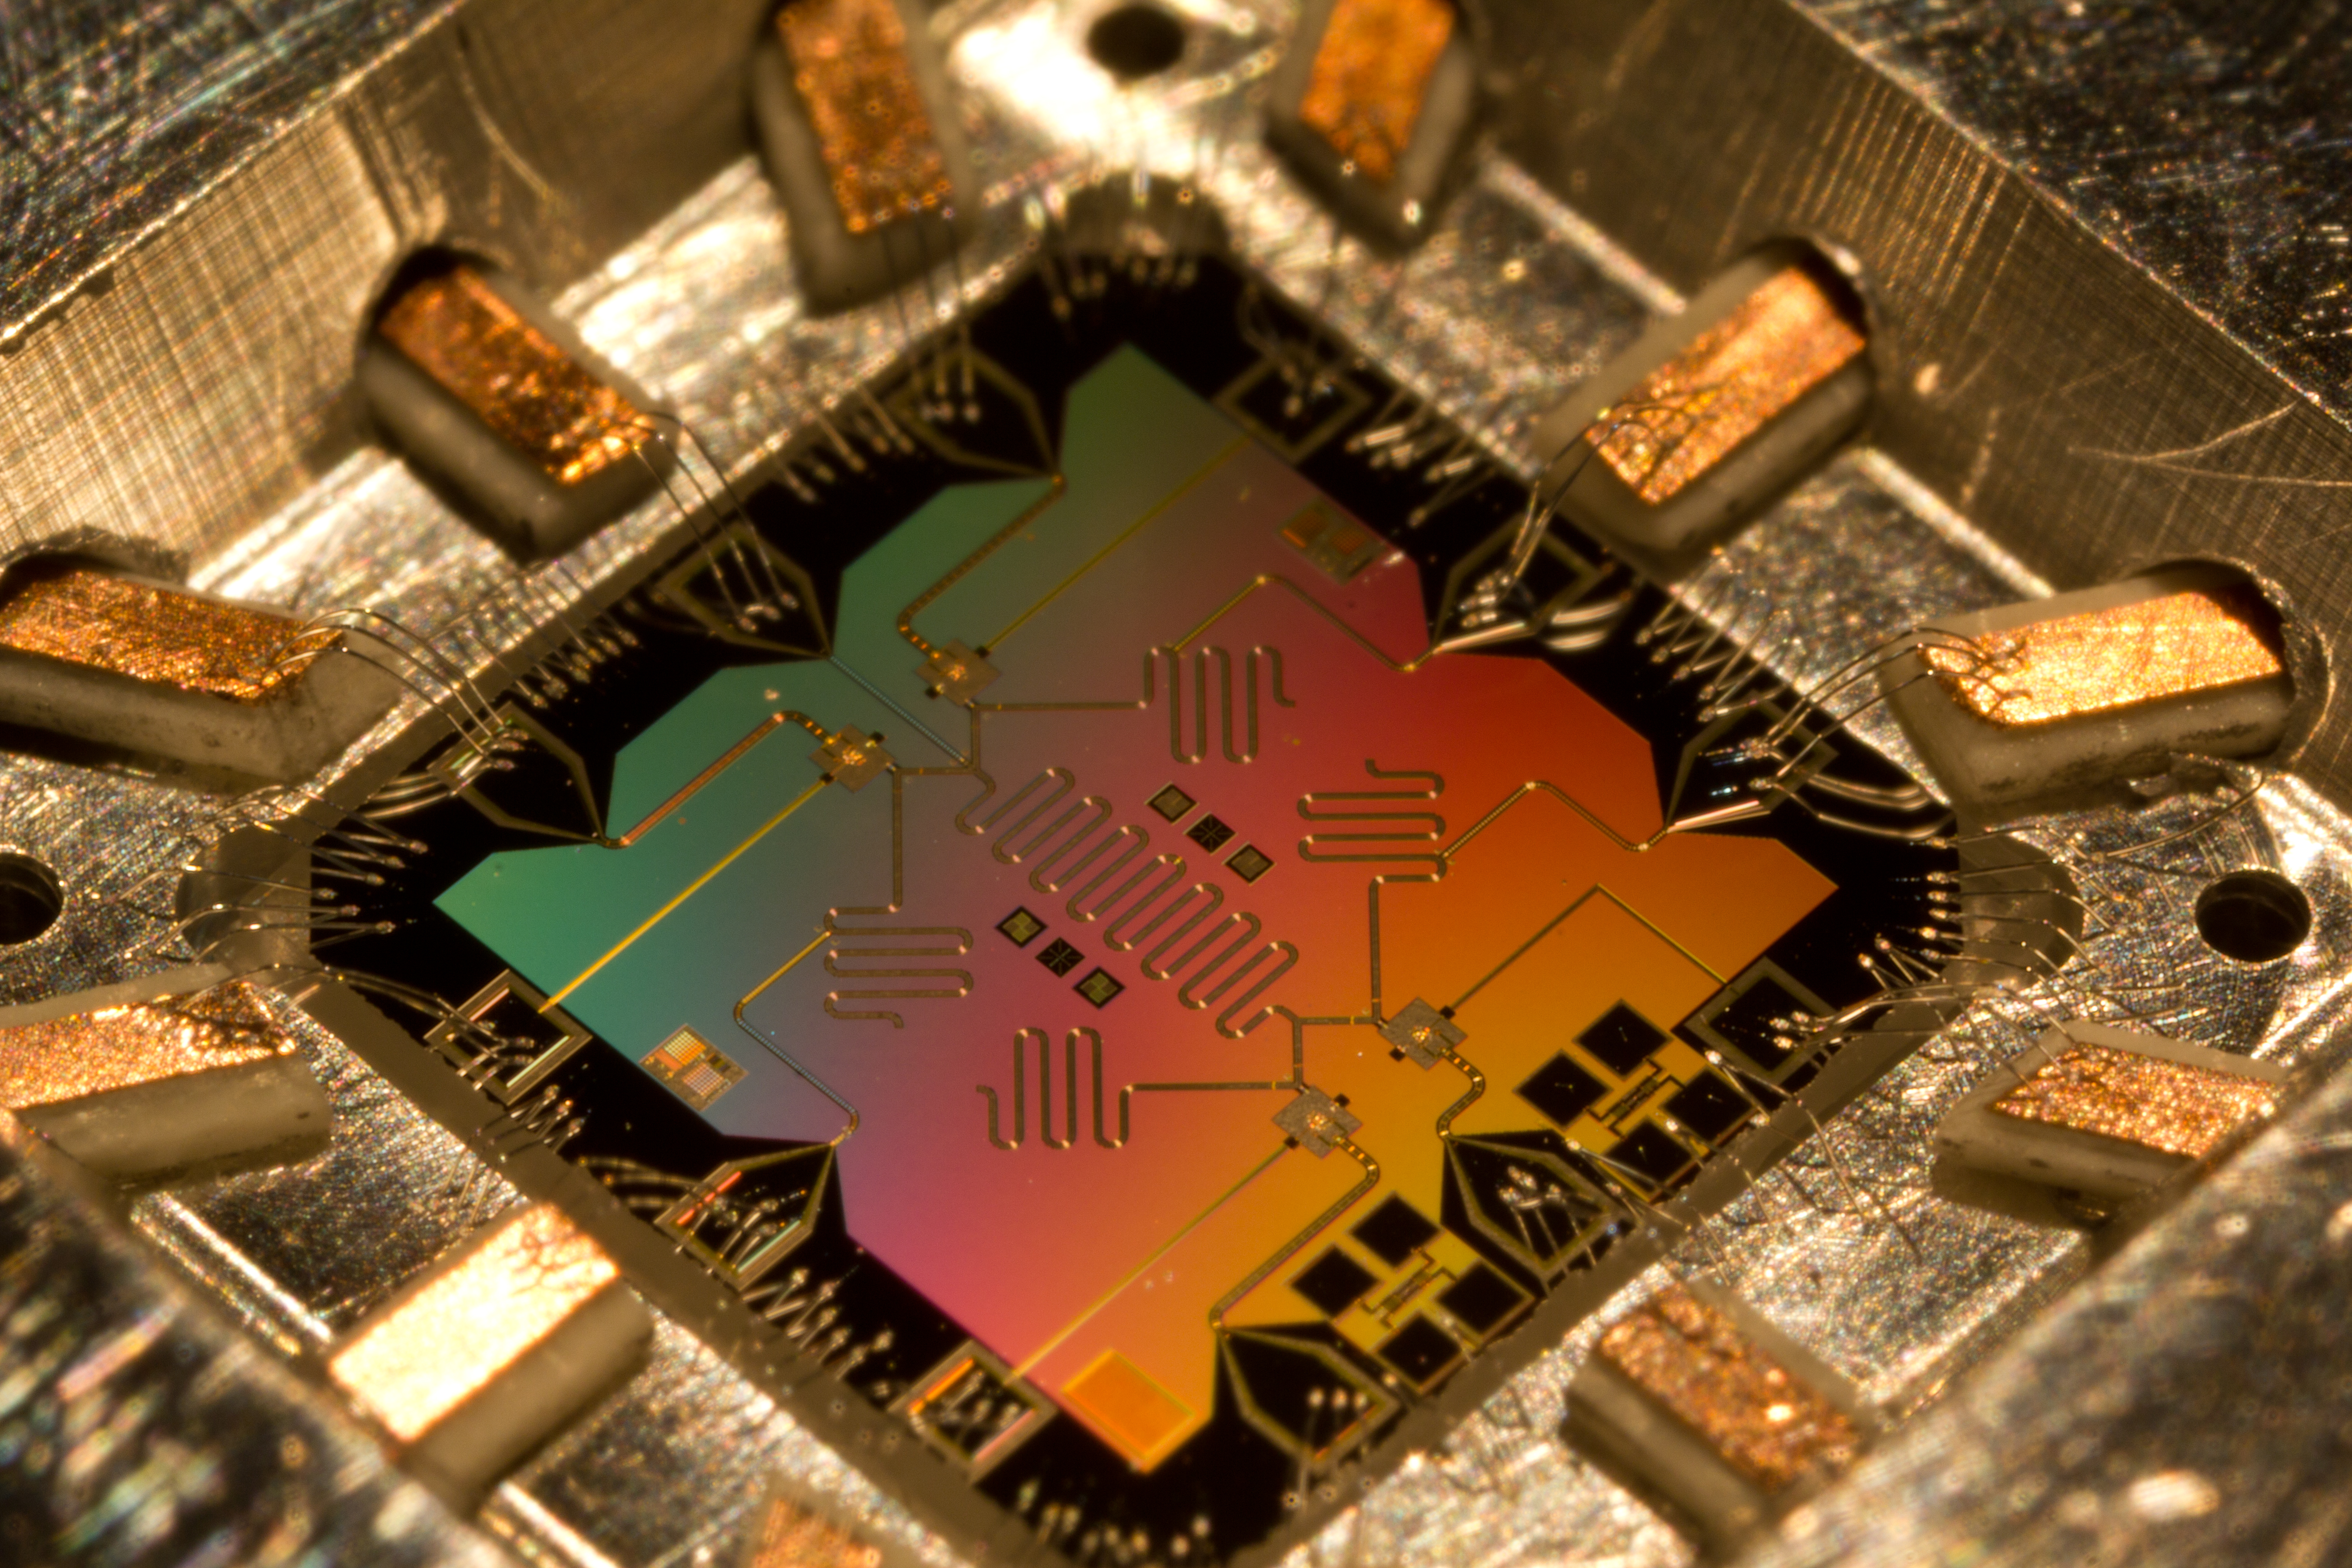
\includegraphics[width=0.6\textwidth]{figures/impl/superconductingchip.jpg}
    \caption{A superconducting chip which contains 2 qubits \cite{supercondpic} \textit{photo by Erik Lucero} \footnotemark}
    \label{fig:superconducting}
\end{figure}

\footnotetext{\url{http://web.physics.ucsb.edu/~martinisgroup/}} 
%%%%%%%%%%%%%%%%%%%%%%%%%%%%%%%%%%%%%%%%%%%%
\subsection{Linear optical quantum computing}

Linear optical quantum computing uses photons and waveguides (commonly referred to as modes) as the qubit. Using light for information processing seems like a natural choice as it is the fastest thing in the universe. Unlike trapped ions and superconducting qubits where their main problem is stopping the qubits interacting with the environment, photons interact very weakly with their environment. This is a positive as we then only have to worry about losing the photons rather than it decohering to a classical object. However, it also means that the two-qubit entangling gates are difficult to perform as photons not only interact weakly with the environment but also do not interact with each other.

Gates are currently performed using electrical heaters which heat locally a small section of the waveguide which in turn changes the phase of the photon\footnote{You can think of the phase of the photon in the same way as the phase of the electric field}. \autoref{fig:loqc} is a fully re-configurable 3 qubit integrated optical chip meaning it can perform any 3 qubit operation. The calculation is performed by using the electrically controlled phase-shifters and interference between the photons to change the probability distribution of which waveguides the photons exit the chip from. The answer to the computation is given by the which waveguides the photons exit.

\begin{figure}[H]
    \centering
    \includegraphics[width=0.7\textwidth]{figures/impl/rekkchip.png}
    \caption{Caption \cite{carolan2015universal}}
    \label{fig:loqc}
\end{figure}

%%%%%%%%%%%%%%%%%%%%%%%%%%%%%%%%%%%%%%%%%%%%
\begin{comment}
\subsection{Error Correction}

Full fault tolerance is beyond the scope of this guide however we will briefly discuss error correction. The basic idea of error correction is to use redundancy to counteract errors. Increasing the resources devoted to storing the logical information should in principle make the computer more resilient to errors.
\end{comment}

%%%%%%%%%%%%%%%%%%%%%%%%%%%%%%%%%%%%%%%%%%%%%%%%%%%%%%%%%%%%%%%%%%%%%%%%%%%%

%%%%%%%%%%%%%%%%%%%%%%%%%%%%%%%%%%%%%%%%%%%%%%%
\section{Physical gate-sets and connectivity restrictions}

Irrespective of the physical platform used to build the quantum computer we can describe the device \footnote{Assuming it is perfect and error-free} with just the gate-set and the connectivity of the device. For example the different platforms above will naturally have access to different gates. In the linear optical platform it turns out to be much easier to perform a Z gate than an X gate. Whereas we could imagine a different system where the opposite is true.

Connectivity describes which qubits are able to interact with each other\footnote{There isn't really an analogy with digital computing as the architectures are so complex we don't worry about which memory addresses are connected to each other, this is the job of the linker}. Ideally to have the most flexible and re-configurable quantum computer we would like to have full connectivity meaning all qubits are able to interact with every other. There are a number of physical implementation reasons why having many qubits connected is hard but we will not cover them here. Instead we highlight the following important fact, for a device to be universal only nearest neighbour connections are needed \autoref{fig:fullconnectivity}. Connectivity is illustrated in \autoref{fig:connectivity}. Currently, none of the devices built have achieved complete nearest-neighbour connectivity. A more likely connectivity is depicted in \autoref{fig:partialconnectivity}. This is due to imperfect fabrication of the devices.

\begin{figure}[H]
    \centering
\begin{subfigure}[h]{0.49\textwidth}
    \centering
    \includegraphics[width=\textwidth]{figures/impl/nearestneighbourcon.png}
    \caption{Full lattice type nearest-neighbour connected qubits}
    \label{fig:fullconnectivity}
\end{subfigure}
~
\begin{subfigure}[h]{0.49\textwidth}
    \centering
    \includegraphics[width=\textwidth]{figures/impl/partialnearestneighbourcon.png}
    \caption{Partially connected qubits}
    \label{fig:partialconnectivity}
\end{subfigure}
\caption{An abstraction of 8 qubit device where the lines illustrate 'connections' between qubits.}
\label{fig:connectivity}
\end{figure}

In the same way that different platforms may be suited to different gate-sets, they may also be suited to different connectivities. For example, the trapped ion platform naturally has nearest neighbour connectivity as a direct result of the tiling scheme. Compare this to LOQC or superconducting qubits where there is no intuitive design for high connectivity due to the restriction that each qubit must be connected to control electronics. Therefore, as the connectivity scales up, so does the density of control lines required, presenting serious electrical engineering challenges.

\subsubsection{Equivalence between different platforms}

Given this information we would like to be able to run a quantum program on any of the equivalent quantum devices (e.g. with the same gate-sets and connectivity). 

We can make a list of possible scenarios for different implementations of two quantum computers:
\begin{table}[h]
    \centering
    \begin{tabulary}{\textwidth}{|c|c||L|}
        \hline
        Gate-set & Connectivity & Fix  \\ \hline  
        %
        Same & Same &  Depends on what the language you have chosen to use returns, easy if both devices use the same quantum Assembly language \footnotemark  \\ \hline
        %
        Same & Different & Use a linker to remap the qubits on the devices \\ \hline
        %
        Different & Same & Use a compiler to perform gate synthesis \\ \hline
        %
        Different & Different & What classical digital compilers and linkers do \\ \hline 
    \end{tabulary}
    \caption{Required software features to convert between different quantum devices}
    \label{tab:gatesandconnectivity}
\end{table}
\footnotetext{We use Assembly here to denote the lowest level language which consists of listing instructions and which qubits the instructions act on}

%%%%%%%%%%%%%%%%%%%%%%%%%%%%%%%%%%%%%%%%%%%%%%%%%%%%

\subsection{Minimal quantum program examples}

We have chosen a minimal program which uses only classical physics, we take the binary representation of the letter 'Q' \footnote{There is nothing special about Q other than the unwritten rule of including q's when naming anything quantum related} and write the value to 8 qubits which represent a qubyte. We then measure the qubits to recover the string. Even for this simple example program we can see some differences between what goes on behind the scenes when using the built in compilers\footnote{A better description would be linker but we will get to that} and we comment on the quantum instruction set languages used. 

Like the other quantum programs above the majority of the quantum hello world program, \autoref{code:quantumhelloworldpyquil} is classical control. A small part of the algorithm uses the quantum computer. This example is novel in that there are no quantum effects used here, however it is more to illustrate the current progress of existing devices. A nice feature we have access to in the quantum case is that we can use either the bit value or phase to store information, instead of X gates an equivalent program could be written which uses H and Z gates.

\autoref{code:quantumhelloworldpyquil} shows the python input to the quantum library which passes in a bit string, the quantum simulator (or processor) is then run for each byte in the bitstring as this only requires 8 qubits. The results of each computation (measurement results) are stored in a python list and then when all of the bytes have been run on the quantum processor the bitstring is translated back into ASCII and printed using python.

We are using this example to show that quantum computers are able to do tasks that classical computers can do, a requirement if we are ever to think of building fully quantum machines (not using the co-processor model).

Even for this simple example there are a number of interesting features that all of the libraries discussed here feature:
\begin{itemize}
    \item The majority of the algorithm is classical classical control 
    \item The simulation has to be run many times to build up a an output distribution
    \item We are currently very limited by existing devices
\end{itemize}

%%%%%%%%%%%%%%%%%%%%%%%%%%%%%%%%%%%%%%%%%%%%%%%%%%%%%%%%%
\subsubsection{Translating pyQuil to quantum hardware}

To use pyQuil on a quantum processor, the source code needs to be be translated into Quil (Quantum Instruction Language) which lists the gates which must be applied to the qubits in the processor. Acts as an intermediate step between pyQuil and the actual instructions that will go to the quantum computer. The Quil compiler \footnote{\url{http://docs.rigetti.com/en/stable/compiler.html}}\footnote{We wouldn't strictly call this a compiler in the usual sense} restricts the quantum gates to the quantum devices gate-set and looks at the connectivity of the machine to make sure (2-qubit) control gates are acting on qubits that are physically connected. 

We will give an example of the compilation process in pyQuil using a simple Hello World program, shown below in \autoref{code:quantumhelloworldpyquil}. We specify the 8 qubit Agave device architecture which then maps the Quill code written to the device gate-set and connectivity. 

%%%%%%%%%%%%%%%%%%%%%%%%%%%%%%%%%%%%%%%%%%%%%%%%%%%%%%%%%%%%%%
\subsubsection{Translating QISKIT (Quantum Information Science KIT) to hardware}

The Qiskit library has to translate the python code into IBM's Open quantum assembly (OQASM) to be run on their devices. IBM has multiple quantum devices (3, 4, 5 and 16 qubit devices) that you can run quantum programs on. Qiskit also comes with a local simulator, similar to pyQuil which can simulate up to 32 qubits. An API key is needed to access the quantum devices but not the local simulator.

Here we give an example of the Qiskit python library code and the OQASM output \footnote{the user can write QASM embedded in Python and Qiskit will return the program as QASM \footnotemark} \footnotetext{There is no spelling mistake here...}. We tried compiling the OQASM to a device specific arcitecture but couldn't get the program to reduce or simplify the gates.

%%%%%%%%%%%%%%%%%%%%%%%%%%%%%%%%%%%%%%%%%%%%%%%%%%%%%%%%%
\subsubsection{Translating Project Q to hardware}

ProjectQ is one of the more flexible quantum programming languages available in terms of the types of operations, compilers and back-ends that are available. Many of the typical gates that are used in quantum algorithms are already built in, and user defined gates that are either just matrices or based on mathematical operations are relatively simple to implement. 

Project Q is also the only library discussed here that comes with a local simulator. You can also a specify machine architecture for IBM devices using the IBM compatible compiler \cite{zulehner2018efficient} which will compile the project Q code into the gate-set and connectivity of the specified machine.
%%%%%%%%%%%%%%%%%%%%%%%%%%%%%%%%%%%%%%%%%%%%%%%%%%%%%%%%%
\subsubsection{Translating Q\# to hardware}

It is not currently possible to convert code written in Q\# to hardware. This is because there is only a simulator and no way to obtain the list of gates that are being simulated. We have therefore not included a minimal example of compiling Q\# code to hardware level instructions.

Q\# does however support a resource counter which estimates the resources required to run the quantum program on hardware. We give a minimimal example showing 

%%%%%%%%%%%%%%%%%%%%%%%%%%%%%%%%%%%%%%%%%%%%%%%%%%%%%%%%%
% code
\noindent \begin{minipage}[t]{0.45\textwidth}
\begin{listing}[H]
   \inputminted{python}{code/asm/pyquil_helloworld.txt} 
    \caption{Pyquil Hello Q program}
\end{listing}
\end{minipage} \hfill 
\begin{minipage}[t]{0.45\textwidth}
\begin{listing}[H]
   \inputminted[lastline=15]{python}{code/asm/pyquil_helloworld_output.txt}
   \caption{Quil code from pyQuil code}
\end{listing}
\begin{listing}[H]
   \inputminted[firstline=17, lastline=37]{python}{code/asm/pyquil_helloworld_output.txt}
   \caption{Compiled code using the 8 qubit AGAVE devce architecture}
\end{listing}
\end{minipage}

%%%%%%%%%%%%%%%%%%%%%%%%%%%%%%%%%%%%%%%%%%%%%%%%%%%%%%%%%%%%%%

%%%%%%%%%%%%%%%%%%%%%%%%%%%%%%%%%%%%%%%%%%%%%%%%%%%%%%%%%%%%%%
% code
\noindent \begin{minipage}[t]{0.55\textwidth}
\begin{listing}[H]
   \inputminted{python}{code/asm/text/progqiskithello.txt}
   \caption{Qiskit hello world}
\end{listing}
\end{minipage} \hfill 
\begin{minipage}[t]{0.3\textwidth}
\begin{listing}[H]
   \inputminted[firstline=2,lastline=18]{python}{code/asm/qiskit_helloworld.output.txt}
   \caption{OQASM for the qiskit hello world program}
\end{listing}
\begin{listing}[H]
   \inputminted[firstline=21]{python}{code/asm/qiskit_helloworld.output.txt}
   \caption{OQASM for the qiskit hello world program}
\end{listing}
\end{minipage}


\begin{comment}
\url{https://github.com/Qiskit/qiskit-terra}
\url{https://github.com/Qiskit/openqasm/tree/master/examples}
\url{https://github.com/Qiskit/qiskit-tutorial/blob/master/reference/algorithms/grover_algorithm.ipynb}
\url{https://github.com/Qiskit/qiskit-tutorial/blob/master/appendix/advanced_qiskit/compiling_and_running.ipynb}
the qiskit backends are here \url{https://github.com/Qiskit/qiskit-backend-information/tree/master/backends}
QASM documentation here \url{https://github.com/Qiskit/openqasm/blob/master/spec/qasm2.rst}
The Qiskit compiler \url{https://developer.ibm.com/code/2017/05/17/developers-guide-to-quantum-qiskit-sdk/}
\end{comment}
%%%%%%%%%%%%%%%%%%%%%%%%%%%%%%%%%%%%%%%%%%%%%%%%%%%%%%%%%%%%%%

%%%%%%%%%%%%%%%%%%%%%%%%%%%%%%%%%%%%%%%%%%%%%%%%%%%%%%%%%%%%%%
% code
\noindent \begin{minipage}[t]{0.6\textwidth}
\inputminted{python}{code/asm/text/progprojqhello.txt}
\end{minipage} \hfill 
\begin{minipage}[t]{0.37\textwidth}
\inputminted[lastline=29]{python}{code/asm/projqout.txt}
\inputminted[firstline=31]{python}{code/asm/projqout.txt}
\end{minipage}

\subsubsection{Q\# example}

That's right. There is no example.

%%%%%%%%%%%%%%%%%%%%%%%%%%%%%%%%%%%%%%%%%%%%%%%%%%%%%%%%%%%%%%
\subsection{Summary}

We now compare some of the implementation dependent features of the languages and give a comparison between them.
%%%%%%%%%%%%%%%%%%%%%%%%%%%%%%%%%%%%%%%%%%%%%%%%%%%%%%%%5
\subsubsection{Qubit management}

The pyQuil qubit management is dynamic, qubits are allocated dynamically which does not require the users input. The qiskit library is heavily based on using quantum circuits. You specify quantum and classical registers and ancilla qubits. Project Q also requires the user to manually allocate qubits and the QASM resembles dynamically allocated qubits with allocate and deallocate at the start and end of the instruction set. 

%%%%%%%%%%%%%%%%%%%%%%%%%%%%%%%%%%%%%%%%%%%%%%%%%%%%%%%%5
\subsubsection{Compilers/Gate simplification}

All of the libraries have access to the standard gate set in their python environments\footnote{X,Y,Z,H,Phase gates and arbitrary rotations}. 

In pyQuil the user can also use the \texttt{defgate()} method to define their own gate either in terms of compositions of existing gates or by specifying a matrix representation of the gate. Qiskit also can define gates. Project Q has the option to define gates?

The pyQuil compiler takes one of Rigetti's quantum devices as an argument and compiles their Quill QASM into device specific gate-set and remaps the qubits to match the connectivity of the machine.

IBM has no working compiler\footnote{there is a compiler but it does nothing, specify x only and the program crashes, specify x and H and the program uses Z. U(x,y,z)($\theta$).} but we can return the Open QASM (IBM's Quantum Assembly format), 

The Project Q compiler is designed to have a modular structure, so the user can pick and choose the level of optimisation required. It works quite well although you have to manually specify the available gate-set you have access to and the connectivity of the machine. They are working on adding in backend support for the IBM quantum devices.


%%%%%%%%%%%%%%%%%%%%%%%%%%%%%%%%%%%%%%%%%%%%%%%%%%%%%%%%5
\begin{comment}
\subsubsection{Resource counters}

All of the software packages support resource counting of some sort.

\end{comment}
%%%%%%%%%%%%%%%%%%%%%%%%%%%%%%%%%%%%%%%%%%%%%%%%%%%%%%%%5
\subsubsection{Backends}

Rigetti then offers a remote Quantum Virtual Machine (QVM) which runs simulations of up to 26 qubits requiring an API key to use. They do not provide a local simulator which runs on a personal computer. IBM do provide a local simulator and access to their devices and remote simulator require and API key. Project Q comes with a local simulator, written in c++ and is built on your machine on install using python wrappers.

The project Q simulator is best of the local simulators however currently there is no way to compile project Q code into IBM's OASM to run on IBM's machines or compile to Quil to run on Rigetti's machines. Although IBM and Project Q existed as part of the same project \footnote{see git change-log} we are unsure of when the project Q to IBM backend will be implemented. 

One slightly annoying feature of pyQuil the software package is the lack of local quantum simulator. This can cause problems when trying to execute large programs as we often found the connection timed out before the program finished. 

%%%%%%%%%%%%%%%%%%%%%%%%%%%%%%%%%%%%%%%%%%%%%%%%%%%%%%%%5
\subsubsection{Device mappings}

Rigetti's Quil compiler takes a dictionary of one of their devices which then creates a map of the positions of the qubits and the connectivity of the machine. 

QISKits' \texttt{get remote backends} method doesn't return any valid devices to compile to, when using one of their device names an error saying the device is not valid is produced. It may be possible to manually add device mappings but even then the \textit{compiler} didn't compile to the given gate-set or it would produce an error for some gate-sets.

Project Q lets you specify the connectivity using a Python dictionary and gate-set by importing the gates you want/have access to. The compiler works quite well.

\section{Comparing classical and quantum compilers}

In the previous section we showed how quantum compilers work. They take source code (for example pyQuil) and turn it into a low level set of operations (for example Quil) which can be executed on a quantum device or simulator. The compiler performs certain optimisation operations (for example simplifying $HZH$ to $X$) but does not otherwise substantially modify the source code. 

Here we show, by way of comparison, the compilation steps that turn a classical program (Hello world, written in C) into an executable file. Our aim is to show that there are many more steps in the process, including optimisation and linking, which are not really present in the quantum case. We will discuss in detail what each of these steps are, why they are necessary and how they occur in a classical computer. We will then speculate on which of how quantum compilation may eventually develop as the complexity of quantum programs increases.

\begin{comment}

Quantum compilers have a range of meaning depending on who you ask, we hope to clarify some of the common misconceptions\footnote{The use of compiler is abused in all of the quantum libraries discussed here} in the following section. 


We give an example of a simple Assembly program. Much like the the \textit{quantum languages} covered in this guide, assembly code is contains a list of operations, drawn from an instruction set, that the computer should perform. 


Unlike interpreted languages, assembly needs to first be assembled and then linked. Assembling is the process which turns assembly language into object code -- this is a small block of machine code which cannot be directly executed because none of its contents (variables etc.) have memory addresses yet. The linker takes an object file and produces an executable file where all the addresses are properly defined. The linker can also process multiple object files, producing a single executable file. The linker provides flexibility in allocating the resources needed to run a program. Below we give some examples illustrating the purposes of compilers and linking.

We now include a \textit{Hello world!} program, even in this simple program case we can see that the linker is important.
\end{comment}



%%%%%%%%%%%%%%%%%%%%%%%%%%%%%%%%%%%%%%%%%%%%%%%%%%%%%%%%%
\subsection{Compile, Assemble, link, execute}

As shown in \autoref{fig:compileasslinkrun}, there are three steps which turn a classical compiled language such as C into a program which can be executed on a classical computer. We will demonstrate this process in the case of a simple \textit{Hello World!} program written in C. The program prints the string "Hello World!" and exits, returning 0 to the operating system. This is shown in \autoref{code:c_helloworld}.

\noindent \begin{minipage}{0.65\textwidth}
% c code
\begin{listing}[H]
   \inputminted{c}{code/asm/c_helloworld.txt}
   \caption{Hello world! in C}
   \label{code:c_helloworld}
\end{listing}

The compiler takes this C source file as an input, and outputs the assembly language file shown in \autoref{code:asm_helloworld}. The assembly file looks very different to the original source code, because it contains instructions like movl and call. These instructions performs a basic operations such as moving data around or calling sub-routines. There is normally a large degree of optimisation that goes into this step, because the language constructs in C do not map directly to instructions in assembly language. 

% asm code
\begin{listing}[H]
   \inputminted[firstline=8, lastline=22]{gas}{code/asm/c_helloworld.x86_64.txt}
   \caption{Assembly file after compiling}
   \label{code:asm_helloworld}
\end{listing}
\end{minipage} \hfill
%
\begin{minipage}{0.3\textwidth}
    \centering
    \includegraphics[width=1.1\textwidth]{figures/impl/compileassemblelinkrun.png}
    \captionof{figure}{Compile, assemble, linking and running structure for running a program}
    \label{fig:compileasslinkrun}
\end{minipage}

The assembler then turns the assembly language file into an object file, shown in the left hand part of \autoref{code:obj_helloworld}. This is quite a simple step -- it involves replacing all the instructions with strings of numbers called machine code which is readable by the target computer. The right hand column shows the instructions corresponding to the codes on the left. The critical feature of the object file is the lack of addresses. For example lines 3 and 4 contain placeholders \$0x0 and e. These addresses are resolved by the linker, which assigns memory to all the variables. The linked file is shown in \autoref{code:exe_helloworld}. Notice how the program itself has also been assigned a memory location -- line 1 shows that the first instruction is at address 400526. In larger programs, each source file has its own object file. The linker combines all these files together to produce an executable file which can be run on the target computer.

% object filoe
\begin{listing}[H]
   \inputminted[firstline=40, lastline=46]{gas}{code/asm/c_helloworld.x86_64obj.txt}
   \caption{Object file before linking}
   \label{code:obj_helloworld}
\end{listing}

\begin{listing}
   \inputminted[firstline=137, lastline=143]{gas}{code/asm/c_helloworld.x86_64obj.txt}
   \caption{Executable file after linking}
   \label{code:exe_helloworld}
\end{listing}

%%%%%%%%%%%%%%%%%%%%%%%%%%%%%%%%%%%%%%%%%% tikz
\begin{comment}
\tikzstyle{every picture}+=[remember %picture,inner xsep=0,inner ysep=0.25ex]

% c prog
\begin{code}
\inputminted[]{c}{code/asm/c_helloworld.txt}
\captionof{listing}{Hello world! in C 
\tikz[remember picture] \node [] (a){ };}
\label{code:c_helloworld}
\end{code}


\begin{tikzpicture}[remember picture, overlay]
\draw[->, line width=1mm] (a.south) -- %++(0,-2ex) node[anchor=north] {Compiler} -| %(b.north) ;  
\end{tikzpicture}

%% compiled c prog
\begin{code}
\tikz[remember picture] \node [] (b) {};
\inputminted[firstline=8,lastline=22]{gas}{code/asm/c_helloworld.x86_64.txt}
\captionof{listing}{Assembly code of Hello world! in C 
\tikz[remember picture] \node [] (c) {};}
\end{code}

\begin{tikzpicture}[remember picture, overlay] 
\draw[->, line width=1mm] (c.south) -- %++(0,-1.5ex) -| (d.north) ;
\end{tikzpicture}

%% assembled c prog
\begin{code} 
\tikz[remember picture] \node [] (d) {};
\inputminted[firstline=37,lastline=46]{objdump}{code/asm/c_helloworld.x86_64obj.txt}
\captionof{listing}{Object dump of the Hello world assembled object file 
\tikz[remember picture] \node [] (e) {};}
\end{code}

\begin{tikzpicture}[remember picture, overlay]
\draw[->, line width=1mm] (e.south) -- ++(0,-1.5ex) -| (f.north) ;
\end{tikzpicture}

% linked c prog
\begin{code} 
\tikz[remember picture] \node [] (f) {};
\inputminted[firstline=60,lastline=74]{objdump}{code/asm/c_helloworld.x86_64obj.txt}
\captionof{listing}{Object dump of the executable program after compiling, assembling and linking, we have truncated the code early here.
\tikz[remember picture] \node [] (g) {};}
\end{code}


%%%%%%%%%%%%%%%%%%%%%%%%%%%%%%%%%%%%%%%%%%%%%%%%
\begin{tikzpicture}[overlay]
    % Bend above text line
    %\draw[-latex] (node2.north) to[bend right] (node1.north);
    % Bend below text line
    %\draw[-latex] (node2.south) to[bend left] (node1.south);
    % Angled
    \draw[-latex] (node5.south) -- ++(0,-1.5ex) -| (node6.north);
\end{tikzpicture}
\end{comment}
%%%%%%%%%%%%%%%%%%%%%%%%%%%%%%%%%%%%%%%%%%%%%%%%%

%%%%%%%%%%%%%%%%%%%%%%%%%%%%%%%%%%%%%%%%%%%%%%%%%%%%%%%%%%%%%%%%%%%%
\subsection{Quantum compilation}

\begin{wrapfigure}{r}{0.4\textwidth}
    \centering
    \includegraphics[width=0.45\textwidth]{figures/impl/quantumcompilefixrun.png}
    \caption{quantum instruction set flow}
    \label{fig:quantumcompile}
    \vspace{-30pt}
\end{wrapfigure}

Quil, OQASM and Project Q's quantum assembly have laid the ground work for building a quantum programming language. Although we suspect it will be some time before we get a full quantum language and not domain specific embedded languages, the work on quantum instruction sets has a long way to go. 

The main feature we would like to highlight is that because Assembly is such a low-level language, the program is doesn't need to be compiled, the action of the assembler and linker is to rename the human readable code into machine code and allocate memory for the program. This is exactly the same as the quantum libraries discussed here \footnote{see the cloud based section, the python code and \textit{compiled} code are relabelings of each other}.

quantum computers have linkers at the moment. what a compiler is and should be for quantum computer. The assembler process which assigns temporary addresses to parts of the object file is similar to a lot of the resource counting steps that the current quantum libraries and languages have.

%%%%%%%%%%%%%%%%%%%%%%%%%%%%%%%%%%%%%%%%%%%%%%%%%%%%%%%%%%%%%%%%%%%%%%%%

%\begin{verbatim}
%% TODO IN A LATER VERSION. :(

%%%%%%%%%%%%%%%%%%%%%%%%%%%%%%%%%%%%%%%%%%%%%%%%%%%%%%%%%%%%%%%%%%%%%%%%
%                                                                      %
%%%%%%%%%%%%%%%%% RIP FORTRAN YOU MAGNIFICENT BASTARD %%%%%%%%%%%%%%%%%%
%                                                                      %
%%%%%%%%%%%%%%%%%%%%%%%%%%%%%%%%%%%%%%%%%%%%%%%%%%%%%%%%%%%%%%%%%%%%%%%%

%%%%%%  %%%%%%%%    %%%%%%   %%%%%%%    %%%%%%         %       %       %
%       %      %    %     %     %       %     %       % %      % %     %
%%%%%   %      %    %   %       %       %   %        % % %     %   %   %
%       %      %    %    %      %       %    %      %     %    %    %  %
%       %%%%%%%%    %     %     %       %     %    %       %   %     % %

% this took longer than you'd think
%\end{verbatim}


%
%%%%%%%%%%%%%%%%%%%%%%%%%%%%%%%%% END OF USEFUL CONTENT
%

\begin{comment}

\subsubsection{Rigetti's Forest}

We will now discuss in detail the structure of what happens when the code examples above are run. For Rigetti \url{http://docs.rigetti.com/en/stable/compiler.html#region-specific-compiler-features-through-pragma}

The structure of Rigetti's quantum programming environment is as follows:
\begin{itemize}
    \item \textbf{Forest} - Rigetti's entire quantum programming toolkit. Overall the Forest documentation is very good\footnote{\url{docs.rigetti.com/en/stable/}}
    \item \textbf{pyQuil} - Open source Python library. The user writes their code in pyQuil\footnote{There is a kind of standard library for pyQuil called Grove} and this gets translated to Quil .
    \item \textbf{Quil} – Quantum Instruction Language which is assembly-like as it lists the gates to apply. Acts as an intermediate step between pyQuil and the actual instructions that will go to the quantum computer.
    \item \textbf{Execution} Rigetti has a Quantum Virtual Machine \textbf{QVM} which runs simulations of up to 26 qubits - an API key is required to access this. (They do not provide a local simulator.) They also have Quantum Processing Units \textbf{QPUs}, which are actual chips with physical qubits which requires special access.
\end{itemize}

%%%%%%%%%%%%%%%%%%%%%%%%%%%%%%%%%%%%%%%%%%%%%%%%%%%%%
\subsubsection{IBM's QISKIT (Quantum Information Science KIT)}


The current state of IBM's stack, from top to bottom consists of the following elements:

\begin{itemize}
    \item \textbf{QISKit} - IBM's open source quantum library for usage in the high level language Python \footnote{There is a standard library for algorithms called ACQUA}.
    \item \textbf{OpenQASM} – IBM's low-level Quantum Assembly Language which interprets commands and functions from QISKit and translates them into microwave pulses for use on the physical architecture (superconducting qubits). Acts as an intermediate step between QISKit and the actual instructions that will go to the quantum computer.
    \item \textbf{Execution} \textbf{QPU} - IBM has multiple physical architectures for running quantum algorithms. These include 3, 4, 5 and 16 qubit devices accessible via an API provided when you create an account with the IBM Experience, and larger 20 qubit devices that are available via membership to the IMB Q Network (hubs, partner institutions etc). \textbf{Q QASM Simulator} - IBM's Quantum Virtual Machine which runs simulations of up to 32 qubits, an API key is required to access this.
\end{itemize}

The devices used to perform the simulation and computation are based on a superconducting charge qubit implementation, which can be found described in more detail in \autoref{chpt:implementations}. 

Open QASM is their quantum assmbely language, Qiskit is the Quantum Information Science Kit which is a python library where the user can write QASM and Qiskit will translate it into QASM \footnote{somehow but I haven't figured it out yet...}. 


%%%%%%%%%%%%%%%%%%%%%%%%%%%%%%%%%%%%%%%%%%%%%%%%%%%%%%%%%
\subsubsection{Project Q}

\begin{figure}[h]
    \centering
    \includegraphics[width=\textwidth]{projectq_structure.PNG}
    \caption{Structure of ProjectQ. Taken from \cite{projectq2018}, will make own diagram and possibly simplify.}
\end{figure}

ProjectQ is one of the more flexible quantum programming languages available in terms of the types of operations, compilers and back-ends that are available. Many of the typical gates that are used in quantum algorithms are already built in, and user defined gates that are either just matrices or based on mathematical operations are relatively simple to implement. 

\begin{itemize}
    \item Python library
    \item Local simulator
    \item Can specify machine architecture for IBM devices
\end{itemize}
%%%%%%%%%%%%%%%%%%%%%%%%%%%%%%%%%%%%%%%%%%%%%%%%%%%%%%%%%

%%%%%%%%%%%%%%%%%%%%%%%%%%%%%%%%%%%%%%%%%%%%%%%%%%%%%%


\end{comment}


\begin{comment}
% code
% left side
\begin{minipage}[t]{0.4\textwidth}
\begin{code}
\captionof{listing}{Hello world! in C}
\inputminted[]{c}{code/asm/c_helloworld.txt} 
\end{code}
\end{minipage} \hfill 
% right side
\begin{minipage}[t]{0.6\textwidth}
\begin{code}
\captionof{listing}{Assembly code of Hello world! in C}
\inputminted[]{gas}{code/asm/c_helloworld.x86_64.txt}
\end{code}
\end{minipage}

The compiler has completely changed the C function into Assembly code. 

The next step is to assemble the assembly code into an object file,

% code
%{\renewcommand\fcolorbox[4][]{\textcolor{cyan}{\strut#4}}
% left side
%\begin{minipage}[t]{0.49\textwidth}
\begin{code}
\inputminted[firstline=32, lastline=51]{objdump}{code/asm/c_helloworld.x86_64obj.txt} 
\captionof{listing}{Object dump of the Hello world assembly file}
\end{code}
%\end{minipage} \hfill 
% right side
%\begin{minipage}[t]{0.49\textwidth}

after assembling the file we now have to link the file to assign actual memory locations.
\begin{code}
\inputminted[firstline=55, lastline=74]{objdump}{code/asm/c_helloworld.x86_64obj.txt}
\captionof{listing}{Object dump of the executable program after compiling, assembling and linking, we have truncated the code early here.}
\end{code}
\end{comment}
%\end{minipage}
%}


%FORTRAN and C are both functional languages and follow a clear structure

\begin{comment}
\subsubsection{x86 Assembly}
% program
%\lstinputlisting[language=Asmx86, firstline=1, lastline=25, caption={Hello world program}, label={code:helloworldasm}]{code/asm/printobj.txt}

\begin{code}
\inputminted[firstline=2, lastline=25]{gas}{code/asm/printobj.txt}
\captionof{listing}{Hellow world program in x86 asm}
\label={code:helloworldasm}
\end{code}
The program when run returns the string \textit{Hello World} to the terminal. In order to run the program we must assemble and then link the object file. Assembling the program produces an object file, we can dump the contents of the file and look at what the assembler does to a program,

% assembled
%\lstinputlisting[language=Asmx86, firstline=27 , lastline=48, caption={Hello world assembled}, label={code:assembledhelloworldasm}]{code/asm/printobj.txt}
\begin{code}
\inputminted[firstline=28,lastline=48]{objdump}{code/asm/printobj.txt}
\captionof{listing}{Hello world assembled}
\label={code:assembledhelloworldasm}
\end{code}

\autoref{code:assembledhelloworldasm} is the assembled object dump for the \textit{Hello world} program. The assembler has given temporary memory addresses to the object file. This is similar to a lot of the resource counting steps that the current quantum libraries and languages have. 

In order to produce executable code we have to link the object which assigns it actual memory locations. Linking can be done using the GNU Linker, \textit{ld}. This produces another file which we can view using objectdump to see what the linker has done.

% linked
%\lstinputlisting[language=Asmx86, firstline=51 , lastline=72, caption={Hello world assembled and linked}, label={code:linkedhelloworldasm}]{code/asm/printobj.txt}

\begin{code}
\inputminted[firstline=52, lastline=72]{objdump}{code/asm/printobj.txt}
\captionof{listing}{Hello world assembled and linked}
\label{code:linkedhelloworldasm}
\end{code}

\autoref{code:linkedhelloworldasm} is the linked and assembled code for the \textit{Hello world} program Now the memory locations have been assigned to the code.

\autoref{code:assembledhelloworldasm} is the dump of the assembled object code and \autoref{code:linkedhelloworldasm} is the dump of the assembled and linked object code. 
\end{comment}


%%%%%%%%%%%%%%%%%%%%%%%%%%%%%%%%%%%%%%%%%%%%%%%%%%%%%%%%%%%%%%%%%%%%%%%%

%\begin{verbatim}
%% TODO IN A LATER VERSION. :(

%%%%%%%%%%%%%%%%%%%%%%%%%%%%%%%%%%%%%%%%%%%%%%%%%%%%%%%%%%%%%%%%%%%%%%%%
%                                                                      %
%%%%%%%%%%%%%%%%% RIP FORTRAN YOU MAGNIFICENT BASTARD %%%%%%%%%%%%%%%%%%
%                                                                      %
%%%%%%%%%%%%%%%%%%%%%%%%%%%%%%%%%%%%%%%%%%%%%%%%%%%%%%%%%%%%%%%%%%%%%%%%

%%%%%%  %%%%%%%%    %%%%%%   %%%%%%%    %%%%%%         %       %       %
%       %      %    %     %     %       %     %       % %      % %     %
%%%%%   %      %    %   %       %       %   %        % % %     %   %   %
%       %      %    %    %      %       %    %      %     %    %    %  %
%       %%%%%%%%    %     %     %       %     %    %       %   %     % %

% this took longer than you'd think
%\end{verbatim}


%
%%%%%%%%%%%%%%%%%%%%%%%%%%%%%%%%% END OF USEFUL CONTENT
%

%%%%%%%%%%%%%%%%%%%%%%%%%%%%%%%%%%%%%%%%%
%%%%%%%%%%%%%%%%%%%%%%%%%%%%%%%%%%%%%%%%%%%%%%%%%%%
\section{Quantum software architecture}
% classical structure
Computer languages are influenced by the structure of the computer. In classical computers, languages developed historically in order to increase abstraction and ease the task of the programmer. To begin with, assembly language replaced machine code because it is easier to remember a mnemonic like ADD rather than a string of ones and zeros representing the same thing. The C programming language was invented to make common programming constructions such as if-statements and while-loops easier to program, using machine independent syntax. C is a compiled language, meaning that it needs to be converted into machine code before it can run. There is a different compiler for each computer architecture, which converts C into the specific instructions that can be executed on that machine. 

\begin{figure}[H]
    \centering
    \includegraphics[width=\textwidth]{figures/impl/cpuqpu.png}
    \caption{Caption}
    \label{fig:my_label}
\end{figure}

%abstraction oop or functional
Other levels of abstraction have subsequently been introduced into programming. Some relate to code structure (object oriented programming, functional programming, and other paradigms), and others to the portability of the code. For example, Java runs in an environment called a virtual machine. This is a program which runs a file containing Java source code on a particular computer. The critical difference between this and a compiler is that many computers have a Java virtual machine, so that the end user can just run the same program without having to worry about whether there is a compiler present. 

% nisq devices birth of languages
Quantum programming languages may eventually develop in a similar way. However, there are some important differences. For example, quantum programming languages are being developed without there existing a large scale quantum computer to run programs on. This is due to the hindsight afforded by classical programming languages, and the assumption that quantum programming languages will be essentially similar. Their role is currently to understand the structure of quantum algorithms better and to provide a platform for simulating quantum computers, rather than to make programming quantum computers easier. 

% bad to do single qubits quantum computer with structure
Here, we will consider how the implementation of a large scale quantum computer might inform the structure of quantum languages. For example, most quantum programming languages currently emphasise single qubit manipulation. While this works when we only have a few qubits, it clearly becomes unfeasible in a quantum computer with a million qubits. There, it will be necessary to organise qubits into registers, variables and types depending on their role. What should those types be? How should it be informed by the structure of the quantum computer?

% re configurable logic and memory sections
Part of the issue is the current lack of understanding of large scale quantum computer architectures. A typical classical computer CPU architecture is shown in \autoref{fig:cpuHarvArch}. It contains modules for memory, processing and arithmetic, buses for moving data around, and input/output ports to connect to other devices. The computer is controlled by an instruction set, which is read and decoded in the control section. 

Each instruction performs a basic operation such as moving data from external memory into working memory, adding variables together, etc. There are also control instructions for deciding what to do next, for example branches and sub-routine calls. Memory is often organised into registers, which might be 8 bits wide in a small microcontroller, or 64 bits wide in a modern Intel processor. These instructions are the lowest level of processing available to a classical programming language. 
% 
By analogy, it is likely that a quantum computer will have a similar architecture containing an instruction set (ADD, MOV, etc.). We will consider the possible structure of such an instruction set in \autoref{sec:qinstructions}. We will then consider the simplest type of abstraction above quantum assembly language -- the analogue of C (QLang+-!). We will consider the necessity of quantum compilers and linkers, and how they differ from their classical counterparts in (section). 

%%%%%%%%%%%%%%%%%%%%%%%%%%%%%%%%%%%%%%%%%%%%%%%%%
\subsection{Quantum instruction sets}
\label{sec:qinstructions}

An instruction set is a collection of operations designed to meet two competing requirements. The instructions must contain enough operations to allow access to the full functionality of the computer, without exposing implementation details. Further, it must be simple to express a program in terms of the instruction set, so the instructions should be as high level as possible. However, the instruction set should not be overly large or contain complex operations, otherwise it would be difficult to implement in hardware.

Candidate instruction sets could therefore tend towards two opposite extremes. On the one hand, the instruction set could be very large and implement nearly everything a program might want to do: matrix multiplication, Fourier transforms, database operations, etc. Every operation would be optimised in hardware and all possible tasks would be accounted for. This would make programming and compiling very simple and programs would tend to be very efficient. However, the instruction set would be difficult to implement, and inflexible in the face of new applications and tasks.

On the other end of the scale, the instruction set might be the single operation NAND. This would be universal for classical computation, so all programs could be realised. The design of the computer would be very simple, with only one instruction to implement. However, simple programming tasks such as addition would become very difficult, and complicated programs would be nearly impossible to write.

Classical instructions sets sit between these two extremes. They contain general operations such as arithmetic (ADD, MUL, etc.), copy operations (MOV) and control flow (BRANCH, CALL, etc.) and they also contain some lower level details such as bit manipulation. 

In the rest of this section we consider the instructions which might form the basis of a full quantum computer.

%%%%%%%%%%%%%%%%%%%%%%%%%%%%%%%%%%%%%%%%%%%%%%%%%%%%%%

\subsubsection{Qubit manipulation}

Despite the need for full quantum computers to contain operations on registers, it is likely that they would retain single qubit manipulation. In classical computers single bits can be accessed using bit manipulation instructions.  For example, in the Microchip 16-bit dsPIC family of microcontrollers \cite{microchip2008AsmRef}, bits can be set to zero or one using the BCLR and BSET instructions.

\begin{lstlisting}[language=asm, caption={Single bit operations}]
    CLR     w0      ; clear register w0
    CLR     w1      ; clear register w1
    BSET    w0, #2  ; set bit #2 of register w0 to 1
    BTG     w1, #6  ; toggle bit #6 of register w1
    BCLR    w1, #5  ; clear bit #5 of register w1
\end{lstlisting}

This code initialises the two registers w0, w1 to zeroes, puts a one in the second bit of register w0, and a zero in the fifth bit of register w1. The BTG instruction toggles bit six of w2, swapping its value from one to zero or vice versa. It performs the classical NOT operation.

In quantum computers, there are many more possibilities for single qubit operations other than just setting and clearing bits. As mentioned above \textbf{REF}, a quantum computer should be able to perform all single qubit operations, which are indexed by two continuous parameters. The quantum instruction set may implement a small set of commonly used operations, such as $X$, $Y$, and $Z$. Then the assembly language may look like:

\begin{lstlisting}[language=asm, caption={Quantum X and Y operations}]
    CLR     w0      ; Quantum registers should be initialised to zero
    CLR     w1      
    QBTX    w0, #2  ; Perform an X gate on bit #2 or w0
    QBTY    w1, #5  
\end{lstlisting}

which performs an $X$ gate on the second qubit of register w0, and performs the $Y$ gate on the fifth qubit of register w1. However, the quantum computer would also need to implement arbitrary rotations and phase shifts, as follows:  

\begin{lstlisting}[language=asm, caption={Arbitrary single qubit rotations}]
    QBTX    w0, #2, #30 ; Perform a 30 degree X rotation on bit #2 of w0
    QBTY    w1, #5, #45
    QPHA    w1, #0, #45 ; Perform a 45 degree phase shift on qubit #0 of w1
\end{lstlisting}

Now, the code executes a $30\degree$ $X$-rotation on the second qubit of w0, and a $45\degree$ $Y$-rotation on the fifth qubit of w1.

The instruction set would need to contain a few 2-qubit operations, such as CNOT:
\begin{lstlisting}[language=asm,caption={CNOT operations}]
    CNOT    w0, #0, #1  ; Perform a CNOT between qubits #0 
                        ; (control) and #1 (target) of w0
    CNOT    w0, w2      ; Perform CNOT between all qubits of the
                        ; w0 (control) and w2 (target) register 
    CNOT    w0, w2, #1  ; Perform CNOT between qubit 1 of w0 and w2 
\end{lstlisting}
The CNOT operation and single qubit unitaries allow the implementation of any unitary operation on qubits. Therefore it would not be necessary to include any more two- or N- qubit gates. However, they may be included for convenience, or because they are simple to implement on a particular architecture. For example, the SWAP gate (which swaps the computational basis states) could replace the CNOT gate if it were simpler to implement a SWAP operation. 

A generalisation of the SWAP operation is the QMOV operation, which move the state of one quantum register into another: 
\begin{lstlisting}[language=asm,caption={QMOV operations}]
    QMOV    w0, w1      ; Move the quantum state of w0 to w1
    QMOV    0x1111, w1  ; Move the state stored at address 0x1111 to w1
\end{lstlisting}
This operation is more subtle than its classical counterpart. Copying is not allowed in quantum computing, so the operation would have to be realised as a swap, where the states in w0 and w1 are interchanged. Alternatively, the state might be teleported, which is a process involving measurement of register w0. The implementation of the QMOV is unimportant; the key feature is that the state which was in w0 ends up in w1.

This is actually a critical instruction of a full quantum computer. It is likely that the computer will be implemented in such a way that only a small set of register (the working registers $w_0...w_n$) support the full range of quantum operations. Therefore quantum data will need to be copied back and forth between these registers and quantum RAM, which is a large block of quantum registers whose only purpose is to store quantum states. A typical sequence of operations might be as follows:
\begin{lstlisting}[language=asm,caption={Adding }]
    QMOV    0x11FD, w1      ; Move the quantum state at address 0x11FD to w1
    QMOV    0xFFFF, w2      ; Move the quantum state at address 0xFFFF to w2
    CNOT    w1, w2          ; Perform a CNOT operation across all qubits
    QMOV    w1, 0x11FD      ; Move the states back
    QMOV    w1, 0xFFFF      ; Move the states back
\end{lstlisting}

%%%%%%%%%%%%%%%%%%%%%%%%%%%%%%%%%%%%%%%%%%%%%%%%%%%%%%%%
\subsubsection{Coherent classical operations}

Any operation which can be expressed in a classical computer has a quantum version, which we will call the `coherent' operation. A coherent operation is one that can be performed on superpositions of states. For example, addition can be implemented coherently in a quantum computer. Suppose that there are two quantum registers $\ket{a}$ and $\ket{b}$ whose contents can be interpreted as numbers. For example $\ket{0101}$ and $\ket{1001}$ represent the numbers 5 and 9. Then there is a quantum version of addition, which we will denote QADD, whose action on the states above is $$\text{QADD}\big[\ket{0101},\ket{1001}\big]=\ket{1110}.$$ In other words, it produces the state which corresponds to the result of the sum of $5 + 9 = 14$. However, it also acts on superpositions, so that $5 + 9 = 14$ and $6 + 9 = 15$ could be performed simultaneously: $$\text{QADD}\left[\frac{1}{\sqrt{2}}\big(\ket{0101}+\ket{0110}\big),\ket{1010}\right]=\frac{1}{\sqrt{2}}\big(\ket{1110}+\ket{1111}\big).$$ Now, the two possible results 14 $\ket{1110}$ and 15 $\ket{1111}$ exist in superposition in the output.

This type of operation intrinsically acts on a register containing many qubits. Otherwise it is not possible to interpret the register as a number.

The above example, QADD, is not a valid quantum operation. This is because all quantum operations must be realised as unitary operations acting on a fixed number of qubits. In particular, there must be the same number of qubits in the output of QADD as there are in the input. Implementing this process involves a complicated set of tradeoffs to do with qubit allocation and gate optimisation, as we considered in the section hardware architecture above \textbf{section}.

A valid version of QADD may work as follows:
\begin{lstlisting}[language=asm]
    QADD    w0, w1, w2  ; Add the contents of w0 and w1 and place it in w2
                        ; w0 and w1 don't change but are now entangled with w2
\end{lstlisting}
The important fact about this instruction, which makes it different from the classical version ADD, is that all three registers are considered both inputs and outputs at the same time. The QADD instruction is a unitary operations performed on the registers w0, w1 and w2. This means that w0 and w1 become entangled with w2 after the instruction has been performed.

More complicated classical operations can also be implemented coherently. Consider the function $f(x)$ of the variable $x$, which takes a bitstring of length $N$ to one of length $M$.  We want a quantum operation $Qf$ which can performs the same function as $f$, but which also acts on superpositons. For example, if $f(x)=x^2$, then $Qf$ would act as follows on the superposition of $\ket{2} = \ket{0010}$ and $\ket{0}=\ket{0000}$ as follows: $$Qf\left[\frac{1}{\sqrt{2}}\big(\ket{0010}+\ket{0000}\big)\right]=\frac{1}{\sqrt{2}}\big(\ket{0100}+\ket{0000}\big).$$ This corresponds to the fact that $2^2 = 4$ and $0^2 = 0$, and those two computations can be performed in superposition. As in the case of QADD, this operation must be implemented as a unitary operation acting on a fixed number of qubits. One way of achieving this is defining the unitary map $$\ket{x}\ket{y} \xmapsto{Qf}  \ket{x}\ket{f(x) \oplus y},$$ where $\oplus$ is bitwise XOR. Here, $x$ is a register containing the input $N$ bit number, and $y$ is a $n$ bit register. Then setting $y=\ket{0}$ results in the the value $f(x)$ being written into the $y$ register: $$\ket{x}\ket{0} \xmapsto{Qf}  \ket{x}\ket{f(x)}.$$ This operation is often called the bit oracle. 

This form of $Qf$ can also be used to implement a coherent function of two variables $g(r,s)$. Suppose that $r$ and $s$ are $N$ bits long and the output is again $M$ bits long. By concatenating $r$ and $s$, we get a single $2N$ bit long number, which we will call $x$. Then $f$ can be seen as a function of a single variable $x$, which can be implemented using $Qf$ above. 

For example, consider the implementation of QADD for 2-bit input arguments. The classical function is addition, i.e. $g(r,s) = r+s$. Concatenating $r$ and $s$ gives a new variable $x$. The truth table for the output $g$ for different values of $r$ and $s$ is shown in \autoref{tab:2bitaddtruth}.
\begin{table}[!htb]
    \caption{Truth table for 2-bit addition}
    \label{tab:2bitaddtruth}
    \begin{subtable}{.5\linewidth}
      \centering
        \begin{tabular}{|l|l||l|}
        \hline
        \multicolumn{2}{|c||}{$x$} & $f(x)$\\
        \hline
        $r$ & $s$ & $r+s$ \\ \hline
        00       & 00       & 0000       \\ 
        00       & 01       & 0001       \\ 
        00       & 10       & 0010       \\ 
        00       & 11       & 0011       \\
        01       & 00       & 0001       \\ 
        01       & 01       & 0010       \\ 
        01       & 10       & 0011       \\ 
        01       & 11       & 0100       \\
        \hline
    \end{tabular}
    \end{subtable}
    %
    \begin{subtable}{.5\linewidth}
      \centering
        \begin{tabular}{|l|l||l|}
        \hline
        \multicolumn{2}{|c||}{$x$} & $f(x)$\\
        \hline
        $r$ & $s$ & $r+s$ \\ \hline
        10       & 00       & 0010       \\ 
        10       & 01       & 0011       \\ 
        10       & 10       & 0100       \\ 
        10       & 11       & 0101       \\
        11       & 00       & 0011       \\ 
        11       & 01       & 0100       \\ 
        11       & 10       & 0101       \\ 
        11       & 11       & 0110       \\
        \hline
    \end{tabular}
    \end{subtable} 
\end{table}
Here, it is clear that the variables $r$ and $s$ can be concatenated into a single variable $x$, and that the truth table in \autoref{tab:2bitaddtruth} can be interpreted as a function of a single variable $x$ which maps 4-bit numbers to 4-bit numbers. 

Clearly a quantum computer will need enough instructions to implement all coherent operations of interest. One way to achieve this would be to implement an instruction QFUN which implements an arbitrary reconfigurable coherent operation. The truth table of the classical function could be loaded into a dedicated block of registers $f0,...,fn$. 

For example, consider the function $f(x)$ on a 2 bit variable $x$ defined by the truth table in \autoref{tab:1bitadd}. The function $f(x)$ is the classical XOR operation on 2 bits, but could also be interpreted as the 1-bit half adder (addition modulo 2).
\begin{table}[!htb]
    \caption{Truth table for 1 bit addition}
    \label{tab:1bitadd}
      \centering
        \begin{tabular}{|l||l|}
        \hline
        $x$ & $f(x)$ \\ \hline
        00  & 0      \\ 
        01  & 1       \\ 
        10  & 1       \\ 
        11  & 0       \\
        \hline
    \end{tabular}
\end{table}
This function could be loaded an implemented coherently as follows:
\begin{lstlisting}[language=asm]
    ; Set the function f(x)
    MOV     #0, f0    ; Load the truth table for f(x)
    MOV     #1, f1    ; by moving the truth table outcomes
    MOV     #1, f2    ; into the registers f0...f3
    MOV     #0, f3
    ; Perform the coherent operation
    QFUN    w0, w1      ; Here, w0 contains x. The output
                        ; y will be stored in w1.
\end{lstlisting}

This approach suffers from two key drawbacks. The first is its implementation, which may be very difficult. The hardware would need to decide how to implement the coherent operation, which is a non-trivial resource allocation problem. It would likely be quite difficult to come up with general purpose hardware which produces optimised results for all classical functions $f$. The second more serious problem is the lack of extensibility. Here, the size of the function $f$ (i.e. the number of rows in its truth table) is limited by the number of dedicated registers $f0...fn$. This is especially true of truth tables which are sparse, where most of the dedicated registers represent wasted space. 

A better approach would be to devise a minimal set of instruction which could be used to realise all coherent classical operations. For example, suppose that QADD and QMUL were implemented as follows:
\begin{lstlisting}[language=asm]
    MOV     #2, w0      ; 
    MOV     #3, w1   
    QADD    w0, w1, w2  ; Add 2 by 3 and put the result (5) in w2
    QMUL    w0, w1, w3  ; Multiply 2 by 3 and put the result (6) in w3 
    QADD    w2, w3, w4  ; Add the contents of w2 and w3
\end{lstlisting}
These kind of manipulations can be used to build up any polynomial coherent operation. 

An interesting implementation of the quantum adder is presented by Draper \cite{draper2000addition}. The circuit makes use of the Quantum Fourier Transform to turn addition operations into phase operations, and then uses controlled phase gates to implement the operation. This approach avoids using the carry qubits which are involved in implementing addition based on classical models of addition. The same type of approach is extended by Beauregard \cite{beauregard2003ShorImplementation} to obtain the coherent multiplication operation.

% The paper describes a way of implementing a^x mod N using coherent arithmetic. It should be easy to write assembly for the operation below.

%%%%%%%%%%%%%%%%%%%%%%%%%%%%%%%%55 
\subsubsection{Quantum conditionals}

One of the most important operations in classical computing is the if-statement. This is a control flow operation, which checks whether a condition is true and executes one block of code or another accordingly.

The prototypical conditional operation in many instruction sets is the bit test. For example, BTSC (bit-test skip-if-clear) can be used to implement the classical controlled-NOT gate, with the truth table 
\autoref{tab:classCNOT}.
\begin{table}[!htb]
    \caption{Truth table classical CNOT}
    \label{tab:classCNOT}
      \centering
        \begin{tabular}{|l||l|}
        \hline
        $x$ & $f(x)$ \\ \hline
        00  & 0      \\ 
        01  & 1       \\ 
        10  & 1       \\ 
        11  & 0       \\
        \hline
    \end{tabular}
\end{table}
The operation is performed by testing whether the control bit A is one, and if it is toggle bit B (using BTG). If A is zero, the BTSC causes the BTG line to be skipped.
\begin{lstlisting}[language=asm]
    BTSC    w0, #0 ; comment
    BTG     w0, #1
\end{lstlisting}

In quantum instruction sets, there will almost certainly be classical branching operations, which perform quantum operations that are conditioned on the value of classical bits. However, it is conceivable that there are also quantum conditional operations, where the BTSC instruction above might be generalised to depend on a qubit. For example, the QBTSC instruction would execute the next line of code if the test qubit is in the state one, otherwise the next line would be skipped.

What if the test bit is in a superposition of zero and one? Then the outcome of the program should be to leave the quantum computer in a superposition of executing and not executing the next line of code.

For example, the CNOT gate could be implemented as follows:
\begin{lstlisting}[language=asm]
    QBTSC   w0, #0
    QBTG    w0, #1
\end{lstlisting}
Here, the target (qubit 1 of w0) is toggled depending on the value of the control (qubit 0 or w0). If the control is in the state $$\frac{1}{\sqrt{2}}\big(\ket{0}+\ket{1}\big),$$ then the target would be in a superposition of non-toggled and toggled -- exactly the action of the CNOT gate. 

% Add a section about quantum conditional branching
\begin{comment}
Such an operation could be used to implement the coherent operation of exponentiation, $f(x) = a^x$, where $a$ is some fixed integer and $x$ is a quantum register. The algorithm works by repeatedly multiplying $a$ by itself. Each time $a$ is multiplied by itself, the $x$ register is decremented 
\begin{lstlisting}[language=asm,caption={Compute $a^x$ for $a=3$}]
    ; Set w2 as a superposition 
    MOV     #3, w0  ; Copy a=3 into w0
    MOV     #1, w1  ; Start with #1 in w1
    ; Assume w2 contains x 
A:  QRTBC   w2, B       ; Branch to B if w2 is 0
    QMUL    w1, w0, w1  ; Multiply w1 by w0 and store result in w1 
    QDEC    w2          ; Decrememt w2 by 1 (w2 = w2 - 1) 
    BRA     A           ; Branch to A
B:                  ; w2 now contains 3^x
\end{lstlisting}

\url{https://docs.google.com/presentation/d/1SAYwmZ2yAanG0IhbPK4y2j\_JfoOjs\_K9bXPlLtm7Q0w/edit?usp=sharing}

%https://arxiv.org/abs/1311.1074

\end{comment}

%%%%%%%%%%%%%%%%%%%%%%%%%%%%%%%%%%%%%%%%%%%
\subsubsection{Measurement instructions}

One of the most important features of quantum computing is the ability to measure qubits and collapse the state to one of a particular set of outcomes. Measurements can be made in arbitrary bases, but these can always be reduced to measurement in the computational basis by a suitable choice of single qubit unitary operations. 

The following example shows some possible measurement instructions
\begin{lstlisting}[language=asm,caption={Quantum register measurement}]
    QMEAS   w0, cw1     ; Measure quantum register w0, place result in classical register cw1
    QMEAS   w1, #0, cw1 ; Measure qubit 0 of w0, place the result in cw1
\end{lstlisting}

%%%%%%%%%%%%%%%%%%%%%%%%%%%%%%%%%%%%%%%%%5
\subsubsection{Classical operations}

It makes sense for the instruction set of a quantum computer to contain classical operations as well. Many quantum algorithms (e.g. Shor's factoring algorithm, the variational quantum eigensolver), contain both quantum and classical elements, and so it would be benificial to be able to access both types of operation in the same machine using a consistent syntax. 

This entails the encorporation of many instructions which are standard on classical computers: for example, arithmetic (ADD, MUL), control flow (CALL and BRA), bit manipulation, etc. As discussed in the hardware section \textbf{above}, these would be implemented by classical logic in the classical part of the quantum computing architecture. 

In addition to purely classical operations, some instructions could have hybrid quantum/classical dialects. For example, the addition instruction QADD could add two quantum registers or add a quantum register to a classical register:
\begin{lstlisting}[language=asm,caption={Different dialects of QADD}]
    QADD    w0, w1, w2  ; Add quantum registers w0 and w1 and 
                        ; place result in w2
    QADD    cw0, w0, w1 ; Add classical register cw0 to quantum                      
                        ; register w0 and place the result in w1

\end{lstlisting}
This kind of thing, where a single instruction can take many different types of arguments, is standard in classical instruction sets. Behind the scenes, the instructions might be implemented differently depending on their arguments. For example, as described by Beauregard \cite{beauregard2003ShorImplementation}, it is possible to reduce the number of quantum gates required for adding a classical register to a quantum register, compared to the full operation of adding two quantum registers.


%%%%%%%%%%%%%%%%%%%%%%%%%%%%%%%%%%%%%%%%%
\subsubsection{Quantum types}
The most important of these is a quantum type. Classical types typically include things like `double' (for integers), `char' (for letters), `float' (for floating point number), etc. and possible more complex types like point (which contain references to variables). In a quantum computer, there would have to be a types for a quantum registers. For example, `qdouble' might refer to a quantum register whose contents is interpreted as an integer. A `qbitmap' might refer to a register whose contents is not to be interpreted, i.e. all the qubits should be treated independently.

There would probably not be a qubit type in quantum languages for long-term quantum computers. This is because there would presumably be enough resources that a quantum register (say 8 qubits wide) could be used as a single qubit, but ignoring the other seven qubits. This is similar to the lack of a bit type in modern classical programming languages, for the same reason.

%%%%%%%%%%%%%%%%%%%%%%%%%%%%%%%%%%%%%%%%%
\subsubsection{Quantum operations}
There would need to be fundamental quantum operations. The types of quantum operations would be dictated by the quantum type of the variables which are operands. For example, two variables of type qdouble could be coherently added, but it would not make sense to coherently add two variables of type qbitmap.

There would need to be some facility for implementing quantum measurements. There would need to be some variant of a `measure' keyword, which could be made to either measure registers of single qubits. This might depend on type, so that by default qdouble are measured register wide but qbitmaps require an argument specifying which bit to measure.

There is also the possibility of including quantum conditional operations, such as a quantum if statement. Ignoring for the moment the (extreme) difficulty of implementing such a construction, there are several ways the syntax might work. One is to have a standard if statement which automatically becomes as classical or quantum if depending on the type of the argument. Alternatively, there may be two keywords, cif (classical-if) and qif (quantum-if), which make the distinction obvious in the source code.  

%%%%%%%%%%%%%%%%%%%%%%%%%%%%%%%%%%%%%%%%%%
\subsection{Higher level languages}

The purpose of higher level languages is to provide a readable syntax for common language constructions. These can then be translated by a compiler into assembly language for a particular machine. This removes the need for the programmer to understand machine code, and also makes the language portable across platforms with different instruction sets. 

In classical computing, high level programming languages contain control flow statements (if, for, while, etc.), type checking (e.g. whether a register is interpreted as an integer or a character), syntax for defining functions, etc. 

In a quantum programming language, many of these remain. It would still be of interest to perform classical operations such as classical if-statements and classical function calls. However, there would need to be new features to account for the new quantum elements that are accessible to the programmer, as we describe below.

%%%%%%%%%%%% %%%%%%%%%%%%%%%%%%%%%%%%%%%
\subsection{High- and low- level quantum languages}

functional vs object oriented. High level languages is all about adding abstraction: language constructs are not closely related to computer hardware features, but should be easier/more intuitive to use, and should work across different hardware implementations.

Low level languages:more quantumness, harder to use, but more closely related to hardware and consequently not portable. E.g. assembly based on the instruction set architecture, C constructs are based closely on instructions (if, while, do, based on branch instructions. arithmetic, bit manipulation, variable storage and access are all cpu instructions).

%%%%%%%%%%%%%%%%%%%%%%%%%%%%%%%%%%%%%%%%%%%%%%%%%%%%%
\subsection{Examples of different types of languages}

Discuss the languages included in the language section: Q\#, Quil, Quiskit, Scaffold \footnote{C}. 

The majority of currently available quantum languages are (high level languages with object oriented structure such as Python and C\# but are used as low level languages). As discussed in section \textbf{REF} the languages reduce to listing quantum gate instructions, building up the logic circuit for the algorithm by essentially by hand. This can pose problems for algorithms which make use of a quantum oracle which is a unitary $U(f(x))$ which depends on a classical function $f(x)$ as calculating an optimal reversible version of $f(x)$ is hard classically to compute \textbf{REF (p polling)}.

Python is an interpreted and C\# uses JIT compilation, Scaffold resembles the most compiled language present in our discussion. 

The current languages discussed here use individual qubits focusing on the ability to address each qubit individually. We hope that future languages will avoid doing this as it poses problems for many qubit machines.

%%%%%%%%%%%%%%%%%%%%%%%%%%%%%%%%%%%%%%%%%%%%%%%%%%%%%
\subsection{Compilers}

Compilers break down programming language code into the instruction set of the machine. The compiler is more or less important depending on the amount of abstraction in the language. The difficulty of implementing the compiler depends directly on how much abstraction is already contained in the instruction set. By definition, assembly language does not require a compiler because it is already written in terms of machine instructions. At the moment the machine code of all existing quantum information processors is their gate set, meaning that the compiler must perform gate synthesis (see \autoref{physimp} for a more detailed discussion on gate synthesis). 

This is contrary to the implementation of classical computers, whose instruction set is a much higher level than logic gates. We anticipate that large scale quantum computers will eventually have instruction sets that contain many more quantum operations in addition to quantum gates, meaning that the burden on the compiler will be greatly reduced.

review compiler progress with references. Include the `compiler' for pyquil. comment on the range of meanings `quantum compiler' seems to have. Are there any actual compilers? Is the scaffold compiler legit?

language design what about quantum computing as a whole influences the design of the language for future languages. How does the quantumness show up at different levels of abstraction (i.e. gates at the bottom, quantum-if statements a bit of the way up, ..., languages with no explicit references to quantum stuff?)

%%%%%%%%%%%%%%%%%%%%%%%%%%%%%%%%%%%%%%%%%%%%%%%%%%%%
\subsection{Linkers}

Oli's fault not finished.
connectivity, memory allocation (qubit allocation),  

%%%%%%%%%%%%%%%%%%%%%%%%%%%%%%%%%%%%%%%%%%%%%%%%%%%%%
\section{The future}


\subsection{QLANG $+-$ \textsuperscript{TM} the Quantum programming language}

We introduce the QLANG$+-$\textsuperscript{TM} language qubytes\textsuperscript{TM} and quibbles\textsuperscript{TM}. 
  

%figures https://docs.google.com/presentation/d/1SAYwmZ2yAanG0IhbPK4y2j_JfoOjs_K9bXPlLtm7Q0w/edit?usp=sharing

%%%%%%%%%%%%%%%%%%%%%%%%%%%%%%%%%%%%%%%%%%


\newpage 
\begin{verbatim}
%% TODO IN A LATER VERSION. :(

%%%%%%%%%%%%%%%%%%%%%%% RIP FORTRAN YOU MAGNIFICENT BASTARD %%%%%%%%%%%%%%%%%%%%%%%%
%%%%%%%%%%%%%%%%%%%%%%%%%%%%%%%%%%%%%%%%%%%%%%%%%%%%%%%%%%%%%%%%%%%%%%%%%%%%%%%%%%%%
%%%%%%%%%%%%%%%%%% HELLO Q-FORTRAN THE QUANTUM FORMULA TRANSLATOR %%%%%%%%%%%%%%%%%%


                                                                                  %%
 %%%%%%%%     %%%%%%   %%%%%     %%%%%%   %%%%%%%   %%%%%%        %%%      %%     %%
%        %    %       %     %    %     %     %      %     %      %  %%     % %    %%
%  %%    %    %%%%%   %     %    %%%%%%      %      %%%%%%      %%%%%%%    %  %   %%
%    %%  %    %       %     %    %    %%     %      %    %%    %      %%   %    % %%
 %%%%  %%     %        %%%%%     %     %%    %      %     %%  %        %%  %     %%%
         %%%                                 %                             %
            %%%%%%%%%%%%%%%%%%%%%%%%%%%%%%%%%%%%%%%%%%%%%%%%%%%%%%%%%%%%%%%%%%%%%%%%
                                             
                                             
                                             
%%%%%%%%%%%%%%%%%%%%%%%%%%%%%%%%%%%%%%%%%%%%%%%%%%%%%%%%%%%%%%%%%%%%%%%%%%%%%%%%%%%%                
%%%%%%%%%%%%%%%%%%%%%%%%%%%%%%%%%%%%%%%%%%%%%%%%%%%%%%%%%%%%%%%%%%%%%%%%%%%%%%%%%%%%

% this took longer than you'd think
\end{verbatim}
%
\appendix
%%%%%%%%%%%%%%%%%%%%%%%%%%%%
%\chapter{Advanced topics}
\chapter{A gentle introduction to quantum theory}
\label{chpt:advancedtopics}

In this chapter we cover some supplementary background quantum theory. Although a deeper knowledge of quantum theory would serve to further your understanding of quantum computing, everything you need to know for this guide is covered in \autoref{chpt:background}. The following textbook is referenced throughout this Appendix which we recommend to interested readers: \textit{"Quantum Computation and Quantum Information"} by M. A. Nielsen and I. L. Chuang \cite{nielsen_chuang_2010}. You have seen in Section \autoref{chpt:background} that the state of a system governed by quantum mechanics can be represented by a sum of basis states that each correspond to binary representations of information. In this section we will give a more detailed introduction to Dirac notation and cement the description given in Section \autoref{chpt:background} into a more formal language that will allow you to describe more complex systems and will allow you to probe deeper into more advanced literature.


\section{Quantum States}

In quantum mechanics, we describe the state of a system simply with labels. These labels we assign to the system, such as {`0',`1'}, aim to give some intuition about the state of the system. We could equally have used {`open', `closed'} if appropriate. This labelling should be viewed as assigning information to a state. For example, if a state is labelled '110' then in binary representation, the state carry's the information '6'. Formally these labels are called quantum numbers and in general can be anything you like.\\

For example, imagine the 4 of spades was chosen from a deck of cards, a good choice of label to describe the card would be `4' or `$\spadesuit$'. Equally in a quantum system we would say that the card is in the state `4' or `$\spadesuit$' which we write formally as $\ket{4}$, or $\ket{\spadesuit}$. In this scenario the quantum number `4' of the chosen card could have been one of 13 possible values, therefore the set of states needed to fully describing the system (the system here being a randomly chosen card from a single deck of cards) are $\{\ket{A}, \ket{2}, \ket{3},\ldots ,\ket{K}\}$ with quantum numbers $\{A,2,3,\ldots K\}$. If the set of quantum numbers are unique and their associated states describe all possible values a properties can take then they are said to form a Hilbert space $\mathcal{H}$ of the system \cite{nielsen_chuang_2010} \textit{p66}. Formally we say the complete set of independent and orthonormal states describing a system span a Hilbert space of that system:

\begin{equation}
\mathcal{H}:=span\{\ket{A}, \ket{2}, \ket{3},\ldots ,\ket{K}\}
\end{equation}

A Hilbert space is a vector space with a defined inner product. Its purpose is to mathematically define all the possible states a system can occupy. This is a very useful tool when we start to describe the evolution of a system because it had better be the case that our description of a system remains physically possible, i.e. remains within the Hilbert space. For example, it would make no sense to talk about the state $\ket{A}$ evolving to the state $\ket{18}$ as there are now cards valued that high in the deck. In that sense, the Hilbert space helps define the boundaries of a system.\\

As described in \autoref{chpt:background}, $\ket{\ldots}$, used to describe a state, is called a `ket'. For every `ket' there is a `bra' conversely written as $\bra{\ldots}$. The names originates from the first and second halves of the word `bra(c)ket', which when placed together resemble the most important operation in quantum computation: the inner product. For a formal introduction to Dirac notation \textit{see p13} of \cite{nielsen_chuang_2010}. The inner product is a simple function that does the following on \textit{basis} states in the Hilbert space:\\

\textit{if (state $\ket{a}$ is the same as state $\ket{b}$)\\ 
    return 1 \\
else \\
    return 0}\\ 

In Dirac notation this operation is performed by finding the associated bra of the state, $\bra{a}$ (this process is described more formally in Section \autoref{superposition} but for now can be thought of as just a bracket swap). The `bra' $\bra{a}$ and `ket' $\ket{b}$ are then used to form the word `bra(c)ket' and is equal to 1 or 0 depending on whether the state a is equal to the state b.\\

For example, returning to our deck of cards, the inner product of the states $\ket{A}$ with $\ket{5}$ is written as:

\begin{equation}\label{Example_Inner_Product}
\bra{A}\ket{5} = 0
\end{equation}

Conversely, the inner product of the states $\ket{J}$ with $\ket{J}$ would be:

\begin{equation}
\bra{J}\ket{J} = 1
\end{equation}

When a set of states are unique in this way, they are said to be orthonormal. The inner product is important as it allows you to check that all the states that form your Hilbert space are orthonormal (remember this is a key requirement for a set of states to form a Hilbert space) and will become very useful when we introduce superposition in the next section.\\

It should be noted that the dimension of a Hilbert space is equal to the number of basis states that span it. In the case of our deck of cards, the Hilbert space of card values has dimension 13. Binary representation of information only increase in dimension size by powers of 2 meaning the full Hilbert space would have dimension size that is also a power of two. Typically in quantum computing we only deal with qubits which on there own have 2 dimensional Hilbert spaces spanned by $\ket{0}$ and $\ket{1}$. As a result, when two qubits are combined, their joint Hilbert space has $2^2$ basis states spanned by ${\ket{00}, \ket{01}, \ket{10}, \ket{11}}$. In this way, it will always be possible to capture the Hilbert space of $n$ qubits with a binary representation of $2^n$ labels. Composite systems of Hilbert Spaces will be discussed further in the following Section.

\section{Superposition}

Using the states that form the basis of our Hilbert space to describe the system is not sufficient. Observation of quantum systems tell us that when we prepare a state multiple times and measure it, the outcome will not always be the same but instead follow some probabilistic statistics. At this point its crucial to point out that the formalism does not try to explain why this is the case, but only provides a way of describing the system. We highlight this fact for the following reason. Typically when confronted with a new phenomena, we turn to the mathematical description to gain some intuition of its causes. With quantum mechanics, the formal description should not be used to find a "logical" explanation of how superposition works but only used to help fully describe the observed physics of the system.\\

To understand how we can describe this phenomena formally, lets make our deck of cards a quantum deck of cards that now obeys the laws of quantum mechanics and see how our observations are captured within the mathematical formalism.\\

The first thing to note is that the act of measuring appears to perform an operation on the system that takes it from its superposition state to a basis state of the Hilbert space. The pre-measurement `superposition state' contains information about which outcomes we will attain and with what probability we will attain each measurement outcome.\\

For example, lets say you are given a face down card that when flipped multiple times is sometimes a queen and sometimes a 4 (strange, but totally allowed within quantum mechanics). Before performing the operation of turning it over the state of the card should be thought of as being in a superposition of $\ket{Q}$ and $\ket{4}$. That is to say, the state used to describe the system before the measurement operation is not just one basis state but two, containing some probabilities that describe how often we get each outcome. Only under the measurement operation (in this case the act of flipping the card) does the state become one of the two basis states. In general we may not be aware of how likely each outcome is and so to build up a picture of the superposition state we must re-prepare the experiment and repeating the same measurement many times. Since all we have to describe the systems pre-measurement state is the probabilities of getting each state after measurement, this is what's use in the mathematical description.\\

Formally, given a state $\ket{\psi}$ that is said to be in a superposition of the states $\ket{a}$ and $\ket{b}$ where the probability of getting the state $\ket{a}$ is $\abs{\alpha}^{2}$ and the probability of getting the state $\ket{b}$ is $\abs{\beta}^{2}$ then we describe the state as:

\begin{equation}
\ket{\psi} = \alpha \ket{a} + \beta \ket{b}
\end{equation}

In general, both $\alpha$ and $\beta$ can take complex values and so to ensure that the probabilities are real we take the absolute value squared (see \cite{nielsen_chuang_2010} \textit{p80} for an example of how to take the absolute value). The significance of having complex valued amplitudes will be discussed on the next page but for now it's sufficient to consider them as real.\\

Returning to our example, say we get a queen one third of the time and a four two thirds of the time. We would describe the pre-measurement superposition state as:

\begin{equation}
\ket{\psi} = \frac{1}{\sqrt{3}} \ket{Q} + \frac{2}{\sqrt{6}}  \ket{4}
\end{equation}

where

\begin{equation}
\abs{\frac{1}{\sqrt{3}}}^{2}+ \abs{\frac{2}{\sqrt{6}}}^{2} =1
\end{equation}

as expected since the probabilities of getting a queen or a four must sum to one. It is true that $\ket{\psi} \in \mathcal{H}$ since any linear combination of the basis states lives within the span of those basis states. 
\subsubsection{Aside: Why do we use complex amplitudes?}
\hrule
\vspace{\baselineskip}
In general the amplitudes $\alpha$ and $\beta$ are used not only to keep track of the probabilities of possible measurement outcomes, but also to account for a second important property, namely, the relative phase between each state. The need for a phase, as well as a magnitude, originates from our observations of wave-like interference between two superposition states. From experimental observations we know that quantum mechanical particles (even particles with mass) have inherent wave like properties such as wavelength and phase that must be reflected within the mathematical description. Each basis state in the superposition has a relative phase that helps describe how the overall state will constructively or destructively interfere when combined with another state. For a review of the general postulates of quantum mechanics see \cite{nielsen_chuang_2010} \textit{p96}.\\
\hrule
\vspace{\baselineskip}

Complex numbers are useful because they naturally contain a phase. Each complex number can be parameterised as $\alpha = \abs{\alpha}e^{i\theta}$ where the angle $\theta$ is the phase angle that can take any value between 0 and $2\pi$. To help see the significance of the phase let's look at the difference between two states with different phases such as: $\ket{\psi_{a}}=\frac{1}{\sqrt{2}}(\ket{0}-\ket{1})$ and $\ket{\psi_{b}}=\frac{1}{\sqrt{2}}(\ket{0}+\ket{1})$. Both are superposition's of the state 0 and 1 with equal probabilities but with different relative phases preceding the 1 state (note that $e^{i\pi}=-1$). The relative phase difference will manifest itself when the two states interfere with each other, the result of which can be seen by taking the inner product between them just as before, except now the states are superposition states with complex amplitudes instead of basis states. Lets take this opportunity to introduce a more formal definition of the inner product of two arbitrary states and practice how to perform such a product.\\

To compute the inner product we take the 'bra' of $\ket{\psi}$ as before in Example \ref{Example_Inner_Product} except now the 'bra' of $\ket{\psi}$ is given by the complex conjugate of the amplitudes multiplying the basis states within $\ket{\psi}$. For example, given $\ket{\psi}=(\alpha\ket{a}+\beta\ket{b})$ and $\ket{\phi}=(\gamma\ket{a}+\rho\ket{b})$ where $\{\alpha, \beta, \gamma, \rho\} \in \mathbb{C}$ then $\bra{\psi}=(\overline{\alpha}\bra{a}+\overline{\beta}\bra{b})\equiv (\ket{\psi})^\dagger$. More formally the process described above is called 'taking the adjoint' of the state and is signified by the dagger.
The complex conjugate of a complex number (denoted by an overhead bar) is given by simply negating the complex part. For example, if $\alpha=a+ib$ then the complex conjugate is given by $\overline{\alpha}=a-ib$. The `bra' is then used with the `ket' to form `braket' just as before in Example \ref{Example_Inner_Product}. Since the inner product is a distributive operation, the `braket' can be expanded out just as in normal multiplication making sure each `bra' is combined with every `ket':\\

\begin{equation}
\begin{split}
\bra{\psi}\ket{\phi}&=(\overline{\alpha}\bra{0}+\overline{\beta}\bra{1})(\gamma\ket{0}+\rho\ket{1})\\
&=(\overline{\alpha}\gamma\bra{0}\ket{0}+\overline{\alpha}\rho\bra{0}\ket{1}+\overline{\beta}\gamma\bra{1}\ket{0}+\overline{\beta}\rho\bra{1}\ket{1})\\
&=(\overline{\alpha}\gamma+\overline{\beta}\rho)
\end{split}
\end{equation}

For example, using $\ket{\psi_{a}}$ and $\ket{\psi_{b}}$ given above, the inner product is as follows:

\begin{equation}
\begin{split}
\bra{\psi_a}\ket{\psi_b} &= \frac{1}{2}(\bra{0}-\bra{1})(\ket{0}+\ket{1})\\
&=\frac{1}{2}(\bra{0}\ket{0}+\bra{0}\ket{1}-\bra{1}\ket{0}-\bra{1}\ket{1})\\
&=\frac{1}{2}(1+0+0-1)\\
&=0
\end{split}
\end{equation}

We can see above that due to the minus phase on the basis state $\ket{1}$ in the superposition state $\ket{\psi_a}$ the inner product is 0, or in other words, when combined the overlap of the two superposition states destructively interfere giving a zero inner product i.e. the two states are orthogonal to each other. Had the phase been different, the inner product could have taken a non-zero complex value signifying some constructive interference between them. For a more in-depth discussion of superposition see \cite{nielsen_chuang_2010} \textit{p13}.

\section{Operators}

So far we have discussed how to formally describe the state of a quantum mechanical system and how to calculate the probability of a measurement outcome on a superposition state. We also introduced the notion of a measurement being a type of operation that maps superposition states to basis states. In general, all measurements are represented by \textit{Hermitian} operators that have some specific properties. General quantum mechanical measurement is beyond the scope of this guide and instead we will restrict our discussion to the computational basis state $\{\ket{0}, \ket{1}\}$ used in quantum computation to describe qubits (see \cite{Busch1996} for a more general discussion of measurement in quantum mechanics). In this restricted case, a measurement determines the value of the qubit (0 or 1) with some probability determined by the state it's in. \\

An operator can be thought of as a mapping of one state to another, like applying a BIT-FLIP to the basis states in a superposition or even the mapping of a basis state into a superposition state. These types of simple operation form the basis of all quantum computation, much like AND, OR and COPY in classical computation, except now the rules are different. One key difference is that there is no COPY operation since in order to copy a state, it must first be measured. The issue is that measuring collapses (or projects) a state to a basis state so we can never know the exact form of the pre-measurement state and therefore cannot make a true copy. We can express the idea of a general operation by the following equation:

\begin{equation}
    \ket{\phi}=\hat{O}\ket{\psi}
\end{equation}

The most trivial operator we can imagine is the identity operator $\hat{I}$ that just maps a state $\ket{\psi}$ to itself. In order to remain physically reasonable the operator $\hat{O}$ has a number of important restrictions that are listed and explained below.

\begin{enumerate}
  \item $\hat{O}:\mathcal{H}\rightarrow \mathcal{H}$. The operator must map states of a Hilbert space to other states in the same Hilbert space. Remember that the Hilbert space defines the boundaries of our physical system which must be respected as we are considering only closed systems. 
  \item The operator must preserve the inner   products between the basis states.
    This is the same as saying that an operator cannot change the fundamental nature of the basis states. For example, the 0 and 1 state must always be orthonormal to each other otherwise they will no longer form the Hilbert space and the boundaries of our system will then change. This results in the equality $\hat{O}^\dagger\hat{O}=\hat{I}$ (we will see what the adjoint of an operator is shortly). Interestingly, for the above to be true the operator must have an inverse and therefore must be reversible.
\end{enumerate}

Operators are mathematically represented in the computational basis by a string of back to back `kets' and `bras'. This form allows the mapping of one state to another via use of the inner product. When operating on a qubit state $\ket{\phi}$ from the left the operator `bras' combine with the `kets' of the state replacing them the `kets' from the operator. This results in a mapping of a state to another state. For example, given an operator $\hat{X}$ that performs a BIT-FLIP mapping 0 to 1 and 1 to 0. We represent this operator in the computational basis as:

\begin{equation}
    \hat{X}=\ket{0}\bra{1}+\ket{1}\bra{0}
\end{equation}

To see that the operator acts as we expect, let's act it upon the state $\ket{\phi}=\alpha\ket{0} + \beta\ket{1}$:

\begin{equation}
\begin{split}
      \hat{X}\ket{\phi} &= (\ket{0}\bra{1}+\ket{1}\bra{0})(\alpha\ket{0} + \beta\ket{1}) \\
    &= \alpha\ket{0}\bra{1}\ket{0}+\beta\ket{0}\bra{1}\ket{1}+\alpha\ket{1}\bra{0}\ket{0}+\beta\ket{1}\bra{0}\ket{1} \\
    &= \beta\ket{0}+\alpha\ket{1}
\end{split}
\end{equation}

The resulting state is as we would expect with the basis states 0 and 1 flipped. This is just one example of an important operator in quantum computation. From point two above, we know that every operator must have an adjoint form, just like the states of a system. The origin of adjoint operators follows from standard linear algebra and will not be discussed in this guide. For a more detailed explanation of the form operators and their adjoints, see \cite{nielsen_chuang_2010}. \\

An operator can also be expressed in matrix form whereby each column maps a basis state to a new combination. For example, take the Hadamard operator H that maps each basis sate $\ket{0}$ and $\ket{1}$ to each superposition with opposite relative phase. This is a key operator is quantum computation because it allows functions to be applied to both basis states at the same time since there are both basis states present in the superposition. To represent H in matrix notation we write:

\begin{equation}
    \hat{H} = \frac{1}{\sqrt{2}}\begin{pmatrix}1 & 1\\
    1 & -1\end{pmatrix}
\end{equation}

The first column maps $\ket{0}$ to the state $\frac{1}{\sqrt{2}}(\ket{0}+\ket{1})\equiv\ket{+}$ and the second column maps $\ket{1}$ to $\frac{1}{\sqrt{2}}(\ket{0}-\ket{1})\equiv\ket{-}$. The state $\ket{+}$ and $\ket{-}$ are frequently used and so given their own names. The Dirac form of $\hat{H}$ is:

\begin{equation}
    \hat{H}=\ket{+}\bra{0}+\ket{-}\bra{1}
\end{equation}

Single qubit operators are useful for state manipulation and are used frequently in lager systems of qubits. In general, any operation on a system of qubits can be decomposed into single and two qubit operators (or gates). It should be noted that the mapping of a large unitary operation to a sequence of single and two qubit gates in nontrivial and typically theoretical descriptions of quantum algorithms are presented as larger operators, often acting on the entire Hilbert space, with the assumption that there exists a decomposition  that can be physically applied. To understand the formalism behind this we must generalise our description to beyond the single qubit.

We have already mentioned that a system of $n$ qubits has a Hilbert space of dimension $2^n$ and the process of finding the basis states of the combined system is described in \autoref{chpt:background}. The tensor product of two qubits that live in $\mathcal{H}_1$ and $\mathcal{H}_2$ respectively, denoted $\mathbb{C}_1^2 \otimes \mathbb{C}_2^2$, gives s combined qubit space $\mathcal{H_{1+2}} = \mathcal{H}_1\otimes \mathcal{H}_2$.

\begin{equation}
    \mathcal{H}_{1+2}:=span\{\ket{00}, \ket{01}, \ket{10}, \ket{11}\}
\end{equation}


\section{An Intro to Quantum Information Theory}

In this section we will used what we have learnt in Section \autoref{chpt:background} \& \autoref{chpt:advancedtopics} to examine a basic example of a quantum algorithm.\\

The first thing to note is that the size of you Hilbert space (i.e. the number of qubits you have) ultimately determines the domain over which a computation can be performed. This is intuitive because each (orthogonal) basis state provides an opportunity to attach a label that is unique to all others in the system. For example we could provide a database entry to each basis state that can then be fed into a computation. Due to the inability to copy states and the need for each operation to be reversible, it is often necessary to introduce 'redundant' registers of qubits into your system to help perform computations. These extra qubits are known as ancilla qubits. To help demonstrate one of the needs for ancilla qubits, lets examine how to perform a simple AND (which in general is not  a reversible operation) between two qubits.\\

Given two qubits $\ket{x_1}$ and $\ket{x_2}$ where $x_1, x_2\in {0,1}$, the AND operation should have the following truth table:

\begin{equation}
\begin{array}{c|c}
    \ket{x_1} \otimes \ket{x_2} & \ket{x_1\wedge x_2} \\
    \hline
    00 & 0 \\
    01 & 0 \\
    10 & 0 \\
    11 & 1 \\
\end{array}
\end{equation}

Since the outcome 0 is degenerate, the operation cannot be reversed. Instead, the outcome is added modulo 2 to a third ancilla qubit $\ket{z}$ (whose initial value is usually set to 0). This will then give the follow truth table:

\begin{equation}
\begin{array}{c|c}
    \ket{x}_1 \otimes \ket{x}_2 \otimes \ket{z} & z \oplus x_1\wedge x_2 \\
    \hline
    00\textcolor{blue}{0} & \textcolor{red}{0} \\
    01\textcolor{blue}{0} & \textcolor{red}{0} \\
    10\textcolor{blue}{0} & \textcolor{red}{0} \\
    11\textcolor{blue}{0} & \textcolor{red}{1} \\
\end{array}
\end{equation}

To check that this process is reversible, let's perform the same operation where z is now the the output of the first AND above. This should map back to the original \textcolor{blue}{0} states:

\begin{equation}
\begin{array}{c|c}
    \ket{x}_1 \otimes \ket{x}_2 \otimes \ket{z \oplus x_1\wedge x_2} & (z \oplus x_1\wedge x_2) \oplus x_1\wedge x_2 \\
    \hline
    00\textcolor{red}{0} & \textcolor{blue}{0} \\
    01\textcolor{red}{0} & \textcolor{blue}{0} \\
    10\textcolor{red}{0} & \textcolor{blue}{0} \\
    11\textcolor{red}{1} & \textcolor{blue}{0} \\
\end{array}
\end{equation}

To obtain universal deterministic classical computation, it is sufficient to be able to implement the NOT and AND gates. For quantum computation, it's sufficient to be able to perform arbitrary single qubit control, i.e. the ability to map either basis state to any superposition, and the CNOT two qubit gate which performs a controlled not on the second qubit based on the value of the first.

%%%%%%%%%%%%%%%%%%%%
%\section{Exercises?} 

%%%%%%%%%%%%%%%%%%%%%%%%
\bibliographystyle{unsrt}
\bibliography{References}

%%%%%%%%% It seems that we don't want his :(
%\chapter{A gentle tutorial to Python}
\label{pythontutorial}

\epigraph{Let's put a nice quote here!}{\textit{Andres}}

Please, if someone can do this? we are promising in the preface that we were gonna have something like this xD.

There are two main versions of Python used, 2.7 and 3.5/3.6. Throughout this guide we use Python3 and refer to it as Python.  

has a large amount of documentation available


libraries
vectors lists
matrices multiplication 
Kronecker products
complex numbers

\begin{itemize}
    \item Syntax
    \item Linear algebra mostly
\end{itemize}

\section{Unix install}


\section{MacOS install}


\section{Windows install}


%%%%%%%%%%%%%%%%%%%%%%%%%%%%
%\chapter{Answers to Exercises}
\label{chpt:answers}

Not a priority right now, but to keep it in mind! :3

%%%%%%%%%%%%%%%%%%%%%%%%%%%%%%
\section{Answers for Chapter 2}

\subsection{Exercise 1:}
\subsection{Exercise 2:}
\subsection{Exercise 3:}

\newpage
%%%%%%%%%%%%%%%%%%%%%%%%%%%%%%%%
\section{Answers for Chapter 4}
%%%%%%%%%%%%%%%%%%%%%%%%%%%%%%%%

\newpage
%%%%%%%%%%%%%%%%%%%%%%%%%%%%%%%%
\section{Answers for Chapter 5}
%%%%%%%%%%%%%%%%%%%%%%%%%%%%%%%%

%%%%%%%%%%%%%%%%%%%%%%%%%%%%%%%%
%\subsection{Implementing Deutsch's Algorithm}
%%%%%%%%%%%%%%%%%%%%%%%%%%%%%%%%

%%%%%%%%%%%%%%%%%%%%%%%%%%%%%%%%%%%%%%%%%%%
\subsection{Exercise 1: Bernstein-Vazirani algorithm}
%%%%%%%%%%%%%%%%%%%%%%%%%%%%%%%%%%%%%%%%%%%

%%%%%%%%%%%%%%%%
\begin{tcolorbox}[standard jigsaw,
    opacityback=0,  % this works only in combination with the key "standard jigsaw"
    boxrule=0.5pt]
    {\bf Deutsch's Algorithm}
    \tcbline
    Given a function $f:\{0,1\}^2\rightarrow \{0,1\}$ promised to be either balanced or constant. We initialise the system in the state $\ket{00}$, we need to implement the gates $H^{\otimes 2}$ and then $U_f$ and then $H^{\otimes 2}$ and then perform a measurement in the computational basis.
\end{tcolorbox}
%%%%%%%%%%%%%%%

%%%%%%%%%%%%%%%%%
\begin{lstlisting}[language=Python,caption={Deutsch's algorithm implemented in Python only},label={lst:DApython},frame=single] 
import numpy as np
# State initialisation
state0=np.array([[1],[0],[0],[0]]) 
# Gate Implementation
H=(1/np.sqrt(2))*np.array([[1,1],[1,-1]]) 
state1=np.dot(np.kron(H,H),state0)        
U=np.array([[-1,0,0,0],
            [0,1,0,0],
            [0,0,-1,0],
            [0,0,0,1]])
state2=np.dot(U,state1)
state3=np.dot(np.kron(H,H),state2)
# Measurement: defining basis
ket0=np.array([[1],[0]])
ket1=np.array([[0],[1]])
ket00=np.kron(ket0,ket0)
ket01=np.kron(ket0,ket1)
ket10=np.kron(ket1,ket0)
ket11=np.kron(ket1,ket1)
# Measurement: projectors P00,P01,P10,P11
P00=np.dot(ket00,ket00.T)
P01=np.dot(ket01,ket01.T)
P10=np.dot(ket10,ket10.T)
P11=np.dot(ket11,ket11.T)
# Probability of obtaining: 00,01,10,11
prob00=np.trace(np.dot(P00,np.dot(state3,np.conj(state3).T)))
prob01=np.trace(np.dot(P01,np.dot(state3,np.conj(state3).T)))
prob10=np.trace(np.dot(P10,np.dot(state3,np.conj(state3).T)))
prob11=np.trace(np.dot(P11,np.dot(state3,np.conj(state3).T)))
print(prob00,prob01,prob10,prob11)
\end{lstlisting}
%%%%%%%%%%%%%%%%
%\columnbreak

Now implementing this with pyQuil. We first need to learn how to add our own gates.

%%%%%%%%%%%%%%%%%
\begin{lstlisting}[language=Python]
# Defining our own gates
Ufma=np.array([[-1,0,0,0],
               [0,1,0,0],
               [0,0,-1,0],
               [0,0,0,1]]); 
p.defgate("Uf",Ufma); 
p.inst(("Uf",0,1)); 
\end{lstlisting}
%%%%%%%%%%%%%%%%

In \autoref{lst:DAqvm}

%%%%%%%%%%%%%%%%%
\begin{lstlisting}[language=Python,caption={Deutsch's algorithm with pyQuil},label={lst:DAqvm},frame=single]
import numpy as np
from pyquil.quil import Program
from pyquil.api import QVMConnection 
from pyquil.gates import X,Z,Y,H,I 
# Invoking and renaming
qvm=QVMConnection()
p=Program() 
# Gate implementation
p.inst(H(0),H(1)) 
# Assuming the given function gives
Ufma=np.array([[-1,0,0,0],
               [0,1,0,0],
               [0,0,-1,0],
               [0,0,0,1]]);
# Adding matrix as a gate               
p.defgate("Uf",Ufma); 
# Applying new gate and Hadamards
p.inst(("Uf",0,1)); 
p.inst(H(0),H(1))
# Measurements
p.measure(0,0)
p.measure(1,1) 
# Running the program
cr=[] 
results=qvm.run(p,cr,4) 
print(results)
\end{lstlisting}
%%%%%%%%%%%%%%%%

%%%%%%%%%%%%%%%%%%%%%%%%%%%%%%%%%%%%%%%%%%%%
\subsection{Deutsch's Algorithm in Qasm (IBM Q-experience)}
%%%%%%%%%%%%%%%%%%%%%%%%%%%%%%%%%%%%%%%%%%%%
The Deutsch-Jozsa algorithm can be coded on this language as well. We begin by setting the bits in the register 
\begin{lstlisting}[language=Python,float=h]


\end{lstlisting}

\subsection{Exercise 2:}
\subsection{Exercise 3:}

%%%%%%%%%%%%%%%%%%%%%%%%%%%%
% commenting out helps the document compile quicker
%%\chapter{Complete code examples}
\chapter{Complete Codes}
\label{chpt:fullcodeexamples}

\lstlistoflistings

%%%%%%%%%%%%%%%%%%%%%%%%%%%%%%%%%%%
\section{On the need for quantum software}
%%%%%%%%%%%%%%%%%%%%%%%%%%%%%%%%%%%

Starting with the one-qubit state $\ket{0}$, we can generate the superposition with a Hadamard gate, and we then can add the desired phase with a gate of the form $here$. Finally, we consider projective measurements. We remark here however, that these steps can be implemented in any programming language that handles linear algebra.  We can do it in python with the Python library Numpy in the following way \autoref{lst:ExamplePython}.

%%%%%%%%%%%%%%%%%
\begin{lstlisting}[language=Python,caption={Example with python only},label={lst:ExamplePython},frame=single] 
import numpy as np
# State initialisation
state0=np.array([[1],[0]])
# State manipulation
H=(1/np.sqrt(2))*np.array([[1,1],[1,-1]])
state1=np.dot(H,state0)
phi=np.pi/2
PHASE=np.array([[1,0],[0,np.exp(1j*phi)]])
state2=np.dot(PHASE,state1)
# Measurement: defining projectors P0,P1
ket0=np.array([[1],[0]])
ket1=np.array([[0],[1]])
P0=np.dot(ket0,ket0.T)
P1=np.dot(ket1,ket1.T)
# Probability of obtaining outcome 0
prob0=np.trace(np.dot(P0,np.dot(state2,np.conj(state2).T)))
# Probability of obtaining outcome 1
prob1=np.trace(np.dot(P1,np.dot(state2,np.conj(state2).T)))
\end{lstlisting}
%%%%%%%%%%%%%%%%
However, this is local, and we are running this computation in our standard computers and therefore is a classical simulation of a quantum computation.

\newpage
%%%%%%%%%%%%%%%%%%%%%%%%%%%%%%%%%%%%%%%%%%
\section{Super User-Friendly Deutsch's Algorithm ($n=2$)}
%%%%%%%%%%%%%%%%%%%%%%%%%%%%%%%%%%%%%%%%%%

%%%%%%%%%%%%%%%%
\begin{tcolorbox}[standard jigsaw,
    opacityback=0,  % this works only in combination with the key "standard jigsaw"
    boxrule=0.5pt]
    {\bf Deutsch's Algorithm}
    \tcbline
    Given a function $f:\{0,1\}^2\rightarrow \{0,1\}$ promised to be either balanced or constant. We initialise the system in the state $\ket{00}$, we need to implement the gates $H^{\otimes 2}$ and then $U_f$ and then $H^{\otimes 2}$ and then perform a measurement in the computational basis.
\end{tcolorbox}
%%%%%%%%%%%%%%%

Now implementing this with pyQuil. We first need to learn how to add our own gates.

%%%%%%%%%%%%%%%%%
\begin{lstlisting}[language=Python]
# Defining our own gates
Ufma=np.diag([-1,1,-1,1])
p.defgate("Uf",Ufma); 
p.inst(("Uf",0,1)); 
\end{lstlisting}
%%%%%%%%%%%%%%%%

In \autoref{lst:DAqvm}

\begin{lstlisting}[language=Python,caption={Deutsch's algorithm with pyQuil ($n=2$)},label={lst:DAqvm},frame=single]
from pyquil.quil  import Program
from pyquil.api   import QVMConnection 
from pyquil.gates import X,Z,Y,H,I 
import numpy as np
# Invoking and renaming
qvm=QVMConnection()
p=Program() 
# Gate implementation
p.inst(H(0),H(1)) 
# Assuming that given function gives the matrix
Ufma=np.diag([-1,1,-1,1])
# Adding matrix as gate
p.defgate("Uf",Ufma); 
# Applying gate
p.inst(("Uf",0,1)); 
p.inst(H(0),H(1))
# Measurements
p.measure(0,0)
p.measure(1,1) 
# Running the program
results=qvm.run(p,[],4) 
print(results)
\end{lstlisting}
%%%%%%%%%%%%%%%%

\newpage
%%%%%%%%%%%%%%%%%%%%%%%%%%%%%%%%%%%%%%%%%%
%%%%%%%%%%%%%%%%%%%%%%%%%%%%%%%%%%%%%%%%%%
\section{Super User-Friendly Grover's Algorithm $n=3$}
%%%%%%%%%%%%%%%%%%%%%%%%%%%%%%%%%%%%%%%%%%
%%%%%%%%%%%%%%%%%%%%%%%%%%%%%%%%%%%%%%%%%%

%%%%%%%%%%%%%%%%%%%%%%%%%%%%%%%%%%%%%%%%%%%%%%%%%%%%%%%%
\subsection{Example for single-marked strings and $n=3$}

\begin{lstlisting}[language=Python,caption={Grover's algorithm with pyQuil ($n=3$)},label={lst:DAqvm},frame=single]
from pyquil.api   import QVMConnection
from pyquil.quil  import Program
from pyquil.gates import H
import numpy as np

qvm=QVMConnection()
p=Program()
# Applying first round of Hadamards
p.inst(H(0),H(1),H(2))
# Defining Oracles matrices
Ufma=np.diag([1,-1,1,1,1,1,1,1]) # string 001
U0ma=(-1)*np.diag([-1,1,1,1,1,1,1,1])
# Defining Oracle gates
p.defgate("Uf",Ufma);
p.defgate("U0",U0ma)
# Calculating T for the loop
T=((np.pi/4)*(1/np.arcsin(1/np.sqrt(8))))-0.5 # N=2**n=8
T=np.rint(T)
T=int(T)
# Applying loop T times
for i in range(1,T+1,1): 
    p.inst(("Uf",0,1,2)) 
    p.inst(H(0),H(1),H(2))
    p.inst(("U0",0,1,2))
    p.inst(H(0),H(1),H(2))
# Measurement stage
p.measure(0,0)
p.measure(1,1)
p.measure(2,2)
# Running the program
results=qvm.run(p,[],5)
print(results)
\end{lstlisting}


\subsection{Grovers for general n complete code}

% Complete code
\begin{lstlisting}[language=Python,caption={Grover's algorithm with pyQuil single-marked (general $n$)},label={lst:DAqvm},frame=single]
from pyquil.api   import QVMConnection
from pyquil.quil  import Program
from pyquil.gates import H
import numpy as np

n = int(input('Please enter the value n:'))
f=input("Please input a marked bit-string of n bits:") 
nf=int(f, base=2) # changing bit string to decimal
#f=Gintro(n) # lisitng the single marked strings in that dimension
input("Now Grover's algorithm will try to find that string, and will output a guess.")
# Invoking and renaming Program and Connection
qvm=QVMConnection()
p=Program()
# Applying first round of Hadamards
for ii in range(0, n, 1):
    p.inst(H(ii))
# Defining Oracle matrices: U0 and Uf
vec0=np.ones((2**n,), dtype=np.int)
vecf=np.ones((2**n,), dtype=np.int)
vec0[0]=vec0[0]*(-1)
vecf[nf]=vecf[nf]*(-1)
U0ma=(-1)*np.diag(vec0) 
Ufma=np.diag(vecf) 
# Defining Oracle gates
p.defgate("U0",U0ma)
p.defgate("Uf",Ufma)
# Calculating T for the loop
T=((np.pi/4)*(1/np.arcsin(1/np.sqrt(2**n))))-0.5 # N=2**n
T=np.rint(T)
T=int(T)
# Applying Oracle loop T times
for i in range(1,T+1,1):
    p.inst(("Uf",)+tuple(range(n)))
    for ii in range(0, n, 1):
        p.inst(H(ii))
    p.inst(("U0",)+tuple(range(n)))
    for ii in range(0, n, 1):
        p.inst(H(ii))
# Measurement stage
for ii in range(0, n, 1):
    p.measure(ii,ii)
# Running the program
results=qvm.run(p,[],5)
guess=results[0]
print("""Grover's algorithm is guessing that the marked string is""",guess)
\end{lstlisting}

\newpage
%%%%%%%%%%%%%%%%%%%%%%%%%%%%%%%%%%%%%%%%%%%%%%%%%%%%
%%%%%%%%%%%%%%%%%%%%%%%%%%%%%%%%%%%%%%%%%%%%%%%%%%%%
\section{Even more user-friendly Deutsch's Algorithm (for the User Interface)}
%%%%%%%%%%%%%%%%%%%%%%%%%%%%%%%%%%%%%%%%%%%%%%%%%%%%
%%%%%%%%%%%%%%%%%%%%%%%%%%%%%%%%%%%%%%%%%%%%%%%%%%%%

\lstinputlisting[language=Python]{code/pyQuil/DJnew.py}

\newpage
%%%%%%%%%%%%%%%%%%%%%%%%%%%%%%%%%%%%%%%%%
%%%%%%%%%%%%%%%%%%%%%%%%%%%%%%%%%%%%%%%%%
\section{Shor's Algorithm Complete Codes}
%%%%%%%%%%%%%%%%%%%%%%%%%%%%%%%%%%%%%%%%%
%%%%%%%%%%%%%%%%%%%%%%%%%%%%%%%%%%%%%%%%%

\subsection{Shor's Algorithm in Q\#}
\lstinputlisting[language=C]{code/Qsharp/Driver.txt} % This contains an important part of the algorithm and allows users to run it directly.
\lstinputlisting[language=C]{code/Qsharp/Shor.txt}

\newpage
%%%%%%%%%%%%%%%%%%%%%%%%%%%%%%%%%%%%%%
\section{Implementation Chapter Codes}
%%%%%%%%%%%%%%%%%%%%%%%%%%%%%%%%%%%%%%
% ASM x86
\subsection{Whole code exit successfully using system interrupt}
\lstinputlisting[language=Asmx86]{code/asm/programobj.txt}

%%%%%%%%%%%%%%%%%%%%%%%%%%%%%%%%
\subsection{Hello world program}
%%%%%%%%%%%%%%%%%%%%%%%%%%%%%%%%
\lstinputlisting[language=Asmx86]{code/asm/printobj.txt}

\subsection{FORTRAN 95}

% Fortran listing
\begin{figure}[H] 
\centering
% left figures
\begin{subfigure}[t]{0.45\textwidth}
\lstinputlisting[language=Fortran, caption={FORTRAN 95 code for Hello World!}]{code/asm/fortran_helloworld.txt}
\end{subfigure}\hfill
\hfill
%\hfill
% right figures
\begin{subfigure}[t]{0.45\textwidth}
% asm code
\lstinputlisting[language=Asm]{code/asm/fortran_helloworld.x86_64.asm}
% compiled code
% none so far...
\end{subfigure}
% global caption
\caption{Digital and quantum logic circuits for implementing an arbitrary operation on bits $A, B$ returning value $Q$}
\label{fig:basicoperation}
\end{figure}
\

%%%%%%%%%%%%%%%%
\url{https://github.com/ot561/qprogramming/tree/master}

\end{document}